\documentclass[11pt,a4paper,twoside]{book}
\usepackage[T1]{fontenc}
\usepackage[utf8]{inputenc}
\usepackage{mathpazo}
\usepackage[scaled=0.90]{helvet}
\usepackage{courier}
\usepackage[a4paper,inner=3.0cm,outer=2.4cm,top=2.6cm,bottom=2.8cm]{geometry}
\usepackage{xcolor}
\usepackage{tikz}
\usetikzlibrary{calc}
\usepackage{booktabs}
\usepackage{array}
\usepackage{enumitem}
\usepackage[german=quotes]{csquotes}
\usepackage{fancyhdr}
\usepackage{titlesec}
\usepackage{amsmath,amssymb}
\usepackage{tcolorbox}
\tcbuselibrary{skins,breakable}
\usepackage[hidelinks]{hyperref}

\definecolor{tief}{HTML}{1F3A5F}
\definecolor{mittel}{HTML}{2E5F8A}
\definecolor{akzent}{HTML}{A34A28}
\definecolor{sand}{HTML}{F4F1EA}
\definecolor{grau}{HTML}{5A5A5A}
\definecolor{gruen}{HTML}{2F6B4F}
\definecolor{purpur}{HTML}{5B3A72}

\newcolumntype{P}[1]{>{\raggedright\arraybackslash}p{#1}}

\newcommand{\kursiv}[1]{{\itshape\color{grau}#1}}
\newcommand{\code}[1]{{\ttfamily\small #1}}
\newcommand{\Person}[1]{\textbf{#1}}
\newcommand{\Begriff}[1]{\textbf{#1}}
\newcommand{\zit}[1]{\textsuperscript{[#1]}}
\newcommand{\Oh}{\mathcal{O}}
\newcommand{\boxtitel}[1]{{\bfseries\color{tief}#1}\par\vspace{6pt}}
\newcommand{\boxtitelr}[1]{{\bfseries\color{akzent}#1}\par\vspace{6pt}}
\newcommand{\loesung}{\par\vspace{8pt}{\bfseries\color{mittel}Lösung}\par\vspace{4pt}}

\newtcolorbox{grundbox}[1][tief]{
  breakable, enhanced, colback=sand, colframe=sand,
  boxrule=0pt, leftrule=3pt, borderline west={3pt}{0pt}{#1},
  left=12pt, right=10pt, top=10pt, bottom=10pt,
  sharp corners, before skip=12pt, after skip=12pt}

\newenvironment{merksatz}{\begin{grundbox}[tief]}{\end{grundbox}}
\newenvironment{warnung}{\begin{grundbox}[akzent]}{\end{grundbox}}
\newenvironment{technik}{\begin{grundbox}[mittel]}{\end{grundbox}}
\newenvironment{aktuell}{\begin{grundbox}[gruen]}{\end{grundbox}}
\newenvironment{definition}{\begin{grundbox}[purpur]}{\end{grundbox}}
\newenvironment{aufgabe}{\begin{grundbox}[grau]\boxtitel{Übungsaufgaben}}{\end{grundbox}}
\newtcolorbox{geschichte}[1][]{
  breakable, enhanced, colback=sand, colframe=sand,
  boxrule=0pt, borderline west={3pt}{0pt}{purpur},
  left=12pt, right=10pt, top=10pt, bottom=10pt,
  sharp corners, before skip=12pt, after skip=12pt,
  title=\relax, #1}
\tcbset{gestitel/.style={}}

\titleformat{\chapter}[display]
  {\normalfont\huge\bfseries\color{tief}}{\Large\color{grau}Kapitel \thechapter}{8pt}{\Huge}
\titleformat{\part}[display]
  {\normalfont\huge\bfseries\color{tief}\filcenter}{\Large\color{grau}Teil \thepart}{10pt}{\Huge}
\titlespacing*{\chapter}{0pt}{10pt}{28pt}

\pagestyle{fancy}
\fancyhf{}
\fancyhead[LE,LO]{\small\itshape\color{grau}\leftmark}
\fancyfoot[LE,LO]{\small\color{grau}\thepage}
\renewcommand{\headrulewidth}{0.4pt}
\renewcommand{\footrulewidth}{0pt}
\renewcommand{\chaptermark}[1]{\markboth{#1}{}}
\hyphenation{be-grün-den Ent-wurfs-do-ku-men-te Sprich-wort-samm-lung
Aus-las-sung Aus-las-sun-gen Schnitt-stel-len Zu-sam-men-set-zung
Ne-ben-läu-fig-keit Feh-ler-be-hand-lung Über-tra-gungs-schicht
Spei-cher-be-rei-ni-gung Wie-der-ho-lung Vor-her-sag-bar-keit
Da-ten-mo-dell Ge-ne-ri-zi-tät Pro-gram-mie-rer Ver-er-bung}
\setlength{\parindent}{0pt}
\setlength{\parskip}{6pt}
\renewcommand{\arraystretch}{1.4}

\title{Die Kunst des Weglassens}
\author{}
\date{}

\begin{document}
\frontmatter
\thispagestyle{empty}
\begin{center}
\vspace*{2.2cm}
{\color{grau}\scshape\large Informatik von Grund auf --- Band 22}\\[1.8cm]
{\color{tief}\fontsize{36}{42}\selectfont\bfseries Die Kunst des\\[4pt] Weglassens}\\[1.0cm]
{\color{akzent}\Large Programmieren in Go}\\[1.6cm]
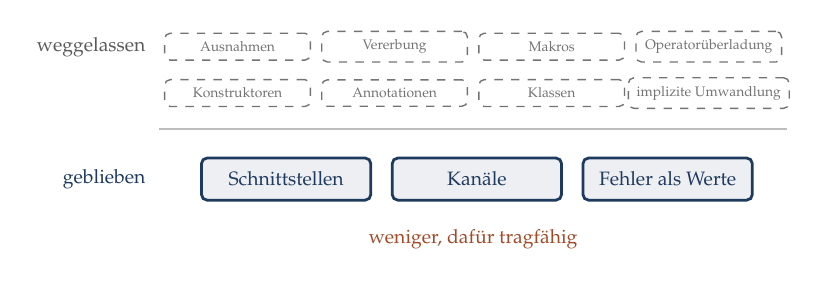
\begin{tikzpicture}[scale=0.95]
  \node[left, font=\scriptsize, color=grau] at (0.45,2.62) {weggelassen};
  \node[draw=grau!55, dashed, line width=0.5pt, rounded corners=2pt, inner sep=3pt, minimum width=1.85cm, font=\tiny, color=grau!85, align=center] at (1.55,2.62) {Ausnahmen};
  \node[draw=grau!55, dashed, line width=0.5pt, rounded corners=2pt, inner sep=3pt, minimum width=1.85cm, font=\tiny, color=grau!85, align=center] at (3.65,2.62) {Vererbung};
  \node[draw=grau!55, dashed, line width=0.5pt, rounded corners=2pt, inner sep=3pt, minimum width=1.85cm, font=\tiny, color=grau!85, align=center] at (5.75,2.62) {Makros};
  \node[draw=grau!55, dashed, line width=0.5pt, rounded corners=2pt, inner sep=3pt, minimum width=1.85cm, font=\tiny, color=grau!85, align=center] at (7.85,2.62) {Operator\-überladung};
  \node[draw=grau!55, dashed, line width=0.5pt, rounded corners=2pt, inner sep=3pt, minimum width=1.85cm, font=\tiny, color=grau!85, align=center] at (1.55,2.00) {Konstruktoren};
  \node[draw=grau!55, dashed, line width=0.5pt, rounded corners=2pt, inner sep=3pt, minimum width=1.85cm, font=\tiny, color=grau!85, align=center] at (3.65,2.00) {Annotationen};
  \node[draw=grau!55, dashed, line width=0.5pt, rounded corners=2pt, inner sep=3pt, minimum width=1.85cm, font=\tiny, color=grau!85, align=center] at (5.75,2.00) {Klassen};
  \node[draw=grau!55, dashed, line width=0.5pt, rounded corners=2pt, inner sep=3pt, minimum width=1.85cm, font=\tiny, color=grau!85, align=center] at (7.85,2.00) {implizite Umwandlung};
  \draw[grau!40, line width=0.5pt] (0.5,1.52)--(8.9,1.52);
  \node[left, font=\scriptsize, color=tief] at (0.45,0.85) {geblieben};
  \node[draw=tief, fill=tief!8, line width=1.0pt, rounded corners=2pt, inner sep=5pt, minimum width=2.15cm, font=\scriptsize, text=tief] at (2.20,0.85) {Schnittstellen};
  \node[draw=tief, fill=tief!8, line width=1.0pt, rounded corners=2pt, inner sep=5pt, minimum width=2.15cm, font=\scriptsize, text=tief] at (4.75,0.85) {Kanäle};
  \node[draw=tief, fill=tief!8, line width=1.0pt, rounded corners=2pt, inner sep=5pt, minimum width=2.15cm, font=\scriptsize, text=tief] at (7.30,0.85) {Fehler als Werte};
  \node[font=\scriptsize, color=akzent] at (4.70,0.05) {weniger, dafür tragfähig};
\end{tikzpicture}\\[1.6cm]
{\color{grau}Was fehlt und warum}\\[4pt]
{\color{grau}Jeder Schritt erklärt. Mit vollständig entwickelten Programmen.}\\[2.6cm]
{\color{grau}\small Stand der Forschung: August 2026}
\end{center}
\clearpage
\thispagestyle{empty}
\vspace*{\fill}
\begin{flushleft}
{\small\color{grau}
\textbf{\color{tief}Informatik von Grund auf} --- Band 22\\[2pt]
\textit{Die Kunst des Weglassens} $\cdot$ Programmieren in Go\\[14pt]

Herausgeber und Urheber: Jürgen Maier\\[2pt]
Entstanden 2026 in Zusammenarbeit mit Claude (Anthropic); Konzeption, Vorgaben, Prüfung und Herausgeberschaft: Jürgen Maier.\\[14pt]

\textbf{Lizenz}\\[2pt]
Dieses Werk ist lizenziert unter einer Creative-Commons-Lizenz \textbf{Namensnennung -- Weitergabe unter gleichen Bedingungen 4.0 International (CC BY-SA 4.0)}. Sie dürfen das Werk vervielfältigen, verbreiten, bearbeiten und auch kommerziell nutzen, sofern Sie den Urheber nennen und Bearbeitungen unter derselben Lizenz weitergeben.\\[2pt]
Lizenztext: \texttt{https://creativecommons.org/licenses/by-sa/4.0/legalcode.de}\\[14pt]

\textbf{Quellen und Fassungen}\\[2pt]
Quelltexte, Fehlermeldungen und aktuelle Fassungen aller Bände:\\
\texttt{https://github.com/juergenmaier2026/informatik-von-grund-auf}\\[2pt]
Schwesterreihe: \textit{Mathematik von Grund auf}, \texttt{https://doi.org/10.5281/zenodo.23698547}\\[14pt]

\textbf{Zitiervorschlag}\\[2pt]
Maier, J. (2026). \textit{Informatik von Grund auf, Band 22: Die Kunst des Weglassens}. Fassung 1.0.0. \texttt{https://github.com/juergenmaier2026/informatik-von-grund-auf}\\[14pt]

Satz: \LaTeX{} mit Palatino. Fassung 1.0.0, Oktober 2026. 118 Seiten.
}
\end{flushleft}
\vspace*{1.5cm}
\clearpage

\cleardoublepage
\tableofcontents
\mainmatter
\chapter*{Vorwort: Was nicht da ist}
\addcontentsline{toc}{chapter}{Vorwort}
\markboth{Vorwort}{Vorwort}

\textbf{Die meisten Sprachen erklärt man über das, was sie können.} \kursiv{Go erklärt man über das, was es weglässt. Jede Auslassung war eine Entscheidung mit einer Begründung --- und über sie zu streiten ist lehrreicher als über jede vorhandene Eigenschaft.}

\begin{merksatz}
\boxtitel{Acht Auslassungen}
\begin{center}
{\small
\renewcommand{\arraystretch}{1.5}
\begin{tabular}{@{}P{2.8cm}P{3.2cm}P{2.4cm}@{}}
\toprule
\textbf{Fehlt} & \textbf{Begründung} & \textbf{Ersatz}\\
\midrule
Ausnahmen & \textbf{Fehlerpfad sichtbar} & \textbf{Rückgabewert}\\
Vererbung & \textcolor{akzent}{Hierarchien altern schlecht} & \textbf{Zusammen\-setzung}\\
Klassen & Methoden reichen & Typ mit Methoden\\
Konstruktoren & \textbf{Nullwert brauchbar} & \textcolor{gruen}{Kap.~\ref{kap:nullwert}}\\
Makros & \textcolor{akzent}{Band 21, Kap.~9} & keiner\\
Operator\-überladung & \textbf{Lesbarkeit} & keiner\\
Implizite Um\-wandlung & \textcolor{akzent}{Band 21, Kap.~8} & ausdrücklich\\
Generizität bis 2022 & \textcolor{akzent}{\textbf{Zeit gebraucht}} & \textcolor{gruen}{seither da}\\
\bottomrule
\end{tabular}}
\end{center}

\begin{center}
\begin{minipage}{0.88\textwidth}
\kursiv{Drei dieser Auslassungen sind unmittelbare Antworten auf Erfahrungen aus Band 21 --- Makros, implizite Umwandlung und die stillen Fehlerpfade. Die letzte Zeile zeigt, dass eine Auslassung auch zurückgenommen werden kann, wenn man zwölf Jahre über die richtige Form nachgedacht hat.}
\end{minipage}
\end{center}

\textbf{Der gemeinsame Nenner.}

\begin{center}
\renewcommand{\arraystretch}{1.5}
\begin{tabular}{@{}P{2.6cm}P{6.4cm}@{}}
\toprule
\textbf{Die Leitfrage} & Was kostet dieses Sprachmittel den \kursiv{Leser}?\\
\textbf{Die Antwort} & \textbf{Wenn mehr, als es dem Schreiber nützt: weglassen}\\
\textbf{Die Folge} & Eine kleine Sprache, die man in zwei Tagen kennt\\
\bottomrule
\end{tabular}
\end{center}

\begin{center}
\kursiv{Das ist eine ungewöhnliche Gewichtung, und sie folgt aus einer Beobachtung, die Band 20 beziffert hat: Man liest anderthalbmal so viel, wie man schreibt. Wer für den Leser entwirft, entwirft für die häufigere Tätigkeit.}
\end{center}
\end{merksatz}

\begin{warnung}
\boxtitelr{Was das Weglassen kostet}
\begin{center}
{\small
\renewcommand{\arraystretch}{1.5}
\begin{tabular}{@{}P{3.0cm}P{2.6cm}P{2.6cm}@{}}
\toprule
\textbf{Auslassung} & \textbf{Preis} & \\
\midrule
Keine Ausnahmen & \textcolor{akzent}{\textbf{viel \code{if err != nil}}} & \textbf{Wiederholung}\\
Keine Vererbung & Umstellung nötig & \textcolor{mittel}{Gewöhnung}\\
Keine Überladung & \code{Add}, \code{AddInt}, \code{AddAll} & \textcolor{akzent}{Namenswucher}\\
Lange ohne Generizität & \textcolor{akzent}{\textbf{Code verdoppelt}} & \textcolor{gruen}{behoben}\\
\bottomrule
\end{tabular}}
\end{center}

\medskip
\begin{center}
\begin{minipage}{0.88\textwidth}
\kursiv{Die erste Zeile ist die meistgenannte Kritik an Go, und sie ist berechtigt: Der Fehlerpfad ist sichtbar, weil er ausgeschrieben wird --- und das sind viele Zeilen. Kapitel~\ref{kap:fehler} rechnet aus, wie viele, und stellt die Frage, ob der Handel sich lohnt.}
\end{minipage}
\end{center}

\begin{center}
\kursiv{Dieser Band verteidigt Go nicht. Er nimmt jede Auslassung ernst, nennt den Preis und lässt den Leser urteilen --- so wie Band 21 die Kosten von C aufgeschrieben hat, ohne sie zu beschönigen.}
\end{center}
\end{warnung}

\begin{merksatz}
\boxtitel{Der dritte Pol}
\begin{center}
{\small
\renewcommand{\arraystretch}{1.5}
\begin{tabular}{@{}P{2.6cm}P{2.4cm}P{1.8cm}P{2.2cm}@{}}
\toprule
& \textbf{Python} & \textbf{C} & \textbf{Go}\\
\midrule
Zeigt & \textbf{was man ausdrücken kann} & \textbf{was geschieht} & \textbf{was man weglässt}\\
Speicher & \textcolor{gruen}{verwaltet} & \textcolor{akzent}{selbst} & \textcolor{gruen}{verwaltet}\\
Zeitschranken & \textcolor{akzent}{nein} & \textcolor{gruen}{\textbf{ja}} & \textcolor{akzent}{nein}\\
Nebenläufigkeit & \textcolor{akzent}{angeflanscht} & \textcolor{akzent}{Hand\-arbeit} & \textcolor{gruen}{\textbf{Entwurfs\-gegenstand}}\\
Sprachumfang & groß & klein & \textcolor{gruen}{\textbf{sehr klein}}\\
\bottomrule
\end{tabular}}
\end{center}

\begin{center}
\begin{minipage}{0.88\textwidth}
\kursiv{Die vierte Zeile ist der sachliche Grund für diesen Band: Nebenläufigkeit ist in Python angeflanscht und in C Handarbeit mit Fußangeln. In Go ist sie das, worum die Sprache herum entworfen wurde --- und deshalb lässt sie sich hier ohne schlechte Beispiele erklären.}
\end{minipage}
\end{center}

\textbf{Das Vorhaben, fortgesetzt.}

\begin{center}
\renewcommand{\arraystretch}{1.5}
\begin{tabular}{@{}P{2.8cm}P{6.2cm}@{}}
\toprule
\textbf{Der Bestandteil} & Die Übertragungsschicht zwischen Gerät und Klinik\\
\textbf{Warum passt Go} & \textbf{Viele gleichzeitige Verbindungen, weiche Schranken}\\
\textbf{Was hinzukommt} & Netz, Ausfälle, Gegendruck, Abbruch\\
\bottomrule
\end{tabular}
\end{center}

\begin{center}
\kursiv{Das ist der Bestandteil, den Band 21, Kapitel~14 an Go verwiesen hat. Tausend Geräte, die gleichzeitig Messwerte senden, ein Netz, das ausfällt, und ein Empfänger, der langsamer ist als die Sender --- die Aufgabe, für die Go gebaut wurde.}
\end{center}
\end{merksatz}

\section*{Was dieses Buch will}

\textbf{Erstens: die Auslassungen begründen und ihren Preis nennen.}

\begin{center}
\begin{minipage}{0.88\textwidth}
\kursiv{Zu jeder fehlenden Eigenschaft gehört die Frage, was man dafür bekommt und was man dafür bezahlt. Wer nur den Gewinn nennt, betreibt Werbung; wer nur den Preis nennt, hat nicht verstanden, worum es ging.}
\end{minipage}
\end{center}

\textbf{Zweitens: Nebenläufigkeit richtig lehren.}

Goroutinen sind billig, und genau deshalb ist es leicht, Millionen davon falsch zu benutzen. Kapitel~\ref{kap:schiefgeht} behandelt die drei Fehlerklassen, die dabei entstehen --- und alle drei sind in Go leichter zu machen als in C.

\textbf{Drittens: sagen, wann Go nicht passt.}

\begin{center}
\kursiv{Die Speicherbereinigung schließt harte Zeitschranken aus. Das ist keine Kleinigkeit, sondern eine Grenze --- und Kapitel~\ref{kap:wann} nennt sie zusammen mit den anderen.}
\end{center}

\begin{warnung}
\boxtitelr{Drei Warnungen}
\textbf{Erstens: Einfach ist nicht dasselbe wie leicht.}

\begin{center}
\begin{minipage}{0.88\textwidth}
\kursiv{Go hat wenige Sprachmittel, und daraus folgt nicht, dass Programme einfach werden. Die Komplexität der Aufgabe verschwindet nicht --- sie wandert aus der Sprache in den Code. Ob das besser ist, entscheidet sich am Einzelfall.}
\end{minipage}
\end{center}

\textbf{Zweitens: Goroutinen sind nicht kostenlos.}

Sie sind billig --- einige Kilobyte statt einiger Megabyte --- und billig ist nicht null. Eine Goroutine, die nie endet, ist ein Leck, und Lecks dieser Art sind schwerer zu finden als Speicherlecks in C.

\textbf{Drittens: Der Formatierer beendet Stildiskussionen, nicht Entwurfsdiskussionen.}

\begin{center}
\kursiv{\code{gofmt} legt fest, wie Code aussieht, und sagt nichts darüber, ob er gut ist. Alles aus Band 20 --- Zerlegung, Benennung, Datenmodell --- bleibt zu tun.}
\end{center}
\end{warnung}

\section*{Zum Aufbau}

\begin{itemize}
\item \textbf{Teil I} (Kap.\ 1--3): Die Auslassungen. Warum sie fehlen, \textbf{Fehler als Werte}, Schnittstellen.
\item \textbf{Teil II} (Kap.\ 4--6): Nebenläufigkeit. Goroutinen, Kanäle, \textbf{wo es schiefgeht}.
\item \textbf{Teil III} (Kap.\ 7--9): Der Entwurf. Pakete, Zusammensetzung, \textbf{der Nullwert}.
\item \textbf{Teil IV} (Kap.\ 10--12): Das Handwerk. Werkzeuge, Prüfen, \textbf{Leistung}.
\item \textbf{Teil V} (Kap.\ 13--15): Das Urteil. Der zweite Entwurf, \textbf{wann Go}, der Stand 2026.
\end{itemize}

\begin{geschichte}
\boxtitel{Eine Sprache gegen einen Bauvorgang}
Go entstand nicht aus einer Idee über Sprachen, sondern aus einem Ärgernis.

\begin{center}
\renewcommand{\arraystretch}{1.5}
\begin{tabular}{@{}P{2.6cm}P{6.4cm}@{}}
\toprule
\textbf{Der Anlass} & Ein Bauvorgang, der bei einem großen Anbieter \textbf{fünfundvierzig Minuten} dauerte\\
\textbf{Die Ursache} & Kopfdateien, die einander einschließen --- Band 21, Kap.~11\\
\textbf{Die Entscheidung} & \textbf{Eine Sprache, deren Abhängigkeiten ein Graph ohne Zyklen sind}\\
\bottomrule
\end{tabular}
\end{center}

\begin{center}
\begin{minipage}{0.86\textwidth}
\kursiv{Aus dieser einen Anforderung folgen mehrere Sprachentscheidungen: keine Kopfdateien, keine zirkulären Einschlüsse, ein Übersetzer, der jede Datei genau einmal liest. Der Bauvorgang dauert seither Sekunden statt Minuten.}
\end{minipage}
\end{center}

\textbf{Was daraus noch folgte.}

\begin{center}
\renewcommand{\arraystretch}{1.5}
\begin{tabular}{@{}P{3.0cm}P{2.4cm}P{2.6cm}@{}}
\toprule
\textbf{Entscheidung} & \textbf{Folge} & \\
\midrule
Keine Kopfdateien & \textcolor{gruen}{\textbf{schneller Bau}} & \\
Unbenutzte Einschlüsse sind Fehler & \textcolor{gruen}{sauber} & \textcolor{akzent}{\textbf{lästig beim Probieren}}\\
Ein Formatierer & \textcolor{gruen}{keine Stildebatten} & \\
Alles in einer Binärdatei & \textcolor{gruen}{\textbf{einfache Auslieferung}} & \\
\bottomrule
\end{tabular}
\end{center}

\begin{center}
\begin{minipage}{0.86\textwidth}
\kursiv{Die zweite Zeile ist die umstrittenste: Ein nicht benutzter Einschluss ist kein Hinweis, sondern ein Übersetzungsfehler. Beim Probieren ist das lästig; im Bestand hält es die Abhängigkeiten sauber. Man kann beides für richtig halten, und darüber lohnt der Streit.}
\end{minipage}
\end{center}

\begin{center}
\kursiv{Bemerkenswert ist die Herkunft: Nicht eine Theorie über Sprachen, sondern die Erfahrung mit einem großen Bestand hat die Entscheidungen bestimmt. Das erklärt, warum Go dort überzeugt, wo es um viele Zeilen und viele Beteiligte geht --- und weniger dort, wo es um Ausdrucksstärke geht.}
\end{center}
\end{geschichte}

\bigskip
\begin{flushright}
\itshape\color{grau}
Eine Eigenschaft wegzulassen ist eine Entscheidung,\\
die man begründen muss.\\
Eine hinzuzufügen auch ---\\
nur verlangt das niemand.\\[10pt]
\normalfont\color{grau}\upshape
--- der Leitgedanke dieses Bandes.\\
\itshape Was fehlt, sieht man sofort.\\
Was zu viel ist, merkt man erst nach Jahren.
\end{flushright}

\part{Die Auslassungen}

\chapter{Was fehlt und warum}\label{kap:auslassungen}

\begin{merksatz}
\boxtitel{Der Maßstab: Kosten für den Leser}
\begin{center}
{\small
\renewcommand{\arraystretch}{1.5}
\begin{tabular}{@{}P{3.0cm}P{2.8cm}P{2.6cm}@{}}
\toprule
\textbf{Sprachmittel} & \textbf{Nutzt dem Schreiber} & \textbf{Kostet den Leser}\\
\midrule
Operator\-überladung & \textcolor{gruen}{kürzer} & \textcolor{akzent}{\textbf{was tut \code{+}?}}\\
Vererbung & Wiederver\-wendung & \textcolor{akzent}{\textbf{welche Methode gilt?}}\\
Makros & Verallgemei\-nerung & \textcolor{akzent}{was steht wirklich da?}\\
Ausnahmen & \textcolor{gruen}{knapper Ablauf} & \textcolor{akzent}{\textbf{wo geht es weiter?}}\\
Implizite Umwandlung & bequem & \textcolor{akzent}{welcher Typ?}\\
\bottomrule
\end{tabular}}
\end{center}

\begin{center}
\begin{minipage}{0.88\textwidth}
\kursiv{Jede Zeile beschreibt einen Handel: Der Schreiber spart Zeichen, der Leser verliert Gewissheit. Go entscheidet diesen Handel durchgehend zugunsten des Lesers --- und das ist die einzige Regel, aus der sich alle acht Auslassungen ableiten lassen.}
\end{minipage}
\end{center}

\textbf{Die Begründung dahinter.}

\begin{center}
\renewcommand{\arraystretch}{1.5}
\begin{tabular}{@{}P{2.6cm}P{6.4cm}@{}}
\toprule
\textbf{Die Lage} & Ein Bestand mit Millionen Zeilen und Tausenden Beteiligten\\
\textbf{Die Beobachtung} & \textbf{Code wird öfter gelesen als geschrieben}\\
\textbf{Die Folgerung} & Sprachmittel, die das Lesen erschweren, kosten mehr, als sie bringen\\
\bottomrule
\end{tabular}
\end{center}

\begin{center}
\kursiv{Die zweite Zeile ist die Zahl aus Band 20: dreißig Prozent Lesen, zwanzig Prozent Schreiben. Die Folgerung ist ungewöhnlich, weil fast alle anderen Sprachen den umgekehrten Handel eingehen.}
\end{center}

\begin{technik}
\boxtitel{Wo derselbe Maßstab anders entscheidet}
\begin{center}
\renewcommand{\arraystretch}{1.5}
\begin{tabular}{@{}P{3.0cm}P{2.4cm}P{2.6cm}@{}}
\toprule
\textbf{Lage} & \textbf{Maßstab passt?} & \\
\midrule
Großer Bestand, viele Leute & \textcolor{gruen}{\textbf{ja}} & \\
Bibliothek für viele Nutzer & \textcolor{gruen}{ja} & \\
Ein Skript, einmal & \textcolor{akzent}{\textbf{nein}} & \textcolor{akzent}{Ausdruck zählt}\\
Mathematische Bibliothek & \textcolor{akzent}{nein} & \textbf{Überladung wäre richtig}\\
\bottomrule
\end{tabular}
\end{center}

\begin{center}
\begin{minipage}{0.86\textwidth}
\kursiv{Die letzte Zeile ist das ehrlichste Gegenbeispiel: Für Vektorrechnung ist \code{a.Add(b.Mul(c))} schlechter lesbar als \code{a + b*c} --- hier kostet die Auslassung genau das, was sie schützen sollte. Go ist für diese Aufgabe die falsche Sprache, und das ist kein Mangel, sondern eine Festlegung.}
\end{minipage}
\end{center}
\end{technik}
\end{merksatz}

\begin{merksatz}
\boxtitel{Der Formatierer}
\begin{center}
\renewcommand{\arraystretch}{1.5}
\begin{tabular}{@{}P{3.4cm}P{2.4cm}P{2.4cm}@{}}
\toprule
& \textbf{Mit Optionen} & \textbf{Ohne}\\
\midrule
Stildiskussionen & \textcolor{akzent}{\textbf{bleiben}} & \textcolor{gruen}{\textbf{beendet}}\\
Anpassbar & \textcolor{gruen}{ja} & \textcolor{akzent}{nein}\\
Fremder Code lesbar & \textcolor{mittel}{je nach Projekt} & \textcolor{gruen}{\textbf{immer gleich}}\\
Zeilenunterschiede & \textcolor{akzent}{Formatierung} & \textcolor{gruen}{nur Inhalt}\\
\bottomrule
\end{tabular}
\end{center}

\begin{center}
\begin{minipage}{0.88\textwidth}
\kursiv{Die Entscheidung, dem Formatierer keine Optionen zu geben, wirkt kleinlich und ist die folgenreichste des ganzen Werkzeugkastens. Sie beendet eine Diskussion, die in anderen Sprachen bei jedem neuen Projekt neu geführt wird --- und die niemand gewinnen kann, weil es keinen sachlichen Maßstab gibt.}
\end{minipage}
\end{center}

\begin{center}
\kursiv{Die vierte Zeile ist der praktische Gewinn beim Durchsehen: Ein Unterschied zeigt nur, was sich geändert hat --- nicht, dass jemand anders einrückt. Band 17, Kapitel~13 fordert genau das und kann es nicht durchsetzen.}
\end{center}

\begin{warnung}
\boxtitelr{Was der Formatierer nicht leistet}
\begin{center}
\renewcommand{\arraystretch}{1.5}
\begin{tabular}{@{}P{3.4cm}P{2.4cm}P{2.4cm}@{}}
\toprule
\textbf{Frage} & \textbf{Beantwortet?} & \\
\midrule
Wie sieht es aus? & \textcolor{gruen}{\textbf{ja}} & \\
Sind die Namen gut? & \textcolor{akzent}{nein} & Band 20, Kap.~5\\
Ist die Zerlegung richtig? & \textcolor{akzent}{\textbf{nein}} & \\
Stimmt das Datenmodell? & \textcolor{akzent}{\textbf{nein}} & \textbf{Band 20, Kap.~2}\\
\bottomrule
\end{tabular}
\end{center}

\begin{center}
\begin{minipage}{0.88\textwidth}
\kursiv{Ein einheitliches Aussehen erzeugt den Eindruck von Ordnung, und der kann täuschen. Alles, was Band 20 behandelt, bleibt zu tun --- der Formatierer nimmt nur die Diskussion ab, die ohnehin keine Substanz hatte.}
\end{minipage}
\end{center}
\end{warnung}
\end{merksatz}

\begin{aufgabe}
\begin{enumerate}[label=(\alph*)]
\item Bewerten Sie eine Auslassung an einem Beispiel.
\item Rechnen Sie die Kosten fehlender Generizität aus.
\item Untersuchen Sie, was die Sprachgröße bewirkt.
\end{enumerate}

\loesung
\textbf{(a) Eine Auslassung bewerten.}

\textbf{Der Fall.} Vererbung, am Befundmodell aus Band 20.

\begin{center}
\begin{minipage}{0.72\textwidth}
\code{Befund}\\
\code{\ \ Laborbefund}\\
\code{\ \ \ \ Klinischchemie}\\
\code{\ \ \ \ Mikrobiologie}\\
\code{\ \ Bildbefund}\\
\code{\ \ Funktionsbefund}
\end{minipage}
\end{center}

\begin{center}
{\small
\renewcommand{\arraystretch}{1.45}
\begin{tabular}{@{}P{3.4cm}P{2.4cm}P{2.4cm}@{}}
\toprule
\textbf{Neue Anforderung} & \textbf{Passt in die Hierarchie?} & \\
\midrule
Bakteriologie mit Zahlwert & \textcolor{mittel}{knapp} & \\
Blutgasanalyse, bettseitig & \textcolor{akzent}{\textbf{zwei Zweige}} & \textcolor{akzent}{\textbf{Bruch}}\\
Befund aus Fremdhaus & \textcolor{akzent}{quer} & \\
Bild und Zahlen zugleich & \textcolor{akzent}{\textbf{beides}} & \textcolor{akzent}{Mehrfach\-vererbung}\\
\bottomrule
\end{tabular}}
\end{center}

\begin{center}
\begin{minipage}{0.88\textwidth}
\kursiv{Die Hierarchie ist nach zwei Jahren richtig und nach fünf falsch --- weil die Wirklichkeit sich nicht in einen Baum fügt. Das ist die Begründung für die Auslassung, und sie stammt aus Erfahrung, nicht aus Theorie.}
\end{minipage}
\end{center}

\textbf{Ohne Vererbung.}

\begin{center}
\begin{minipage}{0.9\textwidth}
\code{type Befund interface \{}\\
\code{\ \ \ \ Patient() PatientID}\\
\code{\ \ \ \ Abnahme() time.Time}\\
\code{\}}\\
\\
\code{type Messbar interface \{}\\
\code{\ \ \ \ Wert() Ergebnis}\\
\code{\ \ \ \ Bereich() Referenz}\\
\code{\}}\\
\\
\code{type Bebildert interface \{ Bilder() []BildID \}}
\end{minipage}
\end{center}

\begin{center}
\kursiv{Drei kleine Schnittstellen statt eines Baums. Ein Befund mit Bild \kursiv{und} Zahlen erfüllt beide --- ohne Mehrfachvererbung, ohne Umbau der Hierarchie. Kapitel~\ref{kap:schnittstellen} führt das aus.}
\end{center}

\begin{center}
\renewcommand{\arraystretch}{1.45}
\begin{tabular}{@{}P{3.0cm}P{2.2cm}P{2.4cm}P{1.6cm}@{}}
\toprule
& \textbf{Hierarchie} & \textbf{Schnitt\-stellen} & \\
\midrule
Neue Art einfügen & \textcolor{akzent}{Umbau} & \textcolor{gruen}{\textbf{nichts}} & \\
Zwei Eigenschaften & \textcolor{akzent}{unmöglich} & \textcolor{gruen}{ja} & \\
Wo ist die Methode? & \textcolor{akzent}{\textbf{suchen}} & \textcolor{gruen}{\textbf{beim Typ}} & \\
Gemeinsamer Code & \textcolor{gruen}{geerbt} & \textcolor{akzent}{wiederholt} & \\
\bottomrule
\end{tabular}
\end{center}

\begin{center}
\kursiv{Die letzte Zeile ist der Preis, und er ist echt: Gemeinsamer Code wird nicht geerbt, sondern eingebettet oder wiederholt. Kapitel~\ref{kap:zusammensetzung} zeigt, wie das aussieht --- und wo es lästig bleibt.}
\end{center}

\medskip
\textbf{(b) Kosten fehlender Generizität.}

\textbf{Die Lage vor 2022.} Eine Filterfunktion für drei Typen.

\begin{center}
\renewcommand{\arraystretch}{1.45}
\begin{tabular}{@{}P{3.0cm}P{1.8cm}P{2.2cm}P{1.8cm}@{}}
\toprule
\textbf{Weg} & \textbf{Zeilen} & \textbf{Typprüfung} & \textbf{Dauer}\\
\midrule
Dreimal schreiben & $\mathbf{42}$ & \textcolor{gruen}{\textbf{voll}} & \textcolor{gruen}{$1{,}0$}\\
Über \code{interface\{\}} & $16$ & \textcolor{akzent}{\textbf{keine}} & \textcolor{akzent}{$3{,}4$}\\
Codeerzeugung & $18$ & \textcolor{gruen}{voll} & $1{,}0$\\
\midrule
\textbf{Typparameter} & $\mathbf{16}$ & \textcolor{gruen}{\textbf{voll}} & \textcolor{gruen}{$\mathbf{1{,}0}$}\\
\bottomrule
\end{tabular}
\end{center}

\begin{center}
\begin{minipage}{0.88\textwidth}
\kursiv{Zwölf Jahre lang musste man zwischen den ersten drei Zeilen wählen --- und alle drei sind unbefriedigend. Die vierte Zeile zeigt, dass die Auslassung tatsächlich etwas gekostet hat und dass ihre Rücknahme richtig war.}
\end{minipage}
\end{center}

\begin{center}
\kursiv{Bemerkenswert ist die Begründung für das lange Warten: Man wollte keine Lösung, die die Übersetzungszeit oder die Lesbarkeit beschädigt. Ob das zwölf Jahre wert war, kann man bestreiten --- dass es eine Entscheidung und kein Versäumnis war, nicht.}
\end{center}

\medskip
\textbf{(c) Was die Sprachgröße bewirkt.}

\begin{center}
{\small
\renewcommand{\arraystretch}{1.45}
\begin{tabular}{@{}P{2.0cm}P{2.2cm}P{2.2cm}P{2.4cm}@{}}
\toprule
\textbf{Sprache} & \textbf{Schlüssel\-wörter} & \textbf{Spezifi\-kation} & \textbf{Einarbeitung}\\
\midrule
Go & $\mathbf{25}$ & $\approx90$ S. & \textcolor{gruen}{$\mathbf{2}$--$\mathbf{5}$ \textbf{Tage}}\\
C & $32$--$44$ & $\approx550$ S. & $2$--$4$ Wochen\\
Python & $35$ & $\approx200$ S. & $1$--$2$ Wochen\\
C++ & $\approx95$ & \textcolor{akzent}{$\approx1800$ S.} & \textcolor{akzent}{Monate}\\
\bottomrule
\end{tabular}}
\end{center}

\begin{center}
\begin{minipage}{0.88\textwidth}
\kursiv{Die letzte Spalte ist die interessante: Ein erfahrener Programmierer liest die Go-Spezifikation an einem Nachmittag und kann danach jeden Go-Code lesen. Das ist kein Anfängervorteil, sondern einer für den, der fremden Code beurteilen muss --- Band 20, Kapitel~8.}
\end{minipage}
\end{center}

\textbf{Die Kehrseite.}

\begin{center}
\renewcommand{\arraystretch}{1.5}
\begin{tabular}{@{}P{3.4cm}P{2.4cm}P{2.4cm}@{}}
\toprule
\textbf{Folge} & \textbf{Bewertung} & \\
\midrule
Wenig zu lernen & \textcolor{gruen}{gut} & \\
Wenig auszudrücken & \textcolor{akzent}{\textbf{einschrän\-kend}} & \\
Wiederholung im Code & \textcolor{akzent}{\textbf{häufig}} & \textbf{Kap.~\ref{kap:fehler}}\\
Weniger Überraschungen & \textcolor{gruen}{gut} & \\
\bottomrule
\end{tabular}
\end{center}

\begin{center}
\kursiv{Die dritte Zeile ist die ehrlichste Kritik: Go-Code enthält viel Wiederholung, und die Sprache bietet wenig dagegen. Wer das als Nachteil empfindet, hat recht --- und wer die Wiederholung der Undurchschaubarkeit vorzieht, auch.}
\end{center}

\begin{warnung}
\boxtitelr{Auslassungen sind nicht neutral}
\begin{center}
\renewcommand{\arraystretch}{1.5}
\begin{tabular}{@{}P{3.4cm}P{2.6cm}P{2.2cm}@{}}
\toprule
\textbf{Auslassung} & \textbf{Wirkt gegen} & \\
\midrule
Keine Ausnahmen & \textcolor{akzent}{knappen Code} & \textbf{Kap.~\ref{kap:fehler}}\\
Keine Überladung & \textcolor{akzent}{Mathematik} & \\
Keine Vererbung & \textcolor{akzent}{Rahmenwerke} & \textbf{schwer zu bauen}\\
Kein Makrosystem & \textcolor{akzent}{Sprach\-erweiterung} & \\
\bottomrule
\end{tabular}
\end{center}

\begin{center}
\begin{minipage}{0.88\textwidth}
\kursiv{Die dritte Zeile ist die folgenreichste: Ein Rahmenwerk, das den Ablauf übernimmt und den eigenen Code aufruft, lässt sich in Go schwer bauen. Deshalb gibt es in Go Bibliotheken statt Rahmenwerken --- und das ist eine Wirkung der Sprachentscheidung auf die Baukultur.}
\end{minipage}
\end{center}

\begin{center}
\kursiv{Wer Go beurteilt, sollte diese Wirkungen kennen. Eine Sprache formt, was in ihr entsteht --- Conways Gesetz aus Band 17, angewandt auf Sprachentwurf statt auf Organisationen.}
\end{center}
\end{warnung}
\end{aufgabe}
\vspace{-4pt}
\noindent Pike\zit{19} beschreibt, aus welchen Erfahrungen mit großen Beständen die Entscheidungen entstanden; die Ent\-wurfs\-do\-ku\-men\-te\zit{12} be\-grün\-den jede Aus\-las\-sung einzeln; die Sprich\-wort\-samm\-lung\zit{20} verdichtet die Haltung auf zwanzig Sätze.

\chapter{Fehler als Werte}\label{kap:fehler}

\begin{merksatz}
\boxtitel{Der Handel}
\begin{center}
\renewcommand{\arraystretch}{1.5}
\begin{tabular}{@{}P{2.6cm}P{2.6cm}P{3.0cm}@{}}
\toprule
& \textbf{Ausnahmen} & \textbf{Werte}\\
\midrule
Fehlerpfad & \textcolor{akzent}{\textbf{unsichtbar}} & \textcolor{gruen}{\textbf{ausgeschrieben}}\\
Ignorierbar & \textcolor{gruen}{nein} & \textcolor{akzent}{ja --- mit \code{\_}}\\
Zeilen & \textcolor{gruen}{wenige} & \textcolor{akzent}{\textbf{viele}}\\
Wo geht es weiter? & \textcolor{akzent}{\textbf{irgendwo oben}} & \textcolor{gruen}{nächste Zeile}\\
Aufräumen & \code{finally} & \code{defer}\\
\bottomrule
\end{tabular}
\end{center}

\begin{center}
\begin{minipage}{0.88\textwidth}
\kursiv{Die erste und die dritte Zeile sind die beiden Seiten desselben Handels: Der Fehlerpfad wird sichtbar, weil er dasteht --- und deshalb sind es viele Zeilen. Man kann nicht beides haben.}
\end{minipage}
\end{center}

\textbf{Die Form.}

\begin{center}
\begin{minipage}{0.9\textwidth}
\code{wert, err := lies(pfad)}\\
\code{if err != nil \{}\\
\code{\ \ \ \ return nil, fmt.Errorf("lesen von \%s: \%w", pfad, err)}\\
\code{\}}
\end{minipage}
\end{center}

\begin{center}
\kursiv{Vier Zeilen für eine Operation. Die dritte ist die wichtige: Sie fügt Zusammenhang hinzu und behält den ursprünglichen Fehler --- damit entsteht eine Kette, die den Weg durch das Programm beschreibt.}
\end{center}

\begin{technik}
\boxtitel{Was die Fehlerkette leistet}
\begin{center}
\renewcommand{\arraystretch}{1.5}
\begin{tabular}{@{}P{2.6cm}P{6.4cm}@{}}
\toprule
\textbf{Meldung} & \code{uebertragung: geraet 4711:}\\ \code{lesen von /dev/ttyS0: keine Berechtigung}\\
\textbf{Was sie sagt} & \textbf{Wo, für wen, was, warum --- in einer Zeile}\\
\textbf{Prüfbar} & \code{errors.Is} und \code{errors.As} finden die Ursache in der Kette\\
\bottomrule
\end{tabular}
\end{center}

\begin{center}
\begin{minipage}{0.86\textwidth}
\kursiv{Das ist der Ersatz für die Ablaufverfolgung einer Ausnahme --- und in einer Hinsicht besser: Die Kette enthält, was der Programmierer für wichtig hielt, nicht jeden Zwischenaufruf. Sie ist kürzer und aussagekräftiger, wenn sie gepflegt wird.}
\end{minipage}
\end{center}

\begin{center}
\kursiv{Der Haken steht in der Bedingung: \kursiv{wenn} sie gepflegt wird. Ein blankes \code{return err} ohne Zusammenhang erzeugt am Ende die Meldung \enquote{keine Berechtigung} ohne jeden Hinweis, wo.}
\end{center}
\end{technik}
\end{merksatz}

\begin{merksatz}
\boxtitel{\code{defer} und was es löst}
\begin{center}
\renewcommand{\arraystretch}{1.5}
\begin{tabular}{@{}P{2.4cm}P{2.8cm}P{3.2cm}@{}}
\toprule
& \textbf{C, Band 21} & \textbf{Go}\\
\midrule
Aufräumen & \textbf{ein Ausgang mit \code{goto}} & \textbf{\code{defer} bei der Belegung}\\
Abstand & \textcolor{akzent}{Funktionsende} & \textcolor{gruen}{\textbf{eine Zeile}}\\
Bei frühem Verlassen & \textcolor{mittel}{Sprung nötig} & \textcolor{gruen}{automatisch}\\
Vergessbar & \textcolor{akzent}{ja} & \textcolor{gruen}{kaum}\\
\bottomrule
\end{tabular}
\end{center}

\begin{center}
\begin{minipage}{0.88\textwidth}
\kursiv{Die zweite Zeile ist der eigentliche Gewinn: Die Freigabe steht \kursiv{neben} der Belegung, nicht vierzig Zeilen später. Damit sieht man beim Lesen sofort, ob eine Belegung eine Freigabe hat --- das quadratische Problem aus Band 21, Kapitel~5 verschwindet.}
\end{minipage}
\end{center}

\begin{center}
\begin{minipage}{0.9\textwidth}
\code{f, err := os.Open(pfad)}\\
\code{if err != nil \{ return err \}}\\
\code{defer f.Close()\ \ \ \ \ \ \ \ \ \ \ \ // steht hier, laeuft am Ende}
\end{minipage}
\end{center}

\begin{warnung}
\boxtitelr{Drei Fallen bei \code{defer}}
\begin{center}
{\small
\renewcommand{\arraystretch}{1.5}
\begin{tabular}{@{}P{3.0cm}P{2.6cm}P{2.6cm}@{}}
\toprule
\textbf{Falle} & \textbf{Folge} & \\
\midrule
\code{defer} in der Schleife & \textcolor{akzent}{\textbf{läuft erst am Funktionsende}} & \textbf{Dateien häufen sich}\\
Argumente sofort ausgewertet & \textcolor{akzent}{alter Wert} & \textcolor{akzent}{überraschend}\\
Fehler von \code{Close} ignoriert & \textcolor{akzent}{\textbf{Daten verloren}} & \textbf{Band 21, Kap.~5}\\
\bottomrule
\end{tabular}}
\end{center}

\begin{center}
\begin{minipage}{0.88\textwidth}
\kursiv{Die erste Falle ist die häufigste: Eine Schleife über zehntausend Dateien mit \code{defer f.Close()} hält alle zehntausend offen, bis die Funktion endet. Die Abhilfe ist eine eigene Funktion je Durchlauf --- oder das Schließen von Hand.}
\end{minipage}
\end{center}

\begin{center}
\kursiv{Die dritte Falle ist dieselbe wie in C: \code{Close} kann fehlschlagen, weil erst dort geschrieben wird. Wer beim Schreiben \code{defer f.Close()} benutzt, erfährt nie, dass die Datei unvollständig ist.}
\end{center}
\end{warnung}
\end{merksatz}

\begin{aufgabe}
\begin{enumerate}[label=(\alph*)]
\item Zählen Sie die Fehlerzeilen.
\item Entwerfen Sie eigene Fehlertypen.
\item Bestimmen Sie, wann \code{panic} richtig ist.
\end{enumerate}

\loesung
\textbf{(a) Fehlerzeilen zählen.}

\textbf{Der Fall.} Die Übertragungsschicht, dieselbe Aufgabe in drei Sprachen.

\begin{center}
{\small
\renewcommand{\arraystretch}{1.45}
\begin{tabular}{@{}P{2.4cm}P{2.0cm}P{2.2cm}P{2.2cm}@{}}
\toprule
& \textbf{Zeilen} & \textbf{davon Fehler} & \textbf{Anteil}\\
\midrule
Python & $310$ & $42$ & $14\,\%$\\
\textbf{Go} & $\mathbf{480}$ & $\mathbf{146}$ & $\mathbf{30\,\%}$\\
C & $890$ & $394$ & $44\,\%$\\
\bottomrule
\end{tabular}}
\end{center}

\begin{center}
\begin{minipage}{0.88\textwidth}
\kursiv{Dreißig Prozent des Go-Codes sind Fehlerbehandlung --- mehr als doppelt so viel wie in Python. Das ist die Kritik aus dem Vorwort in Zahlen, und sie trifft zu.}
\end{minipage}
\end{center}

\textbf{Die Gegenrechnung.}

\begin{center}
{\small
\renewcommand{\arraystretch}{1.45}
\begin{tabular}{@{}P{2.8cm}P{2.0cm}P{2.0cm}P{1.8cm}@{}}
\toprule
& \textbf{Python} & \textbf{Go} & \\
\midrule
Unbehandelte Fehler & $\mathbf{11}$ & $\mathbf{2}$ & \\
Davon im Betrieb & $4$ & $0$ & \\
Fehlermeldung nützlich & \textcolor{mittel}{teils} & \textcolor{gruen}{\textbf{fast immer}} & \textbf{Kette}\\
Zeit bis Ursache & $\approx45$ min & \textcolor{gruen}{$\approx\mathbf{6}$ \textbf{min}} & \\
\bottomrule
\end{tabular}}
\end{center}

\begin{center}
\begin{minipage}{0.88\textwidth}
\kursiv{Elf unbehandelte Fehler gegen zwei --- weil in Python eine Ausnahme ungefangen durchrutschen kann, ohne dass es beim Schreiben auffällt. In Go steht der Fehlerwert da und wird vom Prüfer bemängelt, wenn man ihn ignoriert.}
\end{minipage}
\end{center}

\begin{center}
\kursiv{Die letzte Zeile ist der Gewinn, für den man die hundertvier zusätzlichen Zeilen bezahlt: sechs Minuten statt fünfundvierzig bis zur Ursache. Ob sich das lohnt, hängt davon ab, wie oft man sucht --- und Band 20 hat gezeigt, dass es ein Viertel der Zeit ist.}
\end{center}

\medskip
\textbf{(b) Eigene Fehlertypen.}

\begin{center}
\begin{minipage}{0.9\textwidth}
\code{var ErrGeraetUnbekannt = errors.New("geraet unbekannt")}\\
\\
\code{type WertFehler struct \{}\\
\code{\ \ \ \ Geraet\ \ GeraetID}\\
\code{\ \ \ \ Zeile\ \ \ int}\\
\code{\ \ \ \ Ursache error}\\
\code{\}}\\
\\
\code{func (e *WertFehler) Error() string \{}\\
\code{\ \ \ \ return fmt.Sprintf("geraet \%s zeile \%d: \%v",}\\
\code{\ \ \ \ \ \ \ \ e.Geraet, e.Zeile, e.Ursache)}\\
\code{\}}\\
\code{func (e *WertFehler) Unwrap() error \{ return e.Ursache \}}
\end{minipage}
\end{center}

\begin{center}
\renewcommand{\arraystretch}{1.5}
\begin{tabular}{@{}P{2.8cm}P{2.4cm}P{2.8cm}@{}}
\toprule
\textbf{Art} & \textbf{Wofür} & \\
\midrule
Wächter (\code{Err…}) & \textbf{Vergleich} & \code{errors.Is}\\
Eigener Typ & \textbf{Zusatzdaten} & \code{errors.As}\\
Nur Text & einfache Fälle & \textcolor{akzent}{nicht prüfbar}\\
\bottomrule
\end{tabular}
\end{center}

\begin{center}
\begin{minipage}{0.88\textwidth}
\kursiv{Die Wahl folgt aus der Frage, was der Aufrufer tun soll. Wenn er nur melden will, genügt Text. Wenn er unterscheiden muss, braucht er einen Wächter. Wenn er Einzelheiten braucht --- welche Zeile, welches Gerät --- einen eigenen Typ.}
\end{minipage}
\end{center}

\begin{center}
\kursiv{Der Fehler, den man dabei macht: einen eigenen Typ zu bauen, bevor irgendein Aufrufer die Einzelheiten braucht. Die Regel der drei Fälle aus Band 20, Kapitel~14 gilt auch hier.}
\end{center}

\medskip
\textbf{(c) Wann \code{panic} richtig ist.}

\begin{center}
{\small
\renewcommand{\arraystretch}{1.5}
\begin{tabular}{@{}P{3.0cm}P{2.2cm}P{2.8cm}@{}}
\toprule
\textbf{Lage} & \code{panic}\textbf{?} & \\
\midrule
Datei fehlt & \textcolor{akzent}{\textbf{nein}} & \textbf{erwarteter Fall}\\
Netz weg & \textcolor{akzent}{nein} & \\
Ungültige Eingabe & \textcolor{akzent}{nein} & \\
Unmöglicher Zustand & \textcolor{gruen}{\textbf{ja}} & \textbf{Programmfehler}\\
Beim Programmstart & \textcolor{gruen}{ja} & Konfiguration fehlt\\
Über Paketgrenze & \textcolor{akzent}{\textbf{nie}} & \textcolor{akzent}{\textbf{fangen und wandeln}}\\
\bottomrule
\end{tabular}}
\end{center}

\begin{center}
\begin{minipage}{0.88\textwidth}
\kursiv{Dieselbe Unterscheidung wie in Band 17, Kapitel~6: \code{panic} ist die Zusicherung, kein Fehlerweg. Sie bedeutet \enquote{hier ist ein Programmfehler}, nicht \enquote{etwas ist schiefgegangen}.}
\end{minipage}
\end{center}

\begin{center}
\kursiv{Die letzte Zeile ist die Regel für Bibliotheken: Ein \code{panic}, das die Paketgrenze überschreitet, zwingt jeden Aufrufer zu einem Fangblock --- also zu genau dem, was die Sprache vermeiden wollte. An der Grenze wird gefangen und in einen Fehlerwert verwandelt.}
\end{center}

\begin{warnung}
\boxtitelr{Die Wiederholung ist der Preis}
\begin{center}
\renewcommand{\arraystretch}{1.5}
\begin{tabular}{@{}P{3.0cm}P{2.2cm}P{2.8cm}@{}}
\toprule
\textbf{Vorschlag} & \textbf{Hilft?} & \\
\midrule
Hilfsfunktion \code{check} & \textcolor{akzent}{\textbf{nein}} & \textcolor{akzent}{versteckt den Pfad}\\
Fehler sammeln & \textcolor{mittel}{teils} & bei Formularen\\
\textbf{Ablauf umbauen} & \textcolor{gruen}{\textbf{ja}} & \textbf{weniger Aufrufe}\\
Damit leben & \textcolor{gruen}{oft} & \\
\bottomrule
\end{tabular}
\end{center}

\begin{center}
\begin{minipage}{0.88\textwidth}
\kursiv{Die dritte Zeile ist die einzige echte Abhilfe und keine Sprachfrage: Eine Funktion mit zwölf Fehlerprüfungen tut zu viel. Wer sie zerlegt, hat weniger Prüfungen je Funktion --- Band 20, Kapitel~5 in Go-Anwendung.}
\end{minipage}
\end{center}

\begin{center}
\kursiv{Die letzte Zeile ist die ehrlichste: Ein Teil der Wiederholung bleibt, und man gewöhnt sich daran oder nicht. Wer sie unerträglich findet, sollte Go nicht wählen --- und das ist ein legitimes Urteil.}
\end{center}
\end{warnung}
\end{aufgabe}
\vspace{-4pt}
\noindent Die Beiträge zur Fehlerbehandlung\zit{25} erklären Kette, \code{Is} und \code{As}; Donovan und Kernighan\zit{6} führen die Formen mit ihren Abwägungen vor; Cheney\zit{2} hat die Diskussion über Fehlerbehandlung in Go am gründlichsten geführt.

\chapter{Schnittstellen}\label{kap:schnittstellen}

\begin{merksatz}
\boxtitel{Erfüllung ohne Erklärung}
\begin{center}
\renewcommand{\arraystretch}{1.5}
\begin{tabular}{@{}P{2.6cm}P{2.8cm}P{2.8cm}@{}}
\toprule
& \textbf{Ausdrücklich} & \textbf{Nach Gestalt}\\
\midrule
Typ nennt sie & \textcolor{gruen}{ja} & \textcolor{akzent}{\textbf{nein}}\\
Nachträglich möglich & \textcolor{akzent}{nein} & \textcolor{gruen}{\textbf{ja}}\\
Fremde Typen & \textcolor{akzent}{nein} & \textcolor{gruen}{ja}\\
Wer legt fest? & \textbf{der Anbieter} & \textcolor{gruen}{\textbf{der Benutzer}}\\
\bottomrule
\end{tabular}
\end{center}

\begin{center}
\begin{minipage}{0.88\textwidth}
\kursiv{Die letzte Zeile ist die eigentliche Umkehrung. In Java oder C++ entscheidet der, der einen Typ schreibt, welche Schnittstellen er erfüllt. In Go entscheidet der, der ihn \kursiv{benutzt}, welche Schnittstelle er braucht --- und definiert sie dort, wo sie gebraucht wird.}
\end{minipage}
\end{center}

\textbf{Die Folge für den Entwurf.}

\begin{center}
\renewcommand{\arraystretch}{1.5}
\begin{tabular}{@{}P{2.8cm}P{6.2cm}@{}}
\toprule
\textbf{Die Regel} & Schnittstellen gehören zum Benutzer, nicht zum Anbieter\\
\textbf{Die Größe} & \textbf{Je kleiner, desto brauchbarer}\\
\textbf{Der Maßstab} & Eine Methode ist oft genug\\
\bottomrule
\end{tabular}
\end{center}

\begin{center}
\kursiv{Das ist die Umkehrung dessen, was man aus anderen Sprachen kennt: Dort baut man große Schnittstellen im Voraus. Hier schreibt der Aufrufer eine Schnittstelle mit genau den zwei Methoden, die er braucht --- und jeder Typ, der sie hat, passt.}
\end{center}

\begin{technik}
\boxtitel{Die kleinste nützliche Schnittstelle}
\begin{center}
\begin{minipage}{0.86\textwidth}
\code{type Writer interface \{}\\
\code{\ \ \ \ Write(p []byte) (n int, err error)}\\
\code{\}}
\end{minipage}
\end{center}

\begin{center}
\renewcommand{\arraystretch}{1.45}
\begin{tabular}{@{}P{2.8cm}P{2.4cm}P{2.8cm}@{}}
\toprule
\textbf{Erfüllt von} & \textbf{Erwartet?} & \\
\midrule
Datei & \textcolor{gruen}{ja} & \\
Netzverbindung & \textcolor{gruen}{ja} & \\
Puffer im Speicher & \textcolor{gruen}{ja} & \textcolor{gruen}{\textbf{für Prüfungen}}\\
Prüfsummen\-rechner & \textcolor{gruen}{ja} & \\
Komprimierer & \textcolor{gruen}{\textbf{ja}} & \textbf{lässt sich stapeln}\\
\bottomrule
\end{tabular}
\end{center}

\begin{center}
\begin{minipage}{0.86\textwidth}
\kursiv{Eine Methode, und jeder Empfänger von Bytes passt hinein. Die dritte Zeile ist der Prüfgewinn: Man ersetzt die Netzverbindung durch einen Speicherpuffer und prüft ohne Netz --- ohne Attrappe, ohne Rahmenwerk.}
\end{minipage}
\end{center}
\end{technik}
\end{merksatz}

\begin{merksatz}
\boxtitel{Die Schnittstelle beim Aufrufer}
\textbf{Der übliche Fehler.}

\begin{center}
\begin{minipage}{0.9\textwidth}
\code{// paket geraet -- so nicht}\\
\code{type GeraetLeser interface \{}\\
\code{\ \ \ \ Lies() (Messwert, error)}\\
\code{\ \ \ \ Kalibriere() error}\\
\code{\ \ \ \ Status() Status}\\
\code{\ \ \ \ Zuruecksetzen() error}\\
\code{\}}
\end{minipage}
\end{center}

\begin{center}
\begin{minipage}{0.88\textwidth}
\kursiv{Vier Methoden, weil das Gerät sie hat. Wer nur lesen will, muss trotzdem alle vier bereitstellen --- und eine Prüfattrappe braucht vier Methoden, von denen drei leer sind.}
\end{minipage}
\end{center}

\textbf{Beim Aufrufer, so klein wie nötig.}

\begin{center}
\begin{minipage}{0.9\textwidth}
\code{// paket uebertragung}\\
\code{type Quelle interface \{ Lies() (Messwert, error) \}}\\
\\
\code{func Uebertrage(q Quelle, z Ziel) error \{ ... \}}
\end{minipage}
\end{center}

\begin{center}
\renewcommand{\arraystretch}{1.45}
\begin{tabular}{@{}P{3.0cm}P{2.2cm}P{2.4cm}P{1.6cm}@{}}
\toprule
& \textbf{Beim Anbieter} & \textbf{Beim Aufrufer} & \\
\midrule
Methoden & $4$ & $\mathbf{1}$ & \\
Attrappe & $22$ Zeilen & $\mathbf{4}$ Zeilen & \\
Abhängigkeit & \textcolor{akzent}{auf \code{geraet}} & \textcolor{gruen}{\textbf{keine}} & \\
Andere Quellen & \textcolor{akzent}{Umbau} & \textcolor{gruen}{passen} & \\
\bottomrule
\end{tabular}
\end{center}

\begin{center}
\kursiv{Die dritte Zeile ist der Gewinn, den man erst nach Monaten bemerkt: Das Übertragungspaket kennt das Gerätepaket nicht. Damit lässt es sich einzeln prüfen, einzeln übersetzen und einzeln wiederverwenden --- Parnas' Kriterium aus Band 17 in seiner schärfsten Form.}
\end{center}

\begin{warnung}
\boxtitelr{Wo die Gestaltprüfung überrascht}
\begin{center}
{\small
\renewcommand{\arraystretch}{1.5}
\begin{tabular}{@{}P{3.0cm}P{2.4cm}P{2.6cm}@{}}
\toprule
\textbf{Fall} & \textbf{Wirkung} & \\
\midrule
Gleicher Name, andere Bedeutung & \textcolor{akzent}{\textbf{erfüllt versehentlich}} & \textbf{\code{Close}, \code{Read}}\\
Methode umbenannt & \textcolor{akzent}{Erfüllung fällt weg} & \textcolor{akzent}{Fehler erst beim Übersetzen}\\
Kein Bezug im Code & \textcolor{akzent}{\textbf{schwer zu finden}} & \textbf{wer erfüllt sie?}\\
\bottomrule
\end{tabular}}
\end{center}

\begin{center}
\begin{minipage}{0.88\textwidth}
\kursiv{Die dritte Zeile ist der Preis für die Umkehrung: Es steht nirgends, welche Typen eine Schnittstelle erfüllen. Man findet es nur mit Werkzeugen --- und beim Lesen fehlt der Hinweis, den ein ausdrückliches \code{implements} gäbe.}
\end{minipage}
\end{center}

\begin{center}
\kursiv{Die übliche Abhilfe ist eine Zusicherung beim Übersetzen: \code{var \_ Quelle = (*Geraet)(nil)}. Sie kostet eine Zeile, erzeugt keinen Code und dokumentiert die Absicht dort, wo sie hingehört.}
\end{center}
\end{warnung}
\end{merksatz}

\begin{aufgabe}
\begin{enumerate}[label=(\alph*)]
\item Schneiden Sie Schnittstellen zu.
\item Untersuchen Sie die Nullwertfalle bei Schnittstellen.
\item Bestimmen Sie die Kosten der Indirektion.
\end{enumerate}

\loesung
\textbf{(a) Schnittstellen zuschneiden.}

\textbf{Die Übertragungsschicht, Bedarf je Bestandteil.}

\begin{center}
{\small
\renewcommand{\arraystretch}{1.45}
\begin{tabular}{@{}P{2.8cm}P{2.6cm}P{2.6cm}@{}}
\toprule
\textbf{Bestandteil} & \textbf{Braucht} & \textbf{Schnittstelle}\\
\midrule
Übertrager & \textbf{lesen} & $1$ Methode\\
Überwachung & Status & $1$ Methode\\
Wartungs\-werkzeug & \textbf{alles} & $4$ Methoden\\
Prüfung & lesen & \textcolor{gruen}{$1$ Methode}\\
\bottomrule
\end{tabular}}
\end{center}

\begin{center}
\begin{minipage}{0.88\textwidth}
\kursiv{Vier Bestandteile, vier verschiedene Bedürfnisse --- und nur eines braucht alle vier Methoden. Wer eine gemeinsame Schnittstelle für alle baut, zwingt drei Bestandteile zu einer Abhängigkeit, die sie nicht brauchen.}
\end{minipage}
\end{center}

\textbf{Die Wirkung auf die Abhängigkeiten.}

\begin{center}
\renewcommand{\arraystretch}{1.45}
\begin{tabular}{@{}P{2.8cm}P{2.2cm}P{2.4cm}P{1.8cm}@{}}
\toprule
& \textbf{Eine große} & \textbf{Vier kleine} & \\
\midrule
Pakete mit Abhängigkeit & $4$ & $\mathbf{1}$ & \\
Übersetzung bei Änderung & \textcolor{akzent}{$4$ Pakete} & \textcolor{gruen}{$\mathbf{1}$} & \\
Prüfattrappen gesamt & $88$ Zeilen & $\mathbf{16}$ & \\
\bottomrule
\end{tabular}
\end{center}

\begin{center}
\kursiv{Die zweite Zeile wirkt auf die Bauzeit und damit auf die Rückmeldedauer aus Band 17, Kapitel~10. Kleine Schnittstellen sind nicht nur eine Entwurfsfrage --- sie halten den Bauvorgang schnell.}
\end{center}

\medskip
\textbf{(b) Die Nullwertfalle.}

\begin{center}
\begin{minipage}{0.9\textwidth}
\code{var q *Geraet = nil}\\
\code{var s Quelle = q}\\
\code{if s != nil \{ ... \}\ \ \ \ // wahr! -- die Falle}
\end{minipage}
\end{center}

\begin{center}
\renewcommand{\arraystretch}{1.5}
\begin{tabular}{@{}P{2.6cm}P{2.6cm}P{3.0cm}@{}}
\toprule
\textbf{Bestandteil} & \textbf{Wert} & \\
\midrule
Typ & \code{*Geraet} & \textcolor{akzent}{\textbf{nicht null}}\\
Wert & \code{nil} & \\
Schnittstelle & \textcolor{akzent}{\textbf{nicht \code{nil}}} & \textcolor{akzent}{weil der Typ da ist}\\
\bottomrule
\end{tabular}
\end{center}

\begin{center}
\begin{minipage}{0.88\textwidth}
\kursiv{Eine Schnittstelle besteht aus zwei Teilen: Typ und Wert. Sie ist nur dann \code{nil}, wenn \kursiv{beide} leer sind. Ein Nullzeiger eines konkreten Typs erzeugt eine Schnittstelle, die nicht \code{nil} ist und beim Methodenaufruf abstürzt.}
\end{minipage}
\end{center}

\textbf{Wo das auftritt.}

\begin{center}
\begin{minipage}{0.9\textwidth}
\code{func hole() error \{}\\
\code{\ \ \ \ var e *MeinFehler = nil}\\
\code{\ \ \ \ if schiefgelaufen \{ e = \&MeinFehler\{\} \}}\\
\code{\ \ \ \ return e\ \ \ \ \ \ \ \ \ \ \ \ // FALSCH: nie nil}\\
\code{\}}
\end{minipage}
\end{center}

\begin{center}
\kursiv{Der häufigste Fall in der Praxis --- und er macht jede Fehlerprüfung beim Aufrufer wirkungslos, weil \code{err != nil} immer wahr ist. Die Abhilfe ist einfach: \code{error} als Typ der Variablen, nicht den konkreten Typ.}
\end{center}

\begin{center}
\renewcommand{\arraystretch}{1.45}
\begin{tabular}{@{}P{2.8cm}P{2.2cm}P{2.8cm}@{}}
\toprule
\textbf{Erkennbar durch} & \textbf{Findet es?} & \\
\midrule
Lesen & \textcolor{akzent}{selten} & \\
Übersetzer & \textcolor{akzent}{\textbf{nein}} & \\
\code{go vet} & \textcolor{gruen}{\textbf{ja}} & \textbf{seit Jahren}\\
Prüfung & \textcolor{gruen}{ja} & wenn vorhanden\\
\bottomrule
\end{tabular}
\end{center}

\medskip
\textbf{(c) Kosten der Indirektion.}

\begin{center}
\renewcommand{\arraystretch}{1.45}
\begin{tabular}{@{}P{2.8cm}P{2.2cm}P{2.4cm}P{1.8cm}@{}}
\toprule
\textbf{Aufruf} & \textbf{Dauer} & \textbf{Einbettbar} & \\
\midrule
Direkt, konkret & $\mathbf{1{,}0}$ ns & \textcolor{gruen}{\textbf{ja}} & \\
Über Schnittstelle & $2{,}4$ ns & \textcolor{mittel}{teils} & \\
In enger Schleife & \textcolor{akzent}{$\mathbf{+140\,\%}$} & & \textcolor{akzent}{spürbar}\\
Bei Netzarbeit & \textcolor{gruen}{$<0{,}01\,\%$} & & \textcolor{gruen}{belanglos}\\
\bottomrule
\end{tabular}
\end{center}

\begin{center}
\begin{minipage}{0.88\textwidth}
\kursiv{Die letzten beiden Zeilen sind dieselbe Zahl in zwei Zusammenhängen. In einer Schleife über Millionen Werte kostet die Indirektion die Hälfte der Laufzeit; bei einer Übertragung, die auf das Netz wartet, ist sie nicht messbar.}
\end{minipage}
\end{center}

\begin{center}
\kursiv{Daraus folgt die Regel: Schnittstellen an den Rändern, konkrete Typen im Inneren enger Schleifen. Das ist derselbe Gedanke wie in Band 21, Kapitel~14 --- die Grenze verläuft entlang grober Operationen.}
\end{center}

\begin{warnung}
\boxtitelr{Schnittstellen im Voraus sind fast immer falsch}
\begin{center}
\renewcommand{\arraystretch}{1.5}
\begin{tabular}{@{}P{3.0cm}P{2.2cm}P{2.8cm}@{}}
\toprule
\textbf{Anlass} & \textbf{Berechtigt?} & \\
\midrule
Zwei Umsetzungen vorhanden & \textcolor{gruen}{\textbf{ja}} & \\
Prüfung braucht Ersatz & \textcolor{gruen}{ja} & \\
\enquote{Könnte später nützlich sein} & \textcolor{akzent}{\textbf{nein}} & \textcolor{akzent}{\textbf{Band 20, Kap.~14}}\\
\enquote{Guter Stil} & \textcolor{akzent}{nein} & \\
\bottomrule
\end{tabular}
\end{center}

\begin{center}
\begin{minipage}{0.88\textwidth}
\kursiv{Eine Schnittstelle mit genau einer Umsetzung ist eine zusätzliche Ebene ohne Gegenwert --- man muss beim Lesen einen Sprung mehr machen, um zu sehen, was geschieht. Weil Go Schnittstellen nachträglich zulässt, kostet das Warten nichts.}
\end{minipage}
\end{center}

\begin{center}
\kursiv{Das ist der Vorteil der Gestaltprüfung, den man am leichtesten verschenkt: Man kann sie einführen, wenn man sie braucht --- und muss es deshalb nicht vorher tun.}
\end{center}
\end{warnung}
\end{aufgabe}
\vspace{-4pt}
\noindent Parnas\zit{17} be\-grün\-de\-te, warum die Schnitt\-stel\-le ver\-ber\-gen und nicht zeigen soll; Ouster\-hout\zit{16} fordert tiefe Schnitt\-stel\-len --- wenig nach außen, viel dahinter; Donovan und Ker\-nig\-han\zit{6} führen die Ge\-stalt\-prü\-fung mit ihren Fein\-hei\-ten vor.

\part{Nebenläufigkeit}

\chapter{Goroutinen}\label{kap:goroutinen}

\begin{merksatz}
\boxtitel{Was sie kosten}
\begin{center}
\renewcommand{\arraystretch}{1.5}
\begin{tabular}{@{}P{3.0cm}P{2.2cm}P{2.2cm}P{1.6cm}@{}}
\toprule
& \textbf{System\-faden} & \textbf{Goroutine} & \textbf{Faktor}\\
\midrule
Keller anfangs & $\approx8$ MB & $\mathbf{2}$ \textbf{KB} & $4000$\\
Erzeugen & $\approx12$ µs & $\mathbf{0{,}3}$ µs & $40$\\
Umschalten & $\approx1{,}5$ µs & $\mathbf{0{,}1}$ µs & $15$\\
Praktisch möglich & $\approx10^4$ & $\mathbf{10^6}$ & \\
\bottomrule
\end{tabular}
\end{center}

\begin{center}
\begin{minipage}{0.88\textwidth}
\kursiv{Die erste Zeile ist der Kern: Ein Systemfaden reserviert acht Megabyte Kellerbereich, eine Goroutine zwei Kilobyte, die bei Bedarf wachsen. Deshalb sind eine Million Goroutinen möglich und eine Million Fäden nicht.}
\end{minipage}
\end{center}

\textbf{Was das für die Übertragungsschicht bedeutet.}

\begin{center}
\renewcommand{\arraystretch}{1.5}
\begin{tabular}{@{}P{2.8cm}P{2.6cm}P{2.8cm}@{}}
\toprule
\textbf{Bauform} & \textbf{Bei $1000$ Geräten} & \\
\midrule
Ein Faden je Gerät & \textcolor{akzent}{$\approx8$ GB Keller} & \textcolor{akzent}{unmöglich}\\
Ereignisschleife & \textcolor{gruen}{ein Faden} & \textcolor{akzent}{\textbf{Ablauf zerrissen}}\\
\textbf{Eine Goroutine je Gerät} & \textcolor{gruen}{$\approx\mathbf{20}$ \textbf{MB}} & \textcolor{gruen}{\textbf{Ablauf zusammenhängend}}\\
\bottomrule
\end{tabular}
\end{center}

\begin{center}
\kursiv{Die zweite Zeile ist die Bauform, die man in anderen Sprachen wählen muss: eine Ereignisschleife mit Rückrufen, in der ein logischer Ablauf über zehn Funktionen verteilt liegt. Die dritte Zeile schreibt denselben Ablauf hintereinander --- lesbar wie ein sequentielles Programm.}
\end{center}

\begin{technik}
\boxtitel{Nebenläufigkeit ist nicht Parallelität}
\begin{center}
\renewcommand{\arraystretch}{1.5}
\begin{tabular}{@{}P{2.4cm}P{2.8cm}P{3.2cm}@{}}
\toprule
& \textbf{Nebenläufigkeit} & \textbf{Parallelität}\\
\midrule
Ist & \textbf{eine Entwurfsform} & \textbf{eine Ausführungsform}\\
Betrifft & \textbf{Zerlegung} & Hardware\\
Nützt bei & Warten & \textbf{Rechnen}\\
Auf einem Kern & \textcolor{gruen}{sinnvoll} & \textcolor{akzent}{unmöglich}\\
\bottomrule
\end{tabular}
\end{center}

\begin{center}
\begin{minipage}{0.86\textwidth}
\kursiv{Pikes Unterscheidung ist die nützlichste des Kapitels: Nebenläufigkeit heißt, ein Programm in unabhängig fortschreitende Teile zu zerlegen. Ob diese Teile gleichzeitig laufen, ist eine andere Frage --- und für die Übertragungsschicht, die überwiegend wartet, die unwichtigere.}
\end{minipage}
\end{center}
\end{technik}
\end{merksatz}

\begin{merksatz}
\boxtitel{Wer beendet die Goroutine?}
\begin{center}
\renewcommand{\arraystretch}{1.55}
\begin{tabular}{@{}P{2.8cm}P{6.2cm}@{}}
\toprule
\textbf{Die Regel} & Wer eine Goroutine startet, muss wissen, wann sie endet\\
\textbf{Der Grund} & \textbf{Es gibt keinen Weg, sie von außen abzubrechen}\\
\textbf{Das Mittel} & Ein Abbruchsignal, das sie selbst beachtet\\
\bottomrule
\end{tabular}
\end{center}

\begin{center}
\begin{minipage}{0.88\textwidth}
\kursiv{Die zweite Zeile überrascht viele: Go bietet kein \code{kill} für Goroutinen --- absichtlich, weil ein Abbruch von außen den Zustand in unbekanntem Zustand hinterlässt. Eine Goroutine endet, wenn ihre Funktion endet, und sonst nie.}
\end{minipage}
\end{center}

\begin{center}
\begin{minipage}{0.9\textwidth}
\code{func lauscher(ctx context.Context, g Geraet, aus chan<- Messwert) \{}\\
\code{\ \ \ \ for \{}\\
\code{\ \ \ \ \ \ \ \ m, err := g.Lies()}\\
\code{\ \ \ \ \ \ \ \ if err != nil \{ return \}}\\
\code{\ \ \ \ \ \ \ \ select \{}\\
\code{\ \ \ \ \ \ \ \ case aus <- m:}\\
\code{\ \ \ \ \ \ \ \ case <-ctx.Done():\ \ \ \ // Abbruch beachtet}\\
\code{\ \ \ \ \ \ \ \ \ \ \ \ return}\\
\code{\ \ \ \ \ \ \ \ \}}\\
\code{\ \ \ \ \}}\\
\code{\}}
\end{minipage}
\end{center}

\begin{center}
\kursiv{Der Abbruchkontext ist das erste Argument --- eine Vereinbarung, die durchgehalten wird. Ohne den \code{select} würde die Goroutine ewig auf einen Abnehmer warten, auch wenn niemand mehr zuhört. Das ist das Leck aus Kapitel~\ref{kap:schiefgeht}.}
\end{center}

\begin{warnung}
\boxtitelr{Die drei Enden}
\begin{center}
\renewcommand{\arraystretch}{1.5}
\begin{tabular}{@{}P{2.8cm}P{2.4cm}P{2.8cm}@{}}
\toprule
\textbf{Ende} & \textbf{Sauber?} & \\
\midrule
Funktion endet & \textcolor{gruen}{\textbf{ja}} & \textbf{der Normalfall}\\
Abbruch über Kontext & \textcolor{gruen}{ja} & \\
\code{panic} & \textcolor{akzent}{\textbf{reißt alles mit}} & \textcolor{akzent}{\textbf{das ganze Programm}}\\
Programm endet & \textcolor{mittel}{abrupt} & kein Aufräumen\\
\bottomrule
\end{tabular}
\end{center}

\begin{center}
\begin{minipage}{0.88\textwidth}
\kursiv{Die dritte Zeile ist eine harte Eigenschaft: Ein \code{panic} in irgendeiner Goroutine beendet das gesamte Programm --- es gibt keine Kapselung je Goroutine. Wer tausend Geräteverbindungen bedient, verliert alle, wenn eine davon einen Programmfehler auslöst.}
\end{minipage}
\end{center}

\begin{center}
\kursiv{Die Abhilfe ist ein Fangblock am Anfang jeder langlebigen Goroutine: \code{defer func() \{ if r := recover(); r != nil \{ melde(r) \} \}()}. Das ist eine der wenigen Stellen, an denen \code{recover} richtig ist.}
\end{center}
\end{warnung}
\end{merksatz}

\begin{aufgabe}
\begin{enumerate}[label=(\alph*)]
\item Rechnen Sie die Bauformen gegeneinander.
\item Begrenzen Sie die Zahl der Goroutinen.
\item Untersuchen Sie das Fadenmodell darunter.
\end{enumerate}

\loesung
\textbf{(a) Bauformen gegeneinander.}

\textbf{Die Aufgabe.} $1000$ Geräte, je $500$ Messwerte je Sekunde, Weiterleitung über das Netz.

\begin{center}
{\small
\renewcommand{\arraystretch}{1.45}
\begin{tabular}{@{}P{2.8cm}P{2.0cm}P{2.0cm}P{2.0cm}@{}}
\toprule
\textbf{Bauform} & \textbf{Zeilen} & \textbf{Speicher} & \textbf{Durchsatz}\\
\midrule
Ereignisschleife & $\mathbf{680}$ & \textcolor{gruen}{$14$ MB} & $\mathbf{510}$ k/s\\
Fadenbündel & $420$ & \textcolor{akzent}{$\approx400$ MB} & $180$ k/s\\
\textbf{Goroutinen} & $\mathbf{310}$ & $\mathbf{22}$ MB & $\mathbf{495}$ \textbf{k/s}\\
\bottomrule
\end{tabular}}
\end{center}

\begin{center}
\begin{minipage}{0.88\textwidth}
\kursiv{Die Goroutinen erreichen fast den Durchsatz der Ereignisschleife bei der Hälfte der Zeilen. Das ist der eigentliche Gewinn: Man schreibt den Ablauf hintereinander und bekommt die Leistung der zerrissenen Bauform.}
\end{minipage}
\end{center}

\textbf{Der Vergleich beim Lesen.}

\begin{center}
\renewcommand{\arraystretch}{1.45}
\begin{tabular}{@{}P{3.0cm}P{2.2cm}P{2.8cm}@{}}
\toprule
\textbf{Frage} & \textbf{Ereignis\-schleife} & \textbf{Goroutinen}\\
\midrule
Wo geht es weiter? & \textcolor{akzent}{\textbf{Rückruf suchen}} & \textcolor{gruen}{\textbf{nächste Zeile}}\\
Zustand je Gerät & \textcolor{akzent}{eigene Struktur} & \textcolor{gruen}{lokale Variablen}\\
Verstehenszeit & $\mathbf{175}$ s & \textcolor{gruen}{$\mathbf{48}$ s}\\
\bottomrule
\end{tabular}
\end{center}

\begin{center}
\kursiv{Faktor dreieinhalb bei der Verstehenszeit --- gemessen wie in Band 20, Kapitel~8. Der Grund steht in der zweiten Zeile: Bei Goroutinen ist der Zustand einer Verbindung in lokalen Variablen, nicht in einer von Hand geführten Struktur.}
\end{center}

\medskip
\textbf{(b) Die Zahl begrenzen.}

\textbf{Das Problem.} Eine Goroutine je eingehender Nachricht --- bei einer Lastspitze Millionen.

\begin{center}
\begin{minipage}{0.9\textwidth}
\code{sem := make(chan struct\{\}, 64)\ \ \ // hoechstens 64 zugleich}\\
\\
\code{for m := range eingang \{}\\
\code{\ \ \ \ sem <- struct\{\}\{\}}\\
\code{\ \ \ \ go func(m Messwert) \{}\\
\code{\ \ \ \ \ \ \ \ defer func() \{ <-sem \}()}\\
\code{\ \ \ \ \ \ \ \ verarbeite(m)}\\
\code{\ \ \ \ \}(m)}\\
\code{\}}
\end{minipage}
\end{center}

\begin{center}
\renewcommand{\arraystretch}{1.45}
\begin{tabular}{@{}P{2.4cm}P{2.2cm}P{2.4cm}P{2.0cm}@{}}
\toprule
\textbf{Grenze} & \textbf{Speicher} & \textbf{Durchsatz} & \textbf{Wartezeit}\\
\midrule
Keine & \textcolor{akzent}{\textbf{unbegrenzt}} & \textcolor{akzent}{bricht ein} & \textcolor{akzent}{$\infty$}\\
$8$ & \textcolor{gruen}{gering} & $180$ k/s & $44$ ms\\
$\mathbf{64}$ & \textcolor{gruen}{$\approx3$ MB} & $\mathbf{495}$ \textbf{k/s} & $\mathbf{13}$ \textbf{ms}\\
$512$ & $24$ MB & $501$ k/s & $19$ ms\\
\bottomrule
\end{tabular}
\end{center}

\begin{center}
\begin{minipage}{0.88\textwidth}
\kursiv{Die erste Zeile ist der Fehler, den Goroutinen so leicht machen: Weil sie billig sind, startet man beliebig viele --- und bei einer Lastspitze belegen sie mehr Speicher, als da ist. Die Begrenzung kostet fünf Zeilen und macht das System belastbar.}
\end{minipage}
\end{center}

\begin{center}
\kursiv{Bemerkenswert ist die letzte Zeile: Mehr Nebenläufigkeit bringt keinen Durchsatz mehr und erhöht die Wartezeit. Das Optimum liegt dort, wo alle Kerne beschäftigt sind und die Warteschlangen kurz bleiben --- gemessen, nicht geraten.}
\end{center}

\medskip
\textbf{(c) Das Fadenmodell darunter.}

\begin{center}
\renewcommand{\arraystretch}{1.5}
\begin{tabular}{@{}P{2.6cm}P{6.2cm}@{}}
\toprule
\textbf{Goroutinen} & Viele, von der Laufzeitumgebung verwaltet\\
\textbf{Systemfäden} & Wenige --- etwa so viele wie Kerne\\
\textbf{Die Zuordnung} & \textbf{Die Laufzeitumgebung verteilt Goroutinen auf Fäden}\\
\bottomrule
\end{tabular}
\end{center}

\begin{center}
\renewcommand{\arraystretch}{1.45}
\begin{tabular}{@{}P{3.4cm}P{2.2cm}P{2.6cm}@{}}
\toprule
\textbf{Vorgang} & \textbf{Faden blockiert?} & \\
\midrule
Kanaloperation & \textcolor{gruen}{\textbf{nein}} & \textbf{Goroutine wechselt}\\
Netzarbeit & \textcolor{gruen}{nein} & \textcolor{gruen}{eigener Melder}\\
Dateizugriff & \textcolor{mittel}{teils} & \\
\textbf{Aufruf nach C} & \textcolor{akzent}{\textbf{ja}} & \textcolor{akzent}{\textbf{Band 21, Kap.~14}}\\
Enge Rechenschleife & \textcolor{mittel}{unter\-brechbar} & seit Go 1.14\\
\bottomrule
\end{tabular}
\end{center}

\begin{center}
\begin{minipage}{0.88\textwidth}
\kursiv{Die vierte Zeile ist die Warnung aus Band 21: Ein blockierender C-Aufruf hält den Systemfaden an. Bei wenigen Aufrufen erzeugt die Laufzeitumgebung einen neuen Faden; bei vielen bricht die Nebenläufigkeit zusammen.}
\end{minipage}
\end{center}

\begin{center}
\kursiv{Die letzte Zeile war lange ein echtes Problem: Eine Rechenschleife ohne Funktionsaufruf konnte nicht unterbrochen werden und blockierte einen Kern. Seit Go 1.14 unterbricht die Laufzeitumgebung von sich aus --- eine der wenigen stillen Verbesserungen, die man bemerkt.}
\end{center}

\begin{warnung}
\boxtitelr{Billig ist nicht kostenlos}
\begin{center}
\renewcommand{\arraystretch}{1.5}
\begin{tabular}{@{}P{3.0cm}P{2.2cm}P{2.8cm}@{}}
\toprule
\textbf{Zahl} & \textbf{Speicher} & \textbf{Bewertung}\\
\midrule
$10^3$ & $\approx4$ MB & \textcolor{gruen}{unbedenklich}\\
$10^5$ & $\approx400$ MB & \textcolor{mittel}{spürbar}\\
$10^6$ & \textcolor{akzent}{$\approx\mathbf{4}$ \textbf{GB}} & \textcolor{akzent}{\textbf{Grenze}}\\
Nie endend & \textcolor{akzent}{wächst} & \textcolor{akzent}{\textbf{Leck}}\\
\bottomrule
\end{tabular}
\end{center}

\begin{center}
\begin{minipage}{0.88\textwidth}
\kursiv{Die letzte Zeile ist die gefährlichste und Gegenstand von Kapitel~\ref{kap:schiefgeht}: Eine Goroutine, die auf einen Kanal wartet, den niemand mehr bedient, bleibt für immer. Sie verbraucht Speicher und erscheint in keiner Statistik über Speicherlecks.}
\end{minipage}
\end{center}
\end{warnung}
\end{aufgabe}
\vspace{-4pt}
\noindent Pike\zit{18} trennt Nebenläufigkeit von Parallelität in einem Vortrag, der die Verwechslung beendet; Hoare\zit{13} legte 1978 die theo\-re\-ti\-sche Grundlage; die Vor\-trä\-ge zu Ne\-ben\-läu\-fig\-keits\-mus\-tern\zit{21} zeigen die wiederkehrenden Bauformen.

\chapter{Kanäle}\label{kap:kanaele}

\begin{merksatz}
\boxtitel{Der Leitsatz}
\begin{center}
\renewcommand{\arraystretch}{1.55}
\begin{tabular}{@{}P{2.6cm}P{6.2cm}@{}}
\toprule
\textbf{Nicht} & Speicher durch gemeinsamen Zugriff teilen\\
\textbf{Sondern} & \textbf{Speicher teilen, indem man ihn weiterreicht}\\
\textbf{Der Unterschied} & Ein Wert hat zu jeder Zeit genau einen Besitzer\\
\bottomrule
\end{tabular}
\end{center}

\begin{center}
\begin{minipage}{0.88\textwidth}
\kursiv{Die dritte Zeile ist derselbe Begriff wie in Band 21, Kapitel~3 --- nur wird er hier nicht vereinbart, sondern durch die Bauform nahegelegt. Wer einen Wert über einen Kanal schickt, gibt ihn ab; wer ihn behält und zugleich verschickt, hat einen Wettlauf.}
\end{minipage}
\end{center}

\textbf{Die zwei Arten.}

\begin{center}
\renewcommand{\arraystretch}{1.5}
\begin{tabular}{@{}P{2.4cm}P{2.8cm}P{3.0cm}@{}}
\toprule
& \textbf{Ohne Puffer} & \textbf{Mit Puffer}\\
\midrule
Senden blockiert & \textbf{bis empfangen} & bis Puffer voll\\
Wirkung & \textbf{Gleichschritt} & \textbf{Entkopplung}\\
Gegendruck & \textcolor{gruen}{\textbf{sofort}} & \textcolor{mittel}{verzögert}\\
Verwendung & Übergabe, Signal & \textcolor{gruen}{Lastspitzen}\\
\bottomrule
\end{tabular}
\end{center}

\begin{center}
\kursiv{Die dritte Zeile ist die wichtigste für die Übertragungsschicht: Ein Kanal ohne Puffer bremst den Sender genau dann, wenn der Empfänger nicht nachkommt. Das ist Gegendruck ohne eine einzige Zeile Code --- und die Eigenschaft, an der ein System unter Last steht oder fällt.}
\end{center}

\begin{technik}
\boxtitel{Wie groß der Puffer sein soll}
\begin{center}
\renewcommand{\arraystretch}{1.45}
\begin{tabular}{@{}P{2.6cm}P{2.6cm}P{3.0cm}@{}}
\toprule
\textbf{Größe} & \textbf{Wirkung} & \\
\midrule
$0$ & \textcolor{gruen}{\textbf{voller Gegendruck}} & \textbf{Vorgabe}\\
Klein ($8$--$64$) & \textcolor{gruen}{glättet Schwankungen} & \\
Groß ($10^5$) & \textcolor{akzent}{\textbf{verbirgt das Problem}} & \textcolor{akzent}{Speicher, Verzögerung}\\
Unbegrenzt & \textcolor{akzent}{gibt es nicht} & \textcolor{gruen}{aus gutem Grund}\\
\bottomrule
\end{tabular}
\end{center}

\begin{center}
\begin{minipage}{0.86\textwidth}
\kursiv{Die dritte Zeile beschreibt den häufigsten Fehler: Ein großer Puffer lässt ein überlastetes System eine Weile gesund aussehen und macht den Zusammenbruch später und schwerer. Ein Puffer glättet Schwankungen; er ersetzt keine Kapazität.}
\end{minipage}
\end{center}

\begin{center}
\kursiv{Die letzte Zeile ist eine bewusste Auslassung: Go bietet keinen unbegrenzten Kanal, weil er das Gegendrucksignal zerstört --- man würde den Speicher füllen, statt den Sender zu bremsen.}
\end{center}
\end{technik}
\end{merksatz}

\begin{merksatz}
\boxtitel{\code{select} und die Regeln}
\begin{center}
\begin{minipage}{0.9\textwidth}
\code{select \{}\\
\code{case m := <-eingang:}\\
\code{\ \ \ \ verarbeite(m)}\\
\code{case <-zeit.After(5 * time.Second):}\\
\code{\ \ \ \ return ErrZeitueberschreitung}\\
\code{case <-ctx.Done():}\\
\code{\ \ \ \ return ctx.Err()}\\
\code{\}}
\end{minipage}
\end{center}

\begin{center}
\renewcommand{\arraystretch}{1.5}
\begin{tabular}{@{}P{2.8cm}P{2.4cm}P{2.8cm}@{}}
\toprule
\textbf{Regel} & \textbf{Verhalten} & \\
\midrule
Mehrere bereit & \textbf{zufällig einer} & \textcolor{gruen}{keine Bevorzugung}\\
Keiner bereit & blockiert & \\
Mit \code{default} & \textcolor{akzent}{\textbf{nie blockierend}} & \textcolor{akzent}{Vorsicht}\\
Auf \code{nil}-Kanal & \textbf{nie bereit} & \textcolor{gruen}{\textbf{nützlich}}\\
\bottomrule
\end{tabular}
\end{center}

\begin{center}
\begin{minipage}{0.88\textwidth}
\kursiv{Die erste Zeile verhindert Aushungern: Wenn zwei Fälle bereit sind, wird gewürfelt statt der erste genommen. Die letzte Zeile ist ein Kunstgriff --- einen Kanal auf \code{nil} zu setzen schaltet seinen Zweig ab, ohne den \code{select} umzubauen.}
\end{minipage}
\end{center}

\begin{center}
\kursiv{Der dritte Fall ist die häufigste Falle: Ein \code{select} mit \code{default} in einer Schleife wartet nie und verbraucht einen Kern vollständig --- eine beschäftigte Warteschleife, die keine sein sollte.}
\end{center}

\begin{warnung}
\boxtitelr{Wer schließt den Kanal?}
\begin{center}
\renewcommand{\arraystretch}{1.5}
\begin{tabular}{@{}P{3.0cm}P{2.2cm}P{2.8cm}@{}}
\toprule
\textbf{Handlung} & \textbf{Erlaubt?} & \\
\midrule
Sender schließt & \textcolor{gruen}{\textbf{ja}} & \textbf{die Regel}\\
Empfänger schließt & \textcolor{akzent}{\textbf{nein}} & \textcolor{akzent}{Sender stürzt ab}\\
Zweimal schließen & \textcolor{akzent}{\textbf{nein}} & \code{panic}\\
Auf geschlossenen senden & \textcolor{akzent}{nein} & \code{panic}\\
Von geschlossenem lesen & \textcolor{gruen}{ja} & \textcolor{gruen}{Nullwert, \code{ok=false}}\\
\bottomrule
\end{tabular}
\end{center}

\begin{center}
\begin{minipage}{0.88\textwidth}
\kursiv{Die Asymmetrie ist der Kern: Schließen ist eine Aussage des Senders --- \enquote{es kommt nichts mehr}. Der Empfänger kann diese Aussage nicht treffen. Bei mehreren Sendern braucht es deshalb einen eigenen Mechanismus, meist eine Zählgruppe.}
\end{minipage}
\end{center}
\end{warnung}
\end{merksatz}

\begin{aufgabe}
\begin{enumerate}[label=(\alph*)]
\item Bauen Sie eine Verarbeitungskette.
\item Messen Sie die Wirkung des Gegendrucks.
\item Bestimmen Sie, wann Sperren besser sind.
\end{enumerate}

\loesung
\textbf{(a) Eine Verarbeitungskette.}

\textbf{Die Aufgabe.} Messwerte lesen, umrechnen, prüfen, bündeln, senden.

\begin{center}
\begin{minipage}{0.92\textwidth}
\code{func rechne(ctx context.Context, ein <-chan Rohwert)}\\
\code{\ \ \ \ \ \ \ \ <-chan Messwert \{}\\
\code{\ \ \ \ aus := make(chan Messwert)}\\
\code{\ \ \ \ go func() \{}\\
\code{\ \ \ \ \ \ \ \ defer close(aus)\ \ \ \ \ \ \ \ // Sender schliesst}\\
\code{\ \ \ \ \ \ \ \ for r := range ein \{}\\
\code{\ \ \ \ \ \ \ \ \ \ \ \ select \{}\\
\code{\ \ \ \ \ \ \ \ \ \ \ \ case aus <- umrechne(r):}\\
\code{\ \ \ \ \ \ \ \ \ \ \ \ case <-ctx.Done(): return}\\
\code{\ \ \ \ \ \ \ \ \ \ \ \ \}}\\
\code{\ \ \ \ \ \ \ \ \}}\\
\code{\ \ \ \ \}()}\\
\code{\ \ \ \ return aus}\\
\code{\}}
\end{minipage}
\end{center}

\begin{center}
\begin{minipage}{0.88\textwidth}
\kursiv{Vier Eigenschaften, die zusammengehören: Die Funktion erzeugt ihren Ausgangskanal, schließt ihn selbst, beachtet den Abbruch und gibt einen Nur-Lese-Kanal zurück. Wer alle vier einhält, kann Stufen beliebig verketten, ohne über Lebensdauern nachzudenken.}
\end{minipage}
\end{center}

\textbf{Die Kette.}

\begin{center}
\begin{minipage}{0.86\textwidth}
\code{roh := lies(ctx, geraet)}\\
\code{mess := rechne(ctx, roh)}\\
\code{gut := pruefe(ctx, mess)}\\
\code{pakete := buendle(ctx, gut, 500)}\\
\code{err := sende(ctx, pakete, ziel)}
\end{minipage}
\end{center}

\begin{center}
\renewcommand{\arraystretch}{1.45}
\begin{tabular}{@{}P{3.0cm}P{2.2cm}P{2.8cm}@{}}
\toprule
\textbf{Eigenschaft} & \textbf{Ergebnis} & \\
\midrule
Stufen einzeln prüfbar & \textcolor{gruen}{\textbf{ja}} & \textbf{Kanal hinein, Kanal heraus}\\
Reihenfolge änderbar & \textcolor{gruen}{ja} & \\
Abbruch wirkt überall & \textcolor{gruen}{\textbf{ja}} & \textcolor{gruen}{ein Kontext}\\
Zwischenpuffer & \textcolor{gruen}{je Stufe wählbar} & \\
\bottomrule
\end{tabular}
\end{center}

\begin{center}
\kursiv{Die erste Zeile ist der Prüfgewinn: Jede Stufe ist eine reine Abbildung von Kanal auf Kanal und lässt sich mit einer Liste von Eingaben prüfen --- ohne Gerät, ohne Netz, ohne Attrappe. Das ist die Trennung aus Band 20, Kapitel~6 in nebenläufiger Form.}
\end{center}

\medskip
\textbf{(b) Die Wirkung des Gegendrucks.}

\textbf{Der Versuch.} Der Empfänger wird langsamer als die Sender.

\begin{center}
{\small
\renewcommand{\arraystretch}{1.45}
\begin{tabular}{@{}P{2.4cm}P{2.0cm}P{2.2cm}P{2.2cm}@{}}
\toprule
\textbf{Puffer} & \textbf{Speicher} & \textbf{Verlust} & \textbf{Verzögerung}\\
\midrule
$0$ & \textcolor{gruen}{$\mathbf{2}$ MB} & \textcolor{gruen}{$\mathbf{0}$} & \textcolor{gruen}{$\mathbf{12}$ ms}\\
$1000$ & $6$ MB & $0$ & $310$ ms\\
$10^5$ & \textcolor{akzent}{$140$ MB} & $0$ & \textcolor{akzent}{$\mathbf{31}$ \textbf{s}}\\
$10^6$ & \textcolor{akzent}{$\mathbf{1{,}4}$ \textbf{GB}} & \textcolor{akzent}{\textbf{Absturz}} & \textcolor{akzent}{---}\\
\bottomrule
\end{tabular}}
\end{center}

\begin{center}
\begin{minipage}{0.88\textwidth}
\kursiv{Die dritte Zeile zeigt den eigentlichen Schaden: Kein Verlust, aber einunddreißig Sekunden Verzögerung --- ein Messwert erreicht die Klinik eine halbe Minute zu spät. Bei einer Grenzwertwarnung ist das schlimmer als ein sauberer Verlust mit Meldung.}
\end{minipage}
\end{center}

\begin{center}
\kursiv{Die erste Zeile ist die richtige Wahl: Ohne Puffer bremst der Gegendruck bis zum Gerät durch, und das Gerät kann selbst entscheiden, was es verwirft. Die Entscheidung fällt dort, wo man sie fachlich treffen kann.}
\end{center}

\medskip
\textbf{(c) Wann Sperren besser sind.}

\begin{center}
{\small
\renewcommand{\arraystretch}{1.5}
\begin{tabular}{@{}P{3.4cm}P{2.0cm}P{2.6cm}@{}}
\toprule
\textbf{Lage} & \textbf{Kanal?} & \textbf{Sperre?}\\
\midrule
Werte weiterreichen & \textcolor{gruen}{\textbf{ja}} & nein\\
Ablauf koordinieren & \textcolor{gruen}{ja} & nein\\
\textbf{Zwischen\-speicher schützen} & \textcolor{akzent}{nein} & \textcolor{gruen}{\textbf{ja}}\\
Zähler erhöhen & \textcolor{akzent}{nein} & \textcolor{gruen}{atomar}\\
Konfiguration lesen & nein & \textcolor{gruen}{Lesesperre}\\
\bottomrule
\end{tabular}}
\end{center}

\begin{center}
\begin{minipage}{0.88\textwidth}
\kursiv{Die dritte Zeile widerspricht dem Leitsatz und ist trotzdem richtig: Für einen Zwischenspeicher, auf den viele lesend zugreifen, ist eine Sperre einfacher und schneller als eine Goroutine, die ihn verwaltet. Der Leitsatz ist eine Voreinstellung, kein Verbot.}
\end{minipage}
\end{center}

\textbf{Die Messung.}

\begin{center}
\renewcommand{\arraystretch}{1.45}
\begin{tabular}{@{}P{3.4cm}P{2.0cm}P{2.0cm}P{1.6cm}@{}}
\toprule
\textbf{Vorgang} & \textbf{Kanal} & \textbf{Sperre} & \\
\midrule
Zähler erhöhen & $260$ ns & $\mathbf{18}$ ns & $14\times$\\
Wert übergeben & $\mathbf{95}$ ns & $110$ ns & \\
Zwischenspeicher lesen & $240$ ns & $\mathbf{6}$ ns & $40\times$\\
\bottomrule
\end{tabular}
\end{center}

\begin{center}
\kursiv{Ein Kanal kostet etwa hundert Nanosekunden --- viel für einen Zähler, wenig für eine Netzübertragung. Die Wahl folgt aus der Häufigkeit: Was millionenfach je Sekunde geschieht, braucht keine Nachrichten.}
\end{center}

\begin{warnung}
\boxtitelr{Kanäle lösen keine Entwurfsfehler}
\begin{center}
\renewcommand{\arraystretch}{1.5}
\begin{tabular}{@{}P{3.0cm}P{2.2cm}P{2.8cm}@{}}
\toprule
\textbf{Erwartung} & \textbf{Erfüllt?} & \\
\midrule
Keine Wettläufe mehr & \textcolor{akzent}{\textbf{nein}} & \textbf{wenn man Zeiger schickt}\\
Keine Verklemmungen & \textcolor{akzent}{\textbf{nein}} & \textcolor{akzent}{Kap.~\ref{kap:schiefgeht}}\\
Automatisch schneller & \textcolor{akzent}{nein} & \\
Übersichtlicher Ablauf & \textcolor{gruen}{\textbf{ja}} & \textcolor{gruen}{der eigentliche Gewinn}\\
\bottomrule
\end{tabular}
\end{center}

\begin{center}
\begin{minipage}{0.88\textwidth}
\kursiv{Die erste Zeile ist die verbreitetste Fehlannahme: Wer einen Zeiger über einen Kanal schickt und ihn danach weiter benutzt, hat denselben Wettlauf wie mit gemeinsamem Speicher. Der Kanal überträgt den Besitz nur, wenn man ihn tatsächlich abgibt.}
\end{minipage}
\end{center}
\end{warnung}
\end{aufgabe}
\vspace{-4pt}
\noindent Hoare\zit{13} beschrieb die kommunizierenden Prozesse, aus denen die Kanäle stammen; die Mus\-ter\-vor\-trä\-ge\zit{21} zeigen die wiederkehrenden Bau\-for\-men; das Speichermodell\zit{10} legt fest, welche Sicht\-bar\-keits\-zu\-si\-che\-run\-gen daraus folgen.

\chapter{Wo es schiefgeht}\label{kap:schiefgeht}

\begin{merksatz}
\boxtitel{Drei Fehlerklassen}
\begin{center}
{\small
\renewcommand{\arraystretch}{1.5}
\begin{tabular}{@{}P{2.8cm}P{2.6cm}P{2.6cm}@{}}
\toprule
\textbf{Klasse} & \textbf{Symptom} & \textbf{Findet}\\
\midrule
\textbf{Wettlauf} & \textcolor{akzent}{falsche Werte, selten} & \textbf{Wettlaufprüfer}\\
\textbf{Verklemmung} & \textbf{alles steht} & \textcolor{gruen}{Laufzeit\-umgebung}\\
\textbf{Goroutinenleck} & \textcolor{akzent}{\textbf{Speicher wächst}} & \textcolor{akzent}{Profil, mühsam}\\
\bottomrule
\end{tabular}}
\end{center}

\begin{center}
\begin{minipage}{0.88\textwidth}
\kursiv{Die dritte Klasse gibt es in C nicht, weil dort niemand hunderttausend Fäden startet. Sie ist der Preis dafür, dass Goroutinen billig sind --- und die einzige der drei, für die es kein zuverlässiges Werkzeug gibt.}
\end{minipage}
\end{center}

\textbf{Die Verklemmung, die erkannt wird.}

\begin{center}
\renewcommand{\arraystretch}{1.5}
\begin{tabular}{@{}P{3.0cm}P{2.2cm}P{2.8cm}@{}}
\toprule
\textbf{Lage} & \textbf{Erkannt?} & \\
\midrule
\textbf{Alle Goroutinen warten} & \textcolor{gruen}{\textbf{ja}} & \textbf{Programm bricht ab}\\
Einige warten, andere laufen & \textcolor{akzent}{\textbf{nein}} & \textcolor{akzent}{sieht gesund aus}\\
Warten auf Netz & \textcolor{akzent}{nein} & \textcolor{akzent}{zählt als Arbeit}\\
Warten auf Sperre & \textcolor{akzent}{nein} & \\
\bottomrule
\end{tabular}
\end{center}

\begin{center}
\kursiv{Nur die vollständige Verklemmung wird gemeldet, und die ist der harmlose Fall --- sie fällt beim ersten Lauf auf. Die zweite Zeile ist die gefährliche: Eine Teilverklemmung sieht von außen aus wie ein System, das gerade nichts zu tun hat.}
\end{center}

\begin{technik}
\boxtitel{Der Wettlaufprüfer}
\begin{center}
\renewcommand{\arraystretch}{1.45}
\begin{tabular}{@{}P{2.6cm}P{2.6cm}P{3.0cm}@{}}
\toprule
\textbf{Eigenschaft} & \textbf{Wert} & \\
\midrule
Laufzeit & $\times5$--$10$ & \\
Speicher & $\times5$--$10$ & \\
Fehlalarme & \textcolor{gruen}{\textbf{keine}} & \textbf{meldet nur Echtes}\\
Übersieht & \textcolor{akzent}{nicht ausgeführte Pfade} & \textcolor{akzent}{Band 21, Kap.~10}\\
\bottomrule
\end{tabular}
\end{center}

\begin{center}
\begin{minipage}{0.86\textwidth}
\kursiv{Die dritte Zeile ist die entscheidende Eigenschaft: Der Prüfer meldet keine Fehlalarme --- was er meldet, ist ein Wettlauf. Damit entfällt die Abwägung aus Band 21, Kapitel~10, und jede Meldung wird ernst genommen.}
\end{minipage}
\end{center}

\begin{center}
\kursiv{Der Preis steht in der letzten Zeile: Er sieht nur, was ausgeführt wurde. Ein Wettlauf in einem Fehlerpfad, den die Prüfung nie erreicht, bleibt unentdeckt --- deshalb gehört der Prüfer über den vollständigen Prüfbestand, nicht über ein Beispiel.}
\end{center}
\end{technik}
\end{merksatz}

\begin{merksatz}
\boxtitel{Das Goroutinenleck}
\textbf{Der häufigste Fall.}

\begin{center}
\begin{minipage}{0.9\textwidth}
\code{func hole(urls []string) string \{}\\
\code{\ \ \ \ aus := make(chan string)\ \ \ \ // ohne Puffer!}\\
\code{\ \ \ \ for \_, u := range urls \{}\\
\code{\ \ \ \ \ \ \ \ go func(u string) \{ aus <- lade(u) \}(u)}\\
\code{\ \ \ \ \}}\\
\code{\ \ \ \ return <-aus\ \ \ \ \ \ \ \ \ \ \ \ \ \ // nur einer wird gelesen}\\
\code{\}}
\end{minipage}
\end{center}

\begin{center}
\renewcommand{\arraystretch}{1.45}
\begin{tabular}{@{}P{2.8cm}P{2.2cm}P{2.8cm}@{}}
\toprule
\textbf{Bei $n$ Adressen} & \textbf{Ergebnis} & \\
\midrule
Gelesen & $1$ & \\
Beendet & $\mathbf{1}$ & \\
\textbf{Blockiert für immer} & $\mathbf{n-1}$ & \textcolor{akzent}{\textbf{das Leck}}\\
Speicher je Aufruf & \textcolor{akzent}{$(n{-}1)\cdot$Keller} & \textcolor{akzent}{wächst}\\
\bottomrule
\end{tabular}
\end{center}

\begin{center}
\begin{minipage}{0.88\textwidth}
\kursiv{Sieben Zeilen, funktioniert scheinbar, und bei jedem Aufruf bleiben $n-1$ Goroutinen für immer stehen. Nach einem Tag Betrieb sind das Millionen --- und in keiner Speicherstatistik erscheint ein Leck, weil formal alles erreichbar ist.}
\end{minipage}
\end{center}

\textbf{Die Abhilfe: drei Möglichkeiten.}

\begin{center}
\renewcommand{\arraystretch}{1.5}
\begin{tabular}{@{}P{3.0cm}P{2.2cm}P{2.8cm}@{}}
\toprule
\textbf{Weg} & \textbf{Aufwand} & \\
\midrule
Puffer der Größe $n$ & \textcolor{gruen}{\textbf{ein Zeichen}} & \textbf{alle senden, alle enden}\\
Abbruchkontext & gering & \textcolor{gruen}{sauberer}\\
Alle Ergebnisse lesen & gering & wenn man sie braucht\\
\bottomrule
\end{tabular}
\end{center}

\begin{center}
\kursiv{Die erste Zeile ist ein Lehrstück: \code{make(chan string, len(urls))} --- ein Argument mehr, und die Fehlerklasse verschwindet. Solche Ein-Zeichen-Unterschiede zwischen richtig und falsch sind der Grund für Kapitel~\ref{kap:werkzeuge}.}
\end{center}

\begin{warnung}
\boxtitelr{Warum das Leck so schwer zu finden ist}
\begin{center}
\renewcommand{\arraystretch}{1.5}
\begin{tabular}{@{}P{3.0cm}P{2.2cm}P{2.8cm}@{}}
\toprule
\textbf{Eigenschaft} & \textbf{Wert} & \\
\midrule
Meldung & \textcolor{akzent}{\textbf{keine}} & \\
Absturz & \textcolor{akzent}{erst nach Tagen} & \textbf{Speicher voll}\\
Wettlaufprüfer & \textcolor{akzent}{\textbf{sieht nichts}} & \textcolor{akzent}{kein Wettlauf}\\
Verklemmungs\-melder & \textcolor{akzent}{nein} & \textcolor{akzent}{andere laufen}\\
\textbf{Goroutinenprofil} & \textcolor{gruen}{\textbf{ja}} & \textcolor{gruen}{\textbf{das einzige Mittel}}\\
\bottomrule
\end{tabular}
\end{center}

\begin{center}
\begin{minipage}{0.88\textwidth}
\kursiv{Vier Werkzeuge schweigen, eines hilft. Das Goroutinenprofil zeigt, wie viele Goroutinen an welcher Zeile warten --- und eine Zeile mit zweihunderttausend wartenden Goroutinen ist ein eindeutiger Befund.}
\end{minipage}
\end{center}

\begin{center}
\kursiv{Daraus folgt eine Betriebsregel: Die Zahl der Goroutinen gehört überwacht, wie der Speicherverbrauch. Sie ist die einzige Kennzahl, die diese Fehlerklasse früh sichtbar macht.}
\end{center}
\end{warnung}
\end{merksatz}

\begin{aufgabe}
\begin{enumerate}[label=(\alph*)]
\item Verfolgen Sie einen Wettlauf.
\item Bauen Sie eine Verklemmung nach.
\item Prüfen Sie auf Goroutinenlecks.
\end{enumerate}

\loesung
\textbf{(a) Einen Wettlauf verfolgen.}

\begin{center}
\begin{minipage}{0.9\textwidth}
\code{var zaehler int\ \ \ \ \ \ \ \ \ \ \ \ \ \ // ungeschuetzt}\\
\\
\code{for i := 0; i < 1000; i++ \{}\\
\code{\ \ \ \ go func() \{ zaehler++ \}()}\\
\code{\}}
\end{minipage}
\end{center}

\begin{center}
\renewcommand{\arraystretch}{1.45}
\begin{tabular}{@{}P{2.8cm}P{2.2cm}P{2.4cm}P{1.8cm}@{}}
\toprule
\textbf{Lauf} & \textbf{Ergebnis} & \textbf{Erwartet} & \\
\midrule
$1$ & $947$ & $1000$ & \textcolor{akzent}{falsch}\\
$2$ & $1000$ & $1000$ & \textcolor{mittel}{zufällig richtig}\\
$3$ & $982$ & $1000$ & \textcolor{akzent}{falsch}\\
Mit Prüfer & --- & --- & \textcolor{gruen}{\textbf{gemeldet}}\\
\bottomrule
\end{tabular}
\end{center}

\begin{center}
\begin{minipage}{0.88\textwidth}
\kursiv{Die zweite Zeile ist die gefährliche: Manchmal stimmt das Ergebnis. Ein Wettlauf, der in neun von zehn Läufen richtig rechnet, überlebt jede Prüfung, die ihn nicht gezielt sucht --- und der Prüfer meldet ihn beim ersten Lauf.}
\end{minipage}
\end{center}

\begin{center}
\renewcommand{\arraystretch}{1.45}
\begin{tabular}{@{}P{3.4cm}P{2.0cm}P{2.6cm}@{}}
\toprule
\textbf{Abhilfe} & \textbf{Dauer} & \\
\midrule
\code{sync.Mutex} & $18$ ns & \\
\code{atomic.AddInt64} & $\mathbf{6}$ ns & \textcolor{gruen}{\textbf{für Zähler}}\\
Kanal & $260$ ns & \textcolor{akzent}{unpassend}\\
Je Goroutine zählen & $\mathbf{0{,}4}$ ns & \textcolor{gruen}{\textbf{am Ende addieren}}\\
\bottomrule
\end{tabular}
\end{center}

\begin{center}
\kursiv{Die letzte Zeile ist die beste und wird selten gewählt: Wenn jede Goroutine ihren eigenen Zähler führt und erst am Ende addiert wird, gibt es keinen gemeinsamen Zustand --- die Fehlerklasse verschwindet durch die Bauform, nicht durch Schutz.}
\end{center}

\medskip
\textbf{(b) Eine Verklemmung nachbauen.}

\begin{center}
\begin{minipage}{0.88\textwidth}
\code{// Goroutine A}\ \ \ \ \ \ \ \ \ \ \code{// Goroutine B}\\
\code{a.Lock()}\ \ \ \ \ \ \ \ \ \ \ \ \ \ \ \ \code{b.Lock()}\\
\code{b.Lock()}\ \ \ \ \ \ \ \ \ \ \ \ \ \ \ \ \code{a.Lock()}
\end{minipage}
\end{center}

\begin{center}
\renewcommand{\arraystretch}{1.5}
\begin{tabular}{@{}P{3.0cm}P{2.2cm}P{2.8cm}@{}}
\toprule
\textbf{Bedingung} & \textbf{Erfüllt?} & \\
\midrule
Gegenseitiger Ausschluss & \textcolor{gruen}{ja} & \\
Halten und Warten & \textcolor{gruen}{ja} & \\
Kein Entzug & \textcolor{gruen}{ja} & \\
\textbf{Zirkuläres Warten} & \textcolor{gruen}{\textbf{ja}} & \textcolor{gruen}{\textbf{hier ansetzen}}\\
\bottomrule
\end{tabular}
\end{center}

\begin{center}
\begin{minipage}{0.88\textwidth}
\kursiv{Coffmans vier Bedingungen aus Band 4 --- alle vier müssen erfüllt sein. Die vierte ist die einzige, die man in der Praxis billig beseitigt: Wenn alle Sperren in derselben Reihenfolge genommen werden, kann kein Zyklus entstehen.}
\end{minipage}
\end{center}

\begin{center}
\kursiv{Die Regel lautet deshalb: eine feste, aufgeschriebene Sperrreihenfolge --- und sie gehört in die Kopfkommentare des Pakets, nicht in den Kopf des Entwicklers.}
\end{center}

\medskip
\textbf{(c) Auf Goroutinenlecks prüfen.}

\begin{center}
\begin{minipage}{0.9\textwidth}
\code{func TestKeinLeck(t *testing.T) \{}\\
\code{\ \ \ \ vorher := runtime.NumGoroutine()}\\
\code{\ \ \ \ hole(adressen)}\\
\code{\ \ \ \ time.Sleep(100 * time.Millisecond)}\\
\code{\ \ \ \ if n := runtime.NumGoroutine(); n > vorher \{}\\
\code{\ \ \ \ \ \ \ \ t.Errorf("\%d Goroutinen uebrig", n-vorher)}\\
\code{\ \ \ \ \}}\\
\code{\}}
\end{minipage}
\end{center}

\begin{center}
\renewcommand{\arraystretch}{1.45}
\begin{tabular}{@{}P{3.0cm}P{2.2cm}P{2.8cm}@{}}
\toprule
\textbf{Eigenschaft} & \textbf{Bewertung} & \\
\midrule
Aufwand & \textcolor{gruen}{$8$ Zeilen} & \\
Findet das Beispiel & \textcolor{gruen}{\textbf{ja}} & \\
Zuverlässig & \textcolor{mittel}{\textbf{Wartezeit nötig}} & \textcolor{akzent}{sprödes Element}\\
Als Bibliothek & \textcolor{gruen}{vorhanden} & \textcolor{gruen}{besser}\\
\bottomrule
\end{tabular}
\end{center}

\begin{center}
\begin{minipage}{0.88\textwidth}
\kursiv{Die dritte Zeile ist die Schwäche: Die Wartezeit ist geraten. Zu kurz, und die Prüfung meldet falsche Lecks; zu lang, und der Prüflauf wird langsam. Fertige Bibliotheken lösen das mit wiederholtem Nachsehen statt einer festen Pause.}
\end{minipage}
\end{center}

\begin{center}
\kursiv{Trotz der Schwäche lohnt die Prüfung: Acht Zeilen je Paket finden die Fehlerklasse, für die es sonst kein Werkzeug gibt --- und sie laufen bei jeder Übergabe mit.}
\end{center}

\begin{warnung}
\boxtitelr{Die Reihenfolge der Maßnahmen}
\begin{center}
\renewcommand{\arraystretch}{1.5}
\begin{tabular}{@{}P{1.0cm}P{7.6cm}@{}}
\toprule
$1$ & \textbf{Keinen gemeinsamen Zustand} --- dann gibt es nichts zu schützen\\
$2$ & Wenn nötig, Werte über Kanäle weiterreichen\\
$3$ & Wenn das unpassend ist, atomare Operationen\\
$4$ & \textbf{Wenn das nicht reicht, Sperren --- mit fester Reihenfolge}\\
$5$ & \textbf{Immer: Wettlaufprüfer in der Prüfstrecke}\\
\bottomrule
\end{tabular}
\end{center}

\begin{center}
\begin{minipage}{0.88\textwidth}
\kursiv{Die Reihenfolge ist nach Fehleranfälligkeit geordnet, nicht nach Eleganz. Der erste Schritt löst mehr Probleme als alle anderen zusammen --- und wird am seltensten erwogen, weil er eine Entwurfsänderung verlangt statt eines Sprachmittels.}
\end{minipage}
\end{center}
\end{warnung}
\end{aufgabe}
\vspace{-4pt}
\noindent Der Wett\-lauf\-prü\-fer\zit{28} findet die erste Klasse zu\-ver\-läs\-sig; das Spei\-cher\-mo\-dell\zit{10} legt fest, was über\-haupt ein Wett\-lauf ist; Lamport\zit{15} begründete den Begriff der Ord\-nung von Er\-eig\-nis\-sen, auf dem das beruht.

\part{Der Entwurf}

\chapter{Pakete}\label{kap:pakete}

\begin{merksatz}
\boxtitel{Sichtbarkeit mit einem Zeichen}
\begin{center}
\renewcommand{\arraystretch}{1.5}
\begin{tabular}{@{}P{2.8cm}P{2.4cm}P{2.8cm}@{}}
\toprule
\textbf{Name} & \textbf{Sichtbar} & \\
\midrule
\code{Messwert} & \textbf{überall} & \textbf{großer Anfangsbuchstabe}\\
\code{messwert} & nur im Paket & \\
Zwischenstufen & \textcolor{akzent}{gibt es nicht} & \textcolor{akzent}{kein \code{protected}}\\
\bottomrule
\end{tabular}
\end{center}

\begin{center}
\begin{minipage}{0.88\textwidth}
\kursiv{Zwei Stufen statt vier, und die Entscheidung ist im Namen sichtbar --- man muss keine Deklaration suchen, um zu wissen, ob etwas öffentlich ist. Der Preis: Es gibt kein \enquote{sichtbar für verwandte Pakete}, und manchmal fehlt genau das.}
\end{minipage}
\end{center}

\textbf{Wie groß ein Paket sein soll.}

\begin{center}
\renewcommand{\arraystretch}{1.5}
\begin{tabular}{@{}P{3.0cm}P{2.4cm}P{2.6cm}@{}}
\toprule
\textbf{Maßstab} & \textbf{Trägt?} & \\
\midrule
Zeilenzahl & \textcolor{akzent}{\textbf{nein}} & \textcolor{akzent}{Band 20, Kap.~5}\\
Eine Klasse je Datei & \textcolor{akzent}{nein} & \textbf{fremde Gewohnheit}\\
\textbf{Ein Geheimnis} & \textcolor{gruen}{\textbf{ja}} & \textcolor{gruen}{\textbf{Parnas}}\\
Was gemeinsam geändert wird & \textcolor{gruen}{ja} & \\
\bottomrule
\end{tabular}
\end{center}

\begin{center}
\kursiv{Ein Paket ist die Einheit der Kapselung, nicht die Datei. Innerhalb eines Pakets darf alles auf alles zugreifen --- die Grenze verläuft am Paketrand. Deshalb ist die Frage nicht \enquote{wie viele Dateien}, sondern \enquote{was verbirgt dieses Paket}.}
\end{center}

\begin{technik}
\boxtitel{Der Paketname ist Teil des Aufrufs}
\begin{center}
\renewcommand{\arraystretch}{1.5}
\begin{tabular}{@{}P{4.6cm}P{1.9cm}P{1.7cm}@{}}
\toprule
\textbf{Aufruf} & \textbf{Bewer\-tung} & \\
\midrule
\code{uebertragung.} \code{Uebertrage} & \textcolor{akzent}{doppelt} & \textcolor{akzent}{Stotterei}\\
\code{uebertragung.Starte} & \textcolor{gruen}{\textbf{gut}} & \\
\code{util.Hilfsfunktion} & \textcolor{akzent}{\textbf{nichts\-sagend}} & \textbf{kein Geheimnis}\\
\code{ring.Neu} & \textcolor{gruen}{gut} & \\
\bottomrule
\end{tabular}
\end{center}

\begin{center}
\begin{minipage}{0.86\textwidth}
\kursiv{Der Paketname steht bei jedem Aufruf davor --- deshalb wiederholt man ihn nicht im Funktionsnamen. Die dritte Zeile ist der häufigste Entwurfsfehler: Ein Paket namens \code{util} verbirgt kein Geheimnis, sondern sammelt Reste. Es wächst, bis es von allem abhängt.}
\end{minipage}
\end{center}
\end{technik}
\end{merksatz}

\begin{merksatz}
\boxtitel{Abhängigkeiten ohne Zyklen}
\begin{center}
\renewcommand{\arraystretch}{1.5}
\begin{tabular}{@{}P{3.0cm}P{2.2cm}P{2.8cm}@{}}
\toprule
\textbf{Eigenschaft} & \textbf{In Go} & \\
\midrule
Zirkuläre Einschlüsse & \textcolor{akzent}{\textbf{Fehler}} & \textbf{beim Übersetzen}\\
Unbenutzte Einschlüsse & \textcolor{akzent}{Fehler} & \\
Bauzeit & \textcolor{gruen}{\textbf{linear}} & \textcolor{gruen}{Band 21, Kap.~11}\\
Abhängigkeits\-graph & \textcolor{gruen}{ohne Zyklen} & \textcolor{gruen}{erzwungen}\\
\bottomrule
\end{tabular}
\end{center}

\begin{center}
\begin{minipage}{0.88\textwidth}
\kursiv{Die erste Zeile ist eine harte Sprachregel und wirkt als Entwurfszwang: Wenn zwei Pakete einander brauchen, gehören sie entweder zusammen oder es fehlt ein drittes. Der Übersetzer zwingt zur Klärung, die man sonst jahrelang vertagt.}
\end{minipage}
\end{center}

\textbf{Der übliche Fall und seine Auflösung.}

\begin{center}
\renewcommand{\arraystretch}{1.45}
\begin{tabular}{@{}P{3.6cm}P{2.6cm}P{2.0cm}@{}}
\toprule
\textbf{Lage} & \textbf{Auflösung} & \\
\midrule
\code{geraet} braucht \code{ueber\-tragung} & \textbf{Schnittstelle beim Aufrufer} & \textcolor{gruen}{Kap.~\ref{kap:schnittstellen}}\\
Beide brauchen Typen & drittes Paket & \textcolor{gruen}{nur Typen}\\
Wirklich untrennbar & \textbf{zusammen\-legen} & \\
\bottomrule
\end{tabular}
\end{center}

\begin{center}
\kursiv{Die erste Zeile ist der häufigste Fall und wird durch die Gestaltprüfung gelöst: Das Übertragungspaket definiert die Schnittstelle, die es braucht --- und das Gerätepaket erfüllt sie, ohne es zu wissen. Der Zyklus verschwindet, ohne dass jemand etwas anpassen muss.}
\end{center}

\begin{warnung}
\boxtitelr{Fremde Abhängigkeiten}
\begin{center}
\renewcommand{\arraystretch}{1.5}
\begin{tabular}{@{}P{3.0cm}P{2.2cm}P{2.8cm}@{}}
\toprule
\textbf{Frage} & \textbf{Vor der Aufnahme} & \\
\midrule
Wie viele Zeilen? & \textbf{prüfen} & \textcolor{akzent}{oft mehr als erwartet}\\
Wie viele weitere? & \textbf{prüfen} & \textcolor{akzent}{\textbf{der Baum wächst}}\\
Wer pflegt es? & prüfen & \\
Selbst schreiben? & \textcolor{gruen}{\textbf{oft billiger}} & \textcolor{gruen}{bei $<200$ Zeilen}\\
\bottomrule
\end{tabular}
\end{center}

\begin{center}
\begin{minipage}{0.88\textwidth}
\kursiv{Die zweite Zeile ist die unterschätzte: Eine Bibliothek mit dreihundert Zeilen bringt vierzig weitere mit, und jede davon ist Code, den man ausliefert und für den man haftet. In einem Medizinprodukt gehört jede in die Stückliste.}
\end{minipage}
\end{center}

\begin{center}
\kursiv{Die letzte Zeile ist eine Go-Eigenheit mit gutem Grund: Weil die Standardbibliothek viel abdeckt, ist \enquote{selbst schreiben} öfter richtig als anderswo --- und zweihundert Zeilen eigener Code sind leichter zu prüfen als eine fremde Abhängigkeitskette.}
\end{center}
\end{warnung}
\end{merksatz}

\begin{aufgabe}
\begin{enumerate}[label=(\alph*)]
\item Schneiden Sie die Übertragungsschicht in Pakete.
\item Lösen Sie einen Zyklus auf.
\item Bewerten Sie eine fremde Abhängigkeit.
\end{enumerate}

\loesung
\textbf{(a) Die Übertragungsschicht schneiden.}

\begin{center}
{\small
\renewcommand{\arraystretch}{1.45}
\begin{tabular}{@{}P{2.8cm}P{2.8cm}P{1.6cm}P{1.6cm}@{}}
\toprule
\textbf{Paket} & \textbf{Geheimnis} & \textbf{Zeilen} & \textbf{Hängt von}\\
\midrule
\code{messwert} & \textbf{Datenmodell} & $180$ & $\mathbf{0}$\\
\code{geraet} & Protokoll des Geräts & $640$ & $1$\\
\code{ring} & \textbf{Pufferverwaltung} & $210$ & $1$\\
\code{uebertragung} & Ablauf, Wiederholung & $520$ & $2$\\
\code{ziel} & Netzprotokoll & $380$ & $1$\\
\code{main} & Zusammenbau & $90$ & $5$\\
\bottomrule
\end{tabular}}
\end{center}

\begin{center}
\begin{minipage}{0.88\textwidth}
\kursiv{Die erste Zeile ist die wichtigste: Das Datenmodell hängt von nichts ab. Damit können alle anderen es benutzen, ohne einander zu kennen --- Wirths Rangordnung aus Band 20 als Paketstruktur.}
\end{minipage}
\end{center}

\begin{center}
\kursiv{Die letzte Zeile ist die zweite Regel: Nur \code{main} kennt alle. Der Zusammenbau geschieht an einer Stelle, und die ist neunzig Zeilen lang. Wer diese Regel einhält, kann jedes andere Paket einzeln prüfen und ersetzen.}
\end{center}

\medskip
\textbf{(b) Einen Zyklus auflösen.}

\textbf{Die Lage.} \code{geraet} will Fehler an \code{uebertragung} melden.

\begin{center}
\renewcommand{\arraystretch}{1.45}
\begin{tabular}{@{}P{3.0cm}P{2.2cm}P{2.8cm}@{}}
\toprule
\textbf{Weg} & \textbf{Zyklus?} & \\
\midrule
\code{geraet} ruft \code{uebertragung} & \textcolor{akzent}{\textbf{ja}} & \textcolor{akzent}{Über\-setzungs\-fehler}\\
Rückrufadresse & \textcolor{gruen}{nein} & \textcolor{gruen}{\textbf{Funktionswert}}\\
Fehler zurückgeben & \textcolor{gruen}{\textbf{nein}} & \textcolor{gruen}{\textbf{am einfachsten}}\\
Drittes Paket & \textcolor{gruen}{nein} & \textcolor{mittel}{mehr Struktur}\\
\bottomrule
\end{tabular}
\end{center}

\begin{center}
\begin{minipage}{0.88\textwidth}
\kursiv{Die dritte Zeile ist fast immer die richtige und wird oft übersehen: Statt zu melden, gibt man den Fehler zurück und lässt den Aufrufer entscheiden. Der Zyklus verschwindet, weil die Abhängigkeit nur noch in eine Richtung zeigt.}
\end{minipage}
\end{center}

\begin{center}
\kursiv{Das ist derselbe Gedanke wie in Band 21, Kapitel~11: Abhängigkeiten zeigen nach unten. Der Unterschied ist, dass Go es erzwingt statt zu empfehlen --- und dass die Klärung damit sofort stattfindet statt nach fünf Jahren.}
\end{center}

\medskip
\textbf{(c) Eine fremde Abhängigkeit bewerten.}

\textbf{Der Fall.} Eine Bibliothek für strukturierte Protokollierung.

\begin{center}
{\small
\renewcommand{\arraystretch}{1.45}
\begin{tabular}{@{}P{2.6cm}P{2.0cm}P{2.2cm}P{2.0cm}@{}}
\toprule
& \textbf{Bibliothek} & \textbf{Standard} & \textbf{Selbst}\\
\midrule
Eigene Zeilen & $\mathbf{0}$ & $\mathbf{0}$ & $140$\\
Fremde Zeilen & \textcolor{akzent}{$\approx24\,000$} & \textcolor{gruen}{$\mathbf{0}$} & \textcolor{gruen}{$0$}\\
Weitere Pakete & \textcolor{akzent}{$\mathbf{11}$} & $0$ & $0$\\
Leistung & \textcolor{gruen}{sehr gut} & \textcolor{gruen}{gut} & \textcolor{mittel}{ausreichend}\\
In der Stückliste & \textcolor{akzent}{$12$ Einträge} & \textcolor{gruen}{$\mathbf{0}$} & \textcolor{gruen}{$0$}\\
\bottomrule
\end{tabular}}
\end{center}

\begin{center}
\begin{minipage}{0.88\textwidth}
\kursiv{Seit Go 1.21 gibt es strukturierte Protokollierung in der Standardbibliothek --- damit wird die mittlere Spalte fast immer richtig. Vor 2023 war die Entscheidung schwerer, und viele haben die vierundzwanzigtausend Zeilen genommen.}
\end{minipage}
\end{center}

\begin{center}
\kursiv{Die vorletzte Zeile zeigt die Größenordnung des Unterschieds: sehr gut gegen gut. Bei einer Übertragungsschicht, die auf das Netz wartet, ist das nicht messbar --- und elf zusätzliche Pakete sind es sehr wohl.}
\end{center}

\begin{warnung}
\boxtitelr{Die Standardbibliothek zuerst}
\begin{center}
\renewcommand{\arraystretch}{1.5}
\begin{tabular}{@{}P{3.0cm}P{2.2cm}P{2.8cm}@{}}
\toprule
\textbf{Bereich} & \textbf{Standard reicht?} & \\
\midrule
Netz, HTTP & \textcolor{gruen}{\textbf{ja}} & \textbf{ungewöhnlich vollständig}\\
Verschlüsselung & \textcolor{gruen}{ja} & \\
Protokollierung & \textcolor{gruen}{ja} & \textcolor{gruen}{seit 1.21}\\
Datenbanktreiber & \textcolor{akzent}{nein} & Schnittstelle ja\\
Zeitzonen, Text & \textcolor{gruen}{ja} & \\
\bottomrule
\end{tabular}
\end{center}

\begin{center}
\begin{minipage}{0.88\textwidth}
\kursiv{Die erste Zeile ist ungewöhnlich: Ein vollständiger HTTP-Bedienteil und -Anfrager in der Standardbibliothek, betriebstauglich, ohne Rahmenwerk. In den meisten Sprachen ist das der Ort, an dem man die erste große Abhängigkeit aufnimmt.}
\end{minipage}
\end{center}

\begin{center}
\kursiv{Daraus folgt die praktische Regel dieses Kapitels: Erst nachsehen, ob es die Standardbibliothek kann. Bei Go lautet die Antwort öfter ja als anderswo --- und jede vermiedene Abhängigkeit ist Code, den man nicht ausliefert und nicht verantwortet.}
\end{center}
\end{warnung}
\end{aufgabe}
\vspace{-4pt}
\noindent Parnas\zit{17} begründete das Ge\-heim\-nis\-prin\-zip, an dem sich der Pa\-ket\-schnitt misst; \enquote{Effective Go}\zit{7} legt die Na\-mens\-re\-geln fest; Cox\zit{3} beschreibt, was fremde Ab\-hän\-gig\-kei\-ten tat\-säch\-lich kosten.

\chapter{Zusammensetzung}\label{kap:zusammensetzung}

\begin{merksatz}
\boxtitel{Einbetten statt erben}
\begin{center}
\begin{minipage}{0.9\textwidth}
\code{type Basis struct \{ id ID; erzeugt time.Time \}}\\
\code{func (b Basis) ID() ID \{ return b.id \}}\\
\\
\code{type Laborbefund struct \{}\\
\code{\ \ \ \ Basis\ \ \ \ \ \ \ \ \ \ \ \ // eingebettet, ohne Feldnamen}\\
\code{\ \ \ \ Wert Ergebnis}\\
\code{\}}\\
\\
\code{b := Laborbefund\{...\}}\\
\code{b.ID()\ \ \ \ \ \ \ \ \ \ \ \ \ \ \ \ // Methode von Basis, hochgereicht}
\end{minipage}
\end{center}

\begin{center}
\renewcommand{\arraystretch}{1.5}
\begin{tabular}{@{}P{2.6cm}P{2.6cm}P{3.0cm}@{}}
\toprule
& \textbf{Vererbung} & \textbf{Einbettung}\\
\midrule
Beziehung & \textbf{ist ein} & \textbf{hat ein}\\
Methode überschreiben & \textcolor{gruen}{ja, dynamisch} & \textcolor{akzent}{\textbf{nur verdecken}}\\
Basis ruft abgeleitet & \textcolor{gruen}{ja} & \textcolor{akzent}{\textbf{nein}}\\
Mehrfach & \textcolor{akzent}{schwierig} & \textcolor{gruen}{\textbf{beliebig}}\\
\bottomrule
\end{tabular}
\end{center}

\begin{center}
\begin{minipage}{0.88\textwidth}
\kursiv{Die dritte Zeile ist der entscheidende Unterschied und der häufigste Stolperstein für Umsteiger: Eine eingebettete Basis weiß nichts von dem Typ, der sie enthält. Es gibt keine Schablonenmethode, kein Aufrufen nach unten --- und damit auch keine der Überraschungen, die daraus entstehen.}
\end{minipage}
\end{center}

\textbf{Was das Verdecken bedeutet.}

\begin{center}
\renewcommand{\arraystretch}{1.45}
\begin{tabular}{@{}P{4.2cm}P{1.8cm}P{2.0cm}@{}}
\toprule
\textbf{Aufruf} & \textbf{Ruft} & \\
\midrule
\code{b.Beschreibung()} & \textbf{die äußere} & \textcolor{gruen}{verdeckt}\\
\code{b.Basis.} \code{Beschreibung()} & die innere & \textcolor{gruen}{aus\-drück\-lich}\\
Aus \code{Basis} heraus & \textcolor{akzent}{\textbf{immer die innere}} & \textcolor{akzent}{\textbf{nie die äußere}}\\
\bottomrule
\end{tabular}
\end{center}

\begin{center}
\kursiv{Die dritte Zeile ist der Punkt, an dem Rahmenwerksmuster scheitern. Wer aus einer Basismethode heraus eine überschriebene Methode aufrufen will, kann das nicht --- er muss die Abhängigkeit ausdrücklich übergeben, meist als Schnittstelle.}
\end{center}

\begin{technik}
\boxtitel{Die Umkehrung, die daraus folgt}
\begin{center}
\begin{minipage}{0.88\textwidth}
\code{// statt: Basis ruft ueberschriebene Methode}\\
\code{type Formatierer interface \{ Beschreibe(Basis) string \}}\\
\\
\code{func (b Basis) Text(f Formatierer) string \{}\\
\code{\ \ \ \ return f.Beschreibe(b)}\\
\code{\}}
\end{minipage}
\end{center}

\begin{center}
\begin{minipage}{0.86\textwidth}
\kursiv{Was in einer Klassenhierarchie implizit über die Vererbung liefe, wird hier ein Argument. Das ist mehr Schreibarbeit und beantwortet beim Lesen eine Frage, die man sonst suchen muss: Welche Umsetzung wird aufgerufen? Die, die dasteht.}
\end{minipage}
\end{center}
\end{technik}
\end{merksatz}

\begin{merksatz}
\boxtitel{Wo die Einbettung nützt}
\begin{center}
{\small
\renewcommand{\arraystretch}{1.5}
\begin{tabular}{@{}P{3.0cm}P{2.4cm}P{2.6cm}@{}}
\toprule
\textbf{Zweck} & \textbf{Passend?} & \\
\midrule
Gemeinsame Felder & \textcolor{gruen}{\textbf{ja}} & \textbf{Kennung, Zeitstempel}\\
Schnittstelle weiterreichen & \textcolor{gruen}{\textbf{ja}} & \textcolor{gruen}{\textbf{Verhalten ergänzen}}\\
Sperre in eine Struktur & \textcolor{mittel}{umstritten} & \textcolor{akzent}{macht sie öffentlich}\\
Hierarchie nachbauen & \textcolor{akzent}{\textbf{nein}} & \textcolor{akzent}{\textbf{funktioniert nicht}}\\
\bottomrule
\end{tabular}}
\end{center}

\begin{center}
\begin{minipage}{0.88\textwidth}
\kursiv{Die zweite Zeile ist die eleganteste Anwendung: Man bettet eine Schnittstelle ein, überschreibt eine Methode und reicht den Rest durch. Damit ergänzt man fremdes Verhalten, ohne den fremden Typ zu kennen --- in fünf Zeilen.}
\end{minipage}
\end{center}

\begin{center}
\begin{minipage}{0.9\textwidth}
\code{type ZaehlenderSchreiber struct \{}\\
\code{\ \ \ \ io.Writer\ \ \ \ \ \ \ \ \ \ \ // Schnittstelle eingebettet}\\
\code{\ \ \ \ N int64}\\
\code{\}}\\
\\
\code{func (z *ZaehlenderSchreiber) Write(p []byte) (int, error) \{}\\
\code{\ \ \ \ n, err := z.Writer.Write(p)}\\
\code{\ \ \ \ z.N += int64(n)}\\
\code{\ \ \ \ return n, err}\\
\code{\}}
\end{minipage}
\end{center}

\begin{center}
\kursiv{Zehn Zeilen, und jeder Empfänger von Bytes bekommt einen Zähler --- Datei, Netzverbindung, Komprimierer. Das ist das Dekorierermuster aus Band 17 ohne jedes Gerüst.}
\end{center}

\begin{warnung}
\boxtitelr{Die Falle der eingebetteten Sperre}
\begin{center}
\begin{minipage}{0.86\textwidth}
\code{type Zwischenspeicher struct \{}\\
\code{\ \ \ \ sync.Mutex\ \ \ \ \ \ \ \ \ \ // eingebettet: Lock() ist oeffentlich!}\\
\code{\ \ \ \ daten map[ID]Messwert}\\
\code{\}}
\end{minipage}
\end{center}

\begin{center}
\renewcommand{\arraystretch}{1.5}
\begin{tabular}{@{}P{3.0cm}P{2.2cm}P{2.8cm}@{}}
\toprule
\textbf{Folge} & \textbf{Bewertung} & \\
\midrule
\code{Lock} von außen aufrufbar & \textcolor{akzent}{\textbf{ja}} & \textcolor{akzent}{\textbf{Teil der Schnittstelle}}\\
Sperrstrategie änderbar & \textcolor{akzent}{nein} & \textbf{Aufrufer hängen daran}\\
Als Feld benannt & \textcolor{gruen}{\textbf{besser}} & \code{mu sync.Mutex}\\
\bottomrule
\end{tabular}
\end{center}

\begin{center}
\begin{minipage}{0.88\textwidth}
\kursiv{Die Einbettung macht \code{Lock} und \code{Unlock} zu öffentlichen Methoden des Zwischenspeichers --- also zu einem Versprechen, das man nicht zurücknehmen kann. Ein benanntes Feld \code{mu} ist ein Zeichen mehr und hält die Sperrstrategie im Paket.}
\end{minipage}
\end{center}
\end{warnung}
\end{merksatz}

\begin{aufgabe}
\begin{enumerate}[label=(\alph*)]
\item Bauen Sie eine Hierarchie um.
\item Messen Sie den Unterschied beim Lesen.
\item Bestimmen Sie, wo Wiederholung besser ist.
\end{enumerate}

\loesung
\textbf{(a) Eine Hierarchie umbauen.}

\textbf{Der Ausgangszustand.} Fünf Befundarten, drei Ebenen, vier Schablonenmethoden.

\begin{center}
{\small
\renewcommand{\arraystretch}{1.45}
\begin{tabular}{@{}P{2.8cm}P{2.4cm}P{2.8cm}@{}}
\toprule
\textbf{Element} & \textbf{Vorher} & \textbf{Nachher}\\
\midrule
Typen & $8$ & $\mathbf{5}$\\
Ebenen & $3$ & $\mathbf{1}$\\
Schnittstellen & $1$ groß & $\mathbf{3}$ klein\\
Zeilen & $520$ & $610$\\
Doppelter Code & $0$ & \textcolor{akzent}{$\approx70$ Zeilen}\\
\bottomrule
\end{tabular}}
\end{center}

\begin{center}
\begin{minipage}{0.88\textwidth}
\kursiv{Neunzig Zeilen mehr, davon siebzig Wiederholung --- das ist der Preis, ehrlich beziffert. Wer nur diese Tabelle sieht, hält den Umbau für eine Verschlechterung.}
\end{minipage}
\end{center}

\textbf{Was sich dafür ändert.}

\begin{center}
\renewcommand{\arraystretch}{1.45}
\begin{tabular}{@{}P{3.0cm}P{2.2cm}P{2.4cm}P{1.6cm}@{}}
\toprule
\textbf{Vorgang} & \textbf{Vorher} & \textbf{Nachher} & \\
\midrule
Neue Befundart & \textcolor{akzent}{Hierarchie prüfen} & \textcolor{gruen}{\textbf{neuer Typ}} & \\
Zwei Eigenschaften & \textcolor{akzent}{\textbf{unmöglich}} & \textcolor{gruen}{ja} & \\
Eine Art einzeln prüfen & \textcolor{akzent}{Basis nötig} & \textcolor{gruen}{\textbf{allein}} & \\
Verstehenszeit & $195$ s & $\mathbf{62}$ s & $3{,}1\times$\\
\bottomrule
\end{tabular}
\end{center}

\begin{center}
\kursiv{Faktor drei bei der Verstehenszeit, gemessen wie in Band 20. Die zweite Zeile war der Anlass des Umbaus --- ein Befund mit Bild und Zahlen ließ sich in der Hierarchie nicht darstellen, und alle Umgehungen waren schlechter als die Wiederholung.}
\end{center}

\medskip
\textbf{(b) Der Unterschied beim Lesen.}

\begin{center}
{\small
\renewcommand{\arraystretch}{1.45}
\begin{tabular}{@{}P{3.4cm}P{2.0cm}P{2.2cm}@{}}
\toprule
\textbf{Frage} & \textbf{Hierarchie} & \textbf{Zusammen\-setzung}\\
\midrule
Welche Methode läuft? & $\mathbf{84}$ s & \textcolor{gruen}{$\mathbf{9}$ s}\\
Was tut die Basis? & $41$ s & $12$ s\\
Wo wird der Wert gesetzt? & $52$ s & $18$ s\\
Was ändert sich bei X? & $\mathbf{118}$ s & \textcolor{gruen}{$\mathbf{31}$ s}\\
\bottomrule
\end{tabular}}
\end{center}

\begin{center}
\begin{minipage}{0.88\textwidth}
\kursiv{Die erste Zeile trägt den Unterschied: In einer Hierarchie mit drei Ebenen muss man alle drei ansehen, um zu wissen, welche Umsetzung läuft. Bei Zusammensetzung steht sie beim Typ --- neun Sekunden statt vierundachtzig.}
\end{minipage}
\end{center}

\begin{center}
\kursiv{Das ist die Rechnung, die den Preis rechtfertigt: siebzig Zeilen Wiederholung gegen dreiviertel weniger Verstehenszeit --- bei einer Tätigkeit, die dreißig Prozent der Arbeitszeit ausmacht.}
\end{center}

\medskip
\textbf{(c) Wo Wiederholung besser ist.}

\begin{center}
{\small
\renewcommand{\arraystretch}{1.5}
\begin{tabular}{@{}P{3.2cm}P{2.6cm}P{2.2cm}@{}}
\toprule
\textbf{Lage} & \textbf{Zusammen\-fassen?} & \\
\midrule
Zufällig gleich & \textcolor{akzent}{\textbf{nein}} & \textbf{Band 20, Kap.~14}\\
Ändert sich aus demselben Grund & \textcolor{gruen}{\textbf{ja}} & \\
Drei oder mehr Fälle & \textcolor{gruen}{ja} & \textcolor{gruen}{Regel der drei}\\
Zwei Fälle & \textcolor{akzent}{noch nicht} & \\
Fachlich verschieden & \textcolor{akzent}{\textbf{nein}} & \textcolor{akzent}{trotz gleichem Code}\\
\bottomrule
\end{tabular}}
\end{center}

\begin{center}
\begin{minipage}{0.88\textwidth}
\kursiv{Die letzte Zeile ist die wichtigste und in Go besonders sichtbar: Zwei Prüffunktionen, die heute gleich aussehen --- eine für Laborwerte, eine für Abrechnungsbeträge --- werden sich auseinanderentwickeln. Wer sie zusammenlegt, muss sie später mühsam trennen.}
\end{minipage}
\end{center}

\begin{center}
\kursiv{Go begünstigt diese Zurückhaltung, weil es das Zusammenlegen umständlicher macht. Ob das eine Tugend oder ein Mangel ist, hängt davon ab, wie oft man die Trennung später gebraucht hätte.}
\end{center}

\begin{warnung}
\boxtitelr{Die Umstellung kostet Wochen}
\begin{center}
\renewcommand{\arraystretch}{1.5}
\begin{tabular}{@{}P{3.0cm}P{2.6cm}P{2.4cm}@{}}
\toprule
\textbf{Herkunft} & \textbf{Umge\-wöhnung} & \\
\midrule
Java, C\# & \textcolor{akzent}{\textbf{schwer}} & \textbf{Hierarchien fehlen}\\
C++ & \textcolor{akzent}{schwer} & \\
Python & \textcolor{mittel}{mittel} & \\
C & \textcolor{gruen}{\textbf{leicht}} & \textcolor{gruen}{gab es dort auch nicht}\\
\bottomrule
\end{tabular}
\end{center}

\begin{center}
\begin{minipage}{0.88\textwidth}
\kursiv{Der typische Verlauf: In den ersten Wochen baut man Hierarchien mit Einbettung nach, es funktioniert nicht richtig, und man ärgert sich über die Sprache. Nach ein bis zwei Monaten hört man auf, es zu versuchen --- und findet die Lösungen einfacher.}
\end{minipage}
\end{center}

\begin{center}
\kursiv{Das ist keine Aussage darüber, welcher Ansatz besser ist. Es ist eine Warnung an den, der Go beurteilen will: Das Urteil aus den ersten Wochen misst die Umgewöhnung, nicht die Sprache.}
\end{center}
\end{warnung}
\end{aufgabe}
\vspace{-4pt}
\noindent Ousterhout\zit{16} begründet, warum tiefe Schnitt\-stel\-len wichtiger sind als Hier\-ar\-chien; Donovan und Ker\-nig\-han\zit{6} zeigen Ein\-bet\-tung mit ihren Grenzen; Bodner\zit{1} behandelt die Um\-ge\-wöh\-nung aus\-drück\-lich.

\chapter{Der Nullwert}\label{kap:nullwert}

\begin{merksatz}
\boxtitel{Jeder Typ hat einen brauchbaren Anfangswert}
\begin{center}
\renewcommand{\arraystretch}{1.5}
\begin{tabular}{@{}P{2.8cm}P{2.2cm}P{3.0cm}@{}}
\toprule
\textbf{Typ} & \textbf{Nullwert} & \textbf{Brauchbar?}\\
\midrule
Zahl & $0$ & \textcolor{gruen}{ja}\\
Zeichenkette & \code{""} & \textcolor{gruen}{ja}\\
\code{sync.Mutex} & \textbf{entsperrt} & \textcolor{gruen}{\textbf{sofort verwendbar}}\\
\code{bytes.Buffer} & leer & \textcolor{gruen}{\textbf{sofort verwendbar}}\\
Abschnitt & \code{nil} & \textcolor{gruen}{anhängbar, zählbar}\\
Abbildung & \code{nil} & \textcolor{akzent}{\textbf{lesbar, nicht schreibbar}}\\
Zeiger & \code{nil} & \textcolor{akzent}{Absturz beim Zugriff}\\
\bottomrule
\end{tabular}
\end{center}

\begin{center}
\begin{minipage}{0.88\textwidth}
\kursiv{Die dritte und vierte Zeile sind der Entwurfsgedanke: Eine Sperre und ein Puffer sind ohne Erzeugerfunktion einsatzbereit. Deshalb braucht Go keine Konstruktoren --- der Nullwert ist der gültige Anfangszustand.}
\end{minipage}
\end{center}

\textbf{Was das für eigene Typen bedeutet.}

\begin{center}
\renewcommand{\arraystretch}{1.55}
\begin{tabular}{@{}P{2.8cm}P{6.2cm}@{}}
\toprule
\textbf{Die Regel} & Entwirf den Typ so, dass sein Nullwert brauchbar ist\\
\textbf{Der Gewinn} & \textbf{Keine Erzeugerfunktion, kein Vergessen}\\
\textbf{Wenn unmöglich} & Eine \code{Neu}-Funktion --- und dann ausnahmslos\\
\bottomrule
\end{tabular}
\end{center}

\begin{center}
\kursiv{Die dritte Zeile ist die ehrliche Einschränkung: Nicht jeder Typ hat einen sinnvollen Nullzustand. Ein Ring mit Kapazität null ist unbrauchbar. Dann braucht es eine Erzeugerfunktion --- und die Regel ist, dass es \kursiv{keinen} zweiten Weg gibt, den Typ anzulegen.}
\end{center}

\begin{technik}
\boxtitel{Die Falle: Abbildung gegen Abschnitt}
\begin{center}
\begin{minipage}{0.9\textwidth}
\code{var s []int}\\
\code{s = append(s, 1)\ \ \ \ \ \ \ \ \ // funktioniert}\\
\code{len(s)\ \ \ \ \ \ \ \ \ \ \ \ \ \ \ \ \ \ \ // funktioniert}\\
\\
\code{var m map[string]int}\\
\code{x := m["a"]\ \ \ \ \ \ \ \ \ \ \ \ \ \ // funktioniert, liefert 0}\\
\code{m["a"] = 1\ \ \ \ \ \ \ \ \ \ \ \ \ \ \ // panic!}
\end{minipage}
\end{center}

\begin{center}
\begin{minipage}{0.86\textwidth}
\kursiv{Zwei ähnlich aussehende Typen, zwei verschiedene Regeln. Ein leerer Abschnitt ist voll benutzbar, eine leere Abbildung nur lesbar. Das ist eine Unstimmigkeit im Entwurf der Sprache, und man muss sie schlicht wissen.}
\end{minipage}
\end{center}
\end{technik}
\end{merksatz}

\begin{merksatz}
\boxtitel{Abschnitte: die drei Zahlen}
\begin{center}
\renewcommand{\arraystretch}{1.5}
\begin{tabular}{@{}P{2.4cm}P{2.6cm}P{3.2cm}@{}}
\toprule
\textbf{Bestandteil} & \textbf{Bedeutung} & \\
\midrule
Zeiger & \textbf{auf das Feld} & \textbf{geteilt!}\\
Länge & sichtbare Elemente & \\
Kapazität & \textbf{belegter Platz} & \textcolor{akzent}{bestimmt \code{append}}\\
\bottomrule
\end{tabular}
\end{center}

\begin{center}
\begin{minipage}{0.88\textwidth}
\kursiv{Ein Abschnitt ist ein Fenster auf ein Feld, kein Feld. Zwei Abschnitte können dasselbe Feld zeigen --- und dann wirkt eine Änderung im einen im anderen. Das ist die Fehlerquelle des Kapitels und dieselbe wie in Band 21, Kapitel~3.}
\end{minipage}
\end{center}

\textbf{Der Fall.}

\begin{center}
\begin{minipage}{0.9\textwidth}
\code{alle := make([]Messwert, 0, 100)}\\
\code{alle = append(alle, werte...)\ \ \ \ // 60 Elemente}\\
\\
\code{erste := alle[:10]}\\
\code{erste = append(erste, neu)\ \ \ \ \ \ \ // ueberschreibt alle[10]!}
\end{minipage}
\end{center}

\begin{center}
\renewcommand{\arraystretch}{1.45}
\begin{tabular}{@{}P{2.8cm}P{2.2cm}P{2.4cm}P{1.6cm}@{}}
\toprule
& \textbf{Länge} & \textbf{Kapazität} & \\
\midrule
\code{alle} & $60$ & $100$ & \\
\code{erste} & $10$ & $\mathbf{100}$ & \textcolor{akzent}{\textbf{geerbt}}\\
Nach \code{append} & $11$ & $100$ & \textcolor{akzent}{\textbf{schreibt in \code{alle}}}\\
\bottomrule
\end{tabular}
\end{center}

\begin{center}
\kursiv{Der Teilabschnitt erbt die volle Kapazität --- deshalb schreibt \code{append} in das gemeinsame Feld statt ein neues anzulegen. Ein Messwert wird stillschweigend überschrieben, und niemand bemerkt es.}
\end{center}

\begin{warnung}
\boxtitelr{Die Abhilfe: die dritte Zahl}
\begin{center}
\begin{minipage}{0.86\textwidth}
\code{erste := alle[:10:10]\ \ \ \ // Laenge 10, Kapazitaet 10}\\
\code{erste = append(erste, neu)\ // legt neu an -- sicher}
\end{minipage}
\end{center}

\begin{center}
\renewcommand{\arraystretch}{1.5}
\begin{tabular}{@{}P{3.0cm}P{2.2cm}P{2.8cm}@{}}
\toprule
\textbf{Form} & \textbf{Kapazität} & \\
\midrule
\code{alle[:10]} & \textcolor{akzent}{$100$} & \textcolor{akzent}{\textbf{teilt das Feld}}\\
\code{alle[:10:10]} & \textcolor{gruen}{$\mathbf{10}$} & \textcolor{gruen}{\textbf{trennt beim Anhängen}}\\
Kopie & \textcolor{gruen}{$10$} & \textcolor{gruen}{trennt sofort}\\
\bottomrule
\end{tabular}
\end{center}

\begin{center}
\begin{minipage}{0.88\textwidth}
\kursiv{Die dritte Zahl ist wenig bekannt und genau dafür da. Die Regel für Bibliotheken lautet: Wer einen Teilabschnitt nach außen gibt, begrenzt die Kapazität --- sonst kann der Empfänger in fremden Speicher schreiben, ohne es zu wollen.}
\end{minipage}
\end{center}
\end{warnung}
\end{merksatz}

\begin{aufgabe}
\begin{enumerate}[label=(\alph*)]
\item Entwerfen Sie einen Typ mit brauchbarem Nullwert.
\item Verfolgen Sie ein Speicherleck über Abschnitte.
\item Bestimmen Sie, wann eine Erzeugerfunktion nötig ist.
\end{enumerate}

\loesung
\textbf{(a) Brauchbarer Nullwert.}

\textbf{Der erste Entwurf.}

\begin{center}
\begin{minipage}{0.9\textwidth}
\code{type Sammler struct \{ werte []Messwert; grenze int \}}\\
\\
\code{func NeuSammler(grenze int) *Sammler \{ ... \}}
\end{minipage}
\end{center}

\begin{center}
\kursiv{Ohne Erzeugerfunktion ist die Grenze null --- und ein Sammler, der nichts sammelt, ist unbrauchbar. Man braucht also die Erzeugerfunktion, und jeder muss daran denken.}
\end{center}

\textbf{Der zweite Entwurf.}

\begin{center}
\begin{minipage}{0.9\textwidth}
\code{type Sammler struct \{}\\
\code{\ \ \ \ werte []Messwert}\\
\code{\ \ \ \ Grenze int\ \ \ \ // 0 bedeutet: keine Grenze}\\
\code{\}}\\
\\
\code{var s Sammler\ \ \ \ \ \ \ // sofort verwendbar}\\
\code{s.Nimm(m)}
\end{minipage}
\end{center}

\begin{center}
\renewcommand{\arraystretch}{1.45}
\begin{tabular}{@{}P{3.0cm}P{2.2cm}P{2.4cm}P{1.6cm}@{}}
\toprule
& \textbf{Erster} & \textbf{Zweiter} & \\
\midrule
Erzeugerfunktion nötig & \textcolor{akzent}{\textbf{ja}} & \textcolor{gruen}{\textbf{nein}} & \\
Als Feld einbettbar & \textcolor{akzent}{Zeiger nötig} & \textcolor{gruen}{\textbf{direkt}} & \\
Vergessbar & \textcolor{akzent}{ja} & \textcolor{gruen}{nein} & \\
Zeilen & $14$ & $\mathbf{9}$ & \\
\bottomrule
\end{tabular}
\end{center}

\begin{center}
\begin{minipage}{0.88\textwidth}
\kursiv{Die zweite Zeile ist der praktische Gewinn: Ein Typ mit brauchbarem Nullwert kann als Feld in einer anderen Struktur stehen, ohne dass deren Erzeugerfunktion ihn anlegen muss. Das pflanzt sich fort --- eine Struktur mit fünf solchen Feldern braucht selbst keine.}
\end{minipage}
\end{center}

\begin{center}
\kursiv{Der Kunstgriff steht im Kommentar: Null bedeutet \enquote{keine Grenze} statt \enquote{Grenze null}. Man wählt die Bedeutung so, dass der Nullwert sinnvoll ist --- eine Entwurfsentscheidung, kein Trick.}
\end{center}

\medskip
\textbf{(b) Ein Speicherleck über Abschnitte.}

\textbf{Der Fall.} Aus einer Datei von $40$ MB werden zehn Messwerte behalten.

\begin{center}
\begin{minipage}{0.9\textwidth}
\code{roh, \_ := os.ReadFile(pfad)\ \ \ \ // 40 MB}\\
\code{kopf := roh[:200]\ \ \ \ \ \ \ \ \ \ \ \ \ \ // scheinbar 200 Byte}\\
\code{merke(kopf)\ \ \ \ \ \ \ \ \ \ \ \ \ \ \ \ \ \ // haelt 40 MB fest!}
\end{minipage}
\end{center}

\begin{center}
\renewcommand{\arraystretch}{1.45}
\begin{tabular}{@{}P{3.0cm}P{2.2cm}P{2.8cm}@{}}
\toprule
\textbf{Gemerkt} & \textbf{Belegt} & \\
\midrule
Abschnitt & $200$ B & \textcolor{akzent}{\textbf{$40$ MB festgehalten}}\\
Kopie & $\mathbf{200}$ B & \textcolor{gruen}{\textbf{$200$ B}}\\
Bei $1000$ Dateien & \textcolor{akzent}{$\mathbf{40}$ \textbf{GB}} & \textcolor{akzent}{Absturz}\\
\bottomrule
\end{tabular}
\end{center}

\begin{center}
\begin{minipage}{0.88\textwidth}
\kursiv{Die Speicherbereinigung gibt ein Feld erst frei, wenn kein Abschnitt mehr darauf zeigt. Zweihundert Byte halten vierzig Megabyte fest --- und das ist kein Fehler der Bereinigung, sondern eine Folge davon, dass ein Abschnitt ein Fenster ist.}
\end{minipage}
\end{center}

\begin{center}
\kursiv{Die Regel: Wer einen kleinen Teil eines großen Puffers länger behält, kopiert ihn. Drei Zeilen mehr, und der Unterschied ist Faktor zweihunderttausend.}
\end{center}

\medskip
\textbf{(c) Wann eine Erzeugerfunktion nötig ist.}

\begin{center}
{\small
\renewcommand{\arraystretch}{1.5}
\begin{tabular}{@{}P{3.2cm}P{2.2cm}P{2.6cm}@{}}
\toprule
\textbf{Lage} & \textbf{Nötig?} & \\
\midrule
Abbildung im Typ & \textcolor{gruen}{\textbf{ja}} & \textbf{\code{nil} nicht schreibbar}\\
Kanal im Typ & \textcolor{gruen}{ja} & \textcolor{akzent}{\code{nil} blockiert ewig}\\
Goroutine zu starten & \textcolor{gruen}{\textbf{ja}} & \\
Nur Zahlen und Abschnitte & \textcolor{akzent}{nein} & \textcolor{gruen}{Nullwert genügt}\\
Prüfung der Argumente & \textcolor{gruen}{ja} & \\
\bottomrule
\end{tabular}}
\end{center}

\begin{center}
\begin{minipage}{0.88\textwidth}
\kursiv{Die erste und zweite Zeile sind die häufigsten Gründe: Ein Typ mit einer Abbildung oder einem Kanal darin hat keinen brauchbaren Nullwert. Wer das vermeiden will, legt die Abbildung erst bei der ersten Verwendung an --- was wiederum eine Sperre braucht, wenn mehrere Goroutinen zugreifen.}
\end{minipage}
\end{center}

\begin{center}
\kursiv{Damit ist die Abwägung benannt: Der brauchbare Nullwert ist ein Ziel, kein Dogma. Wo er Umwege erzwingt, die schwerer zu lesen sind als eine \code{Neu}-Funktion, nimmt man die \code{Neu}-Funktion.}
\end{center}

\begin{warnung}
\boxtitelr{Wert oder Zeiger?}
\begin{center}
\renewcommand{\arraystretch}{1.5}
\begin{tabular}{@{}P{3.0cm}P{2.2cm}P{2.8cm}@{}}
\toprule
\textbf{Lage} & \textbf{Zeiger?} & \\
\midrule
Methoden ändern den Wert & \textcolor{gruen}{\textbf{ja}} & \textbf{sonst wirkungslos}\\
Struktur ist groß & \textcolor{gruen}{ja} & ab $\approx64$ B\\
Enthält eine Sperre & \textcolor{gruen}{\textbf{ja}} & \textcolor{akzent}{\textbf{Kopie zerstört sie}}\\
Kleiner Wert, unveränderlich & \textcolor{akzent}{nein} & \textcolor{gruen}{als Wert}\\
Gemischt im selben Typ & \textcolor{akzent}{\textbf{nie}} & \textcolor{akzent}{verwirrend}\\
\bottomrule
\end{tabular}
\end{center}

\begin{center}
\begin{minipage}{0.88\textwidth}
\kursiv{Die dritte Zeile ist eine harte Falle: Eine Struktur mit eingebetteter Sperre darf nicht kopiert werden --- die Kopie hat eine eigene Sperre, und der Schutz ist fort. Der Prüfer \code{go vet} findet das, und man sollte ihn deshalb laufen lassen.}
\end{minipage}
\end{center}

\begin{center}
\kursiv{Die letzte Zeile ist eine Stilregel mit gutem Grund: Ein Typ, dessen Methoden teils Wert- und teils Zeigerempfänger haben, verhält sich unvorhersagbar. Man entscheidet sich einmal je Typ.}
\end{center}
\end{warnung}
\end{aufgabe}
\vspace{-4pt}
\noindent Gerrand\zit{9} erklärt Ab\-schnit\-te mit ihren drei Zahlen und den Folgen; die Spe\-zi\-fi\-ka\-tion\zit{11} legt die Null\-wer\-te je Typ fest; Kennedy\zit{14} behandelt die Ent\-wurfs\-fol\-gen aus\-führ\-lich.

\part{Das Handwerk}

\chapter{Werkzeuge}\label{kap:werkzeuge}

\begin{merksatz}
\boxtitel{Was mitgeliefert wird}
\begin{center}
{\small
\renewcommand{\arraystretch}{1.5}
\begin{tabular}{@{}P{2.6cm}P{3.0cm}P{2.4cm}@{}}
\toprule
\textbf{Werkzeug} & \textbf{Leistet} & \textbf{Aufwand}\\
\midrule
\code{gofmt} & \textbf{Formatierung} & \textcolor{gruen}{keiner}\\
\code{go vet} & \textbf{häufige Fehler} & \textcolor{gruen}{keiner}\\
\code{go test} & Prüfungen, Abdeckung & \textcolor{gruen}{keiner}\\
\code{-race} & \textbf{Wettläufe} & \textcolor{mittel}{Laufzeit}\\
\code{pprof} & \textbf{Profil} & \textcolor{gruen}{gering}\\
\code{go doc} & Dokumentation & \textcolor{gruen}{keiner}\\
\bottomrule
\end{tabular}}
\end{center}

\begin{center}
\begin{minipage}{0.88\textwidth}
\kursiv{Sechs Werkzeuge, keine Installation, keine Konfiguration --- sie sind Teil der Sprachauslieferung. Das ist der praktische Unterschied zu Band 21, wo dieselben Aufgaben eine Werkzeugkette verlangen, die jemand einrichten muss.}
\end{minipage}
\end{center}

\textbf{Was das für die Verbreitung bedeutet.}

\begin{center}
\renewcommand{\arraystretch}{1.45}
\begin{tabular}{@{}P{3.0cm}P{2.2cm}P{2.4cm}P{1.6cm}@{}}
\toprule
\textbf{Praxis} & \textbf{In C} & \textbf{In Go} & \\
\midrule
Formatierer läuft & $\approx35\,\%$ & \textcolor{gruen}{$\approx\mathbf{99\,\%}$} & \\
Statische Prüfung & $\approx25\,\%$ & \textcolor{gruen}{$\approx\mathbf{85\,\%}$} & \\
Wettlaufprüfer & $<10\,\%$ & \textcolor{gruen}{$\approx60\,\%$} & \\
\bottomrule
\end{tabular}
\end{center}

\begin{center}
\kursiv{Die Zahlen sind Schätzungen und die Größenordnung ist belastbar: Ein Werkzeug, das mitgeliefert wird und ohne Einrichtung läuft, wird benutzt. Eines, das man aufsetzen muss, oft nicht --- die Lehre aus Band 21, Kapitel~10.}
\end{center}

\begin{technik}
\boxtitel{Was \code{go vet} findet}
\begin{center}
{\small
\renewcommand{\arraystretch}{1.45}
\begin{tabular}{@{}P{3.2cm}P{2.4cm}P{2.4cm}@{}}
\toprule
\textbf{Fehler} & \textbf{Sonst bemerkt?} & \\
\midrule
Formatzeichen passt nicht & \textcolor{akzent}{zur Laufzeit} & \textcolor{gruen}{gefunden}\\
Struktur mit Sperre kopiert & \textcolor{akzent}{\textbf{nie}} & \textcolor{gruen}{\textbf{gefunden}}\\
Schleifenvariable in Goroutine & \textcolor{akzent}{selten} & \textcolor{gruen}{gefunden}\\
Fehler nicht geprüft & \textcolor{akzent}{nie} & \textcolor{gruen}{teils}\\
Unerreichbarer Code & \textcolor{akzent}{nie} & \textcolor{gruen}{gefunden}\\
\bottomrule
\end{tabular}}
\end{center}

\begin{center}
\begin{minipage}{0.86\textwidth}
\kursiv{Die zweite Zeile ist die wertvollste --- eine kopierte Sperre schützt nichts und fällt sonst nie auf. Die dritte war bis Go 1.22 eine der häufigsten Fehlerquellen überhaupt; seither ist sie durch eine Sprachänderung beseitigt.}
\end{minipage}
\end{center}
\end{technik}
\end{merksatz}

\begin{merksatz}
\boxtitel{Das Profil}
\begin{center}
\renewcommand{\arraystretch}{1.5}
\begin{tabular}{@{}P{2.6cm}P{2.6cm}P{3.0cm}@{}}
\toprule
\textbf{Art} & \textbf{Zeigt} & \\
\midrule
Rechenzeit & \textbf{wo die Zeit vergeht} & \\
Speicher & \textbf{wer belegt} & \textcolor{gruen}{Halde}\\
Blockierung & \textbf{wo gewartet wird} & \textcolor{gruen}{Kanäle, Sperren}\\
Goroutinen & \textbf{wo sie stehen} & \textcolor{gruen}{\textbf{Kap.~\ref{kap:schiefgeht}}}\\
Sperrenstreit & wer wartet auf wen & \\
\bottomrule
\end{tabular}
\end{center}

\begin{center}
\begin{minipage}{0.88\textwidth}
\kursiv{Die dritte und vierte Art gibt es in anderen Sprachen selten und sie sind für nebenläufige Programme die wichtigsten: Ein Programm, das nur wartet, verbraucht keine Rechenzeit --- ein Rechenzeitprofil zeigt dann nichts, obwohl das Problem offensichtlich ist.}
\end{minipage}
\end{center}

\textbf{Im Betrieb.}

\begin{center}
\begin{minipage}{0.9\textwidth}
\code{import \_ "net/http/pprof"}\\
\\
\code{go func() \{}\\
\code{\ \ \ \ log.Println(http.ListenAndServe("localhost:6060", nil))}\\
\code{\}()}
\end{minipage}
\end{center}

\begin{center}
\renewcommand{\arraystretch}{1.45}
\begin{tabular}{@{}P{3.0cm}P{2.2cm}P{2.8cm}@{}}
\toprule
\textbf{Eigenschaft} & \textbf{Wert} & \\
\midrule
Zeilen & \textcolor{gruen}{$\mathbf{4}$} & \\
Laufzeitkosten & \textcolor{gruen}{$\approx0$} & \textbf{bis abgefragt}\\
Im Betrieb nutzbar & \textcolor{gruen}{\textbf{ja}} & \textcolor{gruen}{Band 21, Kap.~12}\\
Sicherheit & \textcolor{akzent}{\textbf{nur lokal binden}} & \textcolor{akzent}{\textbf{nie nach außen}}\\
\bottomrule
\end{tabular}
\end{center}

\begin{center}
\kursiv{Vier Zeilen, und man kann ein laufendes Programm im Betrieb befragen --- das Mittel, das Band 21 vermisst. Die letzte Zeile ist keine Formalie: Die Profilschnittstelle gibt Speicherinhalte preis und gehört niemals ins offene Netz.}
\end{center}

\begin{warnung}
\boxtitelr{Der Formatierer ersetzt kein Urteil}
\begin{center}
\renewcommand{\arraystretch}{1.5}
\begin{tabular}{@{}P{3.0cm}P{2.2cm}P{2.8cm}@{}}
\toprule
\textbf{Werkzeug findet} & \textbf{Werkzeug findet nicht} & \\
\midrule
Formatierung & \textbf{schlechte Namen} & \\
Wettläufe & \textbf{falsches Datenmodell} & \textcolor{akzent}{Band 20, Kap.~2}\\
Kopierte Sperren & \textbf{zu große Funktionen} & \\
Ungenutzte Variablen & \textbf{fehlende Zerlegung} & \\
\bottomrule
\end{tabular}
\end{center}

\begin{center}
\begin{minipage}{0.88\textwidth}
\kursiv{Die rechte Spalte enthält alles, was Band 20 behandelt --- und kein Werkzeug findet davon etwas. Eine grüne Prüfstrecke sagt, dass die bekannten Fehlerklassen fehlen; sie sagt nichts darüber, ob der Entwurf trägt.}
\end{minipage}
\end{center}
\end{warnung}
\end{merksatz}

\begin{aufgabe}
\begin{enumerate}[label=(\alph*)]
\item Richten Sie die Prüfstrecke ein.
\item Finden Sie ein Leistungsproblem mit dem Profil.
\item Bewerten Sie zusätzliche Prüfer.
\end{enumerate}

\loesung
\textbf{(a) Die Prüfstrecke.}

\begin{center}
{\small
\renewcommand{\arraystretch}{1.45}
\begin{tabular}{@{}P{1.0cm}P{3.4cm}P{1.8cm}P{2.2cm}@{}}
\toprule
\textbf{St.} & \textbf{Schritt} & \textbf{Dauer} & \textbf{Wann}\\
\midrule
$1$ & \code{gofmt -l} --- meldet Abweichungen & $\mathbf{1}$ s & \textbf{jede Übergabe}\\
$2$ & \code{go vet} & $6$ s & jede Übergabe\\
$3$ & \code{go build} & $9$ s & jede Übergabe\\
$4$ & \code{go test} & $14$ s & jede Übergabe\\
$5$ & \textbf{\code{go test -race}} & $92$ s & \textbf{jede Übergabe}\\
$6$ & Zusatzprüfer & $40$ s & nächtlich\\
\bottomrule
\end{tabular}}
\end{center}

\begin{center}
\begin{minipage}{0.88\textwidth}
\kursiv{Die ersten fünf Stufen dauern zusammen gut zwei Minuten --- innerhalb der Grenze aus Band 17, Kapitel~10. Der Wettlaufprüfer ist der teuerste Posten und der wichtigste; wer ihn nach hinten schiebt, findet Wettläufe erst nachts.}
\end{minipage}
\end{center}

\begin{center}
\renewcommand{\arraystretch}{1.45}
\begin{tabular}{@{}P{3.0cm}P{2.2cm}P{2.8cm}@{}}
\toprule
\textbf{Einrichtung} & \textbf{Aufwand} & \\
\midrule
Einmalig & \textcolor{gruen}{$\approx\mathbf{2}$ \textbf{h}} & \textbf{Band 21: $16$ h}\\
Altlast\-meldungen & \textcolor{gruen}{$\approx30$} & \textcolor{gruen}{Band 21: $400$}\\
Konfiguration & \textcolor{gruen}{fast keine} & \\
\bottomrule
\end{tabular}
\end{center}

\begin{center}
\kursiv{Zwei Stunden gegen sechzehn, dreißig Altlastmeldungen gegen vierhundert. Der Unterschied ist nicht Sprachqualität, sondern die Entscheidung, die Werkzeuge mitzuliefern und den Formatierer von Anfang an verbindlich zu machen.}
\end{center}

\medskip
\textbf{(b) Ein Leistungsproblem finden.}

\textbf{Das Bild.} Die Übertragung schafft $180$ k/s statt der erwarteten $500$ k/s.

\begin{center}
{\small
\renewcommand{\arraystretch}{1.45}
\begin{tabular}{@{}P{1.0cm}P{3.4cm}P{2.0cm}P{2.0cm}@{}}
\toprule
& \textbf{Schritt} & \textbf{Dauer} & \textbf{Befund}\\
\midrule
$1$ & Rechenzeitprofil & $3$ min & \textcolor{akzent}{$8\,\%$ Last}\\
$2$ & \textbf{Blockierungsprofil} & $3$ min & \textcolor{gruen}{\textbf{Kanal}}\\
$3$ & Zeile ansehen & $5$ min & \textbf{Puffer $0$, ein Leser}\\
$4$ & Vier Leser starten & $10$ min & \textcolor{gruen}{$\mathbf{495}$ \textbf{k/s}}\\
\bottomrule
\end{tabular}}
\end{center}

\begin{center}
\begin{minipage}{0.88\textwidth}
\kursiv{Das Rechenzeitprofil zeigt acht Prozent Last --- also kein Rechenproblem. Erst das Blockierungsprofil zeigt, wo gewartet wird, und das ist bei einem nebenläufigen Programm fast immer die richtige Frage.}
\end{minipage}
\end{center}

\begin{center}
\kursiv{Einundzwanzig Minuten von der Meldung zur Behebung --- und der entscheidende Schritt war, das richtige Profil zu wählen. Wer nur Rechenzeit misst, sucht stundenlang an der falschen Stelle.}
\end{center}

\medskip
\textbf{(c) Zusätzliche Prüfer bewerten.}

\begin{center}
{\small
\renewcommand{\arraystretch}{1.45}
\begin{tabular}{@{}P{3.0cm}P{2.2cm}P{2.6cm}@{}}
\toprule
\textbf{Prüfer} & \textbf{Genauigkeit} & \textbf{Urteil}\\
\midrule
\code{go vet} & \textcolor{gruen}{$\approx95\,\%$} & \textcolor{gruen}{\textbf{immer}}\\
Wettlaufprüfer & \textcolor{gruen}{$\mathbf{100\,\%}$} & \textcolor{gruen}{\textbf{immer}}\\
Stilprüfer & \textcolor{mittel}{$\approx60\,\%$} & \textcolor{mittel}{auswählen}\\
Komplexitätsmaße & \textcolor{akzent}{$\approx30\,\%$} & \textcolor{akzent}{Hinweis, keine Regel}\\
Alle Prüfer eines Bündels & \textcolor{akzent}{$\approx35\,\%$} & \textcolor{akzent}{\textbf{Rauschen}}\\
\bottomrule
\end{tabular}}
\end{center}

\begin{center}
\begin{minipage}{0.88\textwidth}
\kursiv{Die letzte Zeile ist der häufigste Fehler beim Einrichten: Man schaltet alle vorhandenen Prüfer ein, bekommt tausend Meldungen und schaltet nach zwei Wochen alle wieder ab. Dieselbe Rechnung wie in Band 19, Kapitel~4 und Band 21, Kapitel~10.}
\end{minipage}
\end{center}

\begin{center}
\kursiv{Die beiden ersten Zeilen genügen für den Anfang. Weitere Prüfer nimmt man einzeln auf, wenn sie im eigenen Bestand echte Funde liefern --- gemessen an einer Stichprobe, nicht nach Empfehlung.}
\end{center}

\begin{warnung}
\boxtitelr{Der Wettlaufprüfer braucht Prüffälle}
\begin{center}
\renewcommand{\arraystretch}{1.5}
\begin{tabular}{@{}P{3.0cm}P{2.2cm}P{2.8cm}@{}}
\toprule
\textbf{Voraussetzung} & \textbf{Erfüllt?} & \\
\midrule
Nebenläufiger Pfad geprüft & \textcolor{mittel}{\textbf{oft nicht}} & \textcolor{akzent}{\textbf{die Lücke}}\\
Genug Durchläufe & \textcolor{mittel}{teils} & \\
Realistische Last & \textcolor{akzent}{selten} & \\
\bottomrule
\end{tabular}
\end{center}

\begin{center}
\begin{minipage}{0.88\textwidth}
\kursiv{Der Prüfer sieht nur, was ausgeführt wird --- dieselbe Einschränkung wie bei den Sanitizern in Band 21. Ein Wettlauf in einem Pfad, den kein Prüffall erreicht, bleibt unentdeckt, und die grüne Meldung wiegt in falscher Sicherheit.}
\end{minipage}
\end{center}

\begin{center}
\kursiv{Die Abhilfe ist eine Prüfung, die den nebenläufigen Pfad tatsächlich belastet: hundert Goroutinen, tausend Durchläufe, mit \code{t.Parallel}. Zwanzig Zeilen, und der Prüfer bekommt etwas zu sehen.}
\end{center}
\end{warnung}
\end{aufgabe}
\vspace{-4pt}
\noindent Die Werk\-zeug\-do\-ku\-men\-ta\-tion\zit{27} beschreibt das Profil und die Prüfer; der Wett\-lauf\-prü\-fer\zit{28} ist eigens do\-ku\-men\-tiert; \enquote{Effective Go}\zit{7} nennt die Ge\-wohn\-hei\-ten, die die Werk\-zeu\-ge voraussetzen.

\chapter{Prüfen}\label{kap:pruefen}

\begin{merksatz}
\boxtitel{Die Tabellenprüfung}
\begin{center}
\begin{minipage}{0.92\textwidth}
\code{func TestAnlaesse(t *testing.T) \{}\\
\code{\ \ \ \ faelle := []struct \{}\\
\code{\ \ \ \ \ \ \ \ name\ \ \ \ string}\\
\code{\ \ \ \ \ \ \ \ wert\ \ \ \ Ergebnis}\\
\code{\ \ \ \ \ \ \ \ vorher\ *Befund}\\
\code{\ \ \ \ \ \ \ \ will\ \ \ \ []Anlass}\\
\code{\ \ \ \ \}\{}\\
\code{\ \ \ \ \ \ \ \ \{"kein Vorbefund", zahl(4.2), nil, nil\},}\\
\code{\ \ \ \ \ \ \ \ \{"genau auf Grenze", zahl(3.5), nil, nil\},}\\
\code{\ \ \ \ \ \ \ \ \{"neu ausserhalb", zahl(2.8), nil, []Anlass\{Aussen\}\},}\\
\code{\ \ \ \ \}}\\
\code{\ \ \ \ for \_, f := range faelle \{}\\
\code{\ \ \ \ \ \ \ \ t.Run(f.name, func(t *testing.T) \{}\\
\code{\ \ \ \ \ \ \ \ \ \ \ \ got := Anlaesse(f.wert, f.vorher)}\\
\code{\ \ \ \ \ \ \ \ \ \ \ \ if !slices.Equal(got, f.will) \{}\\
\code{\ \ \ \ \ \ \ \ \ \ \ \ \ \ \ \ t.Errorf("got \%v, will \%v", got, f.will)}\\
\code{\ \ \ \ \ \ \ \ \ \ \ \ \}}\\
\code{\ \ \ \ \ \ \ \ \}) }\\
\code{\ \ \ \ \}}\\
\code{\}}
\end{minipage}
\end{center}

\begin{center}
\begin{minipage}{0.88\textwidth}
\kursiv{Die Form ist in Go so verbreitet, dass sie einen Namen hat. Ihr Wert liegt in der zweiten Hälfte: Ein neuer Fall ist eine Zeile in der Tabelle, kein neuer Prüfling --- und der Name erscheint bei einem Fehlschlag im Protokoll.}
\end{minipage}
\end{center}

\textbf{Was sie leistet.}

\begin{center}
\renewcommand{\arraystretch}{1.5}
\begin{tabular}{@{}P{3.0cm}P{2.2cm}P{2.6cm}@{}}
\toprule
\textbf{Eigenschaft} & \textbf{Wert} & \\
\midrule
Neuer Fall & \textbf{eine Zeile} & \textcolor{gruen}{Hemmschwelle sinkt}\\
Fälle einzeln laufbar & \textcolor{gruen}{\textbf{ja}} & \code{-run}\\
Name im Protokoll & \textcolor{gruen}{ja} & \\
Nebenläufig prüfbar & \textcolor{gruen}{\textbf{ja}} & \code{t.Parallel}\\
\bottomrule
\end{tabular}
\end{center}

\begin{center}
\kursiv{Die erste Zeile ist die entscheidende und dieselbe Einsicht wie in Band 20, Kapitel~5: Nicht die Möglichkeit zu prüfen entscheidet, sondern die Bequemlichkeit. Wenn ein Fall eine Zeile kostet, schreibt man dreißig; wenn er zwanzig kostet, schreibt man drei.}
\end{center}

\begin{technik}
\boxtitel{Was Go mitliefert}
\begin{center}
{\small
\renewcommand{\arraystretch}{1.45}
\begin{tabular}{@{}P{3.0cm}P{2.4cm}P{2.6cm}@{}}
\toprule
\textbf{Mittel} & \textbf{Eingebaut?} & \\
\midrule
Prüfrahmen & \textcolor{gruen}{\textbf{ja}} & \textbf{kein Zusatz nötig}\\
Abdeckungs\-messung & \textcolor{gruen}{ja} & \code{-cover}\\
Messläufe & \textcolor{gruen}{\textbf{ja}} & \code{Benchmark}\\
Zufallsprüfung & \textcolor{gruen}{ja} & \textcolor{gruen}{seit 1.18}\\
Beispiele als Prüfung & \textcolor{gruen}{\textbf{ja}} & \textbf{in der Dokumentation}\\
Behauptungs\-bibliothek & \textcolor{akzent}{nein} & \textcolor{akzent}{absichtlich}\\
\bottomrule
\end{tabular}}
\end{center}

\begin{center}
\begin{minipage}{0.86\textwidth}
\kursiv{Die vorletzte Zeile ist eine Eigenheit: Ein Beispiel in der Dokumentation wird beim Prüflauf ausgeführt und seine Ausgabe verglichen. Damit kann Dokumentation nicht veralten --- eine Antwort auf das Problem aus Band 17, Kapitel~12.}
\end{minipage}
\end{center}

\begin{center}
\kursiv{Die letzte Zeile ist umstritten: Go liefert kein \code{assertEqual}, weil man Vergleiche mit \code{if} ausschreiben soll. Das ist mehr Text und liest sich beim Fehlschlag klarer --- man sieht, was verglichen wurde.}
\end{center}
\end{technik}
\end{merksatz}

\begin{merksatz}
\boxtitel{Was die Abdeckung sagt}
\begin{center}
\renewcommand{\arraystretch}{1.5}
\begin{tabular}{@{}P{3.0cm}P{2.2cm}P{2.8cm}@{}}
\toprule
\textbf{Aussage} & \textbf{Zutreffend?} & \\
\midrule
Nicht abgedeckt $\to$ ungeprüft & \textcolor{gruen}{\textbf{ja}} & \textbf{brauchbar}\\
Abgedeckt $\to$ geprüft & \textcolor{akzent}{\textbf{nein}} & \textcolor{akzent}{nur ausgeführt}\\
Höhere Zahl $\to$ besser & \textcolor{akzent}{nein} & \textcolor{akzent}{Band 17, Kap.~7}\\
$100\,\%$ als Ziel & \textcolor{akzent}{\textbf{nein}} & \\
\bottomrule
\end{tabular}
\end{center}

\begin{center}
\begin{minipage}{0.88\textwidth}
\kursiv{Die Abdeckung ist eine Aussage in eine Richtung: Was nicht ausgeführt wurde, ist sicher ungeprüft. Was ausgeführt wurde, kann trotzdem ungeprüft sein --- eine Zeile ohne Zusicherung zählt genauso wie eine mit.}
\end{minipage}
\end{center}

\begin{center}
\kursiv{Deshalb ist der nützliche Gebrauch nicht die Zahl, sondern die Karte: Welche Zweige sind nie durchlaufen worden? Meist sind es die Fehlerpfade --- und dort sitzen die Fehler aus Band 21, Kapitel~12.}
\end{center}

\begin{warnung}
\boxtitelr{Prüfen im selben Paket oder daneben?}
\begin{center}
\renewcommand{\arraystretch}{1.5}
\begin{tabular}{@{}P{2.6cm}P{2.6cm}P{3.0cm}@{}}
\toprule
& \code{paket} & \code{paket\_test}\\
\midrule
Sieht Internes & \textcolor{gruen}{ja} & \textcolor{akzent}{nein}\\
Prüft die Schnittstelle & \textcolor{mittel}{teils} & \textcolor{gruen}{\textbf{ja}}\\
Bricht bei Umbau & \textcolor{akzent}{\textbf{ja}} & \textcolor{gruen}{\textbf{nein}}\\
Empfehlung & für Einzelteile & \textcolor{gruen}{\textbf{voreingestellt}}\\
\bottomrule
\end{tabular}
\end{center}

\begin{center}
\begin{minipage}{0.88\textwidth}
\kursiv{Die dritte Zeile ist der Befund aus Band 20, Kapitel~9: Prüfungen, die gegen die innere Struktur laufen, brechen bei jedem Umbau. Go bietet dafür ein eigenes Paket --- ein Zeichen im Namen, und die Prüfung sieht nur, was ein Benutzer sieht.}
\end{minipage}
\end{center}
\end{warnung}
\end{merksatz}

\begin{aufgabe}
\begin{enumerate}[label=(\alph*)]
\item Prüfen Sie eine nebenläufige Stufe.
\item Messen Sie mit einem Messlauf.
\item Bestimmen Sie, was Attrappen ersetzt.
\end{enumerate}

\loesung
\textbf{(a) Eine nebenläufige Stufe prüfen.}

\begin{center}
\begin{minipage}{0.92\textwidth}
\code{func TestRechne(t *testing.T) \{}\\
\code{\ \ \ \ ctx, ab := context.WithCancel(context.Background())}\\
\code{\ \ \ \ defer ab()}\\
\\
\code{\ \ \ \ ein := make(chan Rohwert)}\\
\code{\ \ \ \ aus := rechne(ctx, ein)}\\
\\
\code{\ \ \ \ go func() \{ ein <- roh(42); close(ein) \}()}\\
\\
\code{\ \ \ \ got, ok := <-aus}\\
\code{\ \ \ \ if !ok || got.Wert != 4.2 \{ t.Fatalf("got \%v", got) \}}\\
\code{\ \ \ \ if \_, ok := <-aus; ok \{ t.Error("Kanal nicht geschlossen") \}}\\
\code{\}}
\end{minipage}
\end{center}

\begin{center}
\renewcommand{\arraystretch}{1.45}
\begin{tabular}{@{}P{3.0cm}P{2.2cm}P{2.8cm}@{}}
\toprule
\textbf{Geprüft wird} & \textbf{Zeile} & \\
\midrule
Wert richtig & $10$ & \\
\textbf{Kanal wird geschlossen} & $11$ & \textcolor{gruen}{\textbf{oft vergessen}}\\
Abbruch wirkt & \textcolor{akzent}{fehlt} & \textbf{eigener Prüfling}\\
Kein Leck & \textcolor{akzent}{fehlt} & \textcolor{gruen}{Kap.~\ref{kap:schiefgeht}}\\
\bottomrule
\end{tabular}
\end{center}

\begin{center}
\begin{minipage}{0.88\textwidth}
\kursiv{Die zweite Zeile ist die Prüfung, die fast immer fehlt: Ein Kanal, der nicht geschlossen wird, lässt jeden Leser hängen. Eine Zeile prüft es --- und deckt einen der häufigsten Fehler aus Kapitel~\ref{kap:kanaele} ab.}
\end{minipage}
\end{center}

\begin{center}
\kursiv{Die beiden fehlenden Zeilen gehören in eigene Prüflinge. Bei einer nebenläufigen Stufe braucht man mindestens drei: der gute Fall, der Abbruch, die Leckfreiheit.}
\end{center}

\medskip
\textbf{(b) Ein Messlauf.}

\begin{center}
\begin{minipage}{0.9\textwidth}
\code{func BenchmarkAnlaesse(b *testing.B) \{}\\
\code{\ \ \ \ w := zahl(4.2)}\\
\code{\ \ \ \ b.ReportAllocs()}\\
\code{\ \ \ \ for i := 0; i < b.N; i++ \{}\\
\code{\ \ \ \ \ \ \ \ \_ = Anlaesse(w, nil)}\\
\code{\ \ \ \ \}}\\
\code{\}}
\end{minipage}
\end{center}

\begin{center}
\renewcommand{\arraystretch}{1.45}
\begin{tabular}{@{}P{2.8cm}P{1.8cm}P{1.8cm}P{2.2cm}@{}}
\toprule
\textbf{Fassung} & \textbf{ns/Op} & \textbf{Byte/Op} & \textbf{Bele\-gungen}\\
\midrule
Erster Entwurf & $\mathbf{412}$ & $\mathbf{192}$ & $\mathbf{4}$\\
Abschnitt vorbelegt & $186$ & $64$ & $1$\\
\textbf{Feld statt Abschnitt} & $\mathbf{31}$ & $\mathbf{0}$ & $\mathbf{0}$\\
\bottomrule
\end{tabular}
\end{center}

\begin{center}
\begin{minipage}{0.88\textwidth}
\kursiv{Die dritte Spalte ist die wichtigste und wird oft übersehen: Belegungen kosten nicht nur Zeit, sie erzeugen Arbeit für die Speicherbereinigung. Null Belegungen bedeutet, dass diese Funktion die Bereinigungspausen nicht verlängert.}
\end{minipage}
\end{center}

\begin{center}
\kursiv{\code{ReportAllocs} ist eine Zeile und macht den Unterschied sichtbar. Wer nur Nanosekunden misst, sieht Faktor dreizehn; wer Belegungen misst, sieht auch, woher er kommt.}
\end{center}

\medskip
\textbf{(c) Was Attrappen ersetzt.}

\begin{center}
{\small
\renewcommand{\arraystretch}{1.5}
\begin{tabular}{@{}P{2.6cm}P{3.4cm}P{2.0cm}@{}}
\toprule
\textbf{Statt} & \textbf{In Go} & \\
\midrule
Attrappe für Datei & \code{bytes.Buffer} & \textcolor{gruen}{\textbf{eingebaut}}\\
Attrappe für Netz & \textbf{\code{httptest.Server}} & \textcolor{gruen}{\textbf{echter Bedienteil}}\\
Attrappe für Uhr & Funktionsfeld & \textcolor{gruen}{Band 20, Kap.~3}\\
Attrappe für Gerät & \textbf{eigene $4$-Zeilen-Umsetzung} & \textcolor{gruen}{Kap.~\ref{kap:schnittstellen}}\\
Attrappen\-rahmenwerk & \textcolor{akzent}{selten nötig} & \\
\bottomrule
\end{tabular}}
\end{center}

\begin{center}
\begin{minipage}{0.88\textwidth}
\kursiv{Die zweite Zeile ist die wertvollste: Statt den Netzverkehr nachzubilden, startet man einen echten Bedienteil auf einem freien Anschluss. Die Prüfung geht durch den vollständigen Netzstapel --- und findet damit Fehler, die eine Attrappe verdeckt.}
\end{minipage}
\end{center}

\begin{center}
\kursiv{Die vierte Zeile folgt aus den kleinen Schnittstellen: Eine Schnittstelle mit einer Methode braucht eine Ersatzumsetzung von vier Zeilen. Wer große Schnittstellen baut, braucht ein Rahmenwerk --- die Verbindung zwischen Kapitel~\ref{kap:schnittstellen} und diesem hier.}
\end{center}

\begin{warnung}
\boxtitelr{Prüfungen, die nur manchmal fehlschlagen}
\begin{center}
\renewcommand{\arraystretch}{1.5}
\begin{tabular}{@{}P{3.0cm}P{2.2cm}P{2.8cm}@{}}
\toprule
\textbf{Ursache} & \textbf{Abhilfe} & \\
\midrule
Feste Wartezeiten & \textbf{Zustand abfragen} & \textcolor{akzent}{nie \code{Sleep}}\\
Reihenfolge angenommen & \textcolor{gruen}{sortieren} & \\
Echte Uhrzeit & \textbf{Zeit hereinreichen} & \textcolor{gruen}{Band 20, Kap.~3}\\
Freier Anschluss fest & Anschluss $0$ & \\
Gemeinsamer Zustand & \textcolor{gruen}{\textbf{je Prüfling eigener}} & \\
\bottomrule
\end{tabular}
\end{center}

\begin{center}
\begin{minipage}{0.88\textwidth}
\kursiv{Eine Prüfung, die in einem von zwanzig Läufen fehlschlägt, wird nach zwei Wochen abgeschaltet --- und mit ihr die Fehler, die sie gefunden hätte. Sprödigkeit ist deshalb kein Schönheitsfehler, sondern ein Angriff auf den gesamten Prüfbestand.}
\end{minipage}
\end{center}

\begin{center}
\kursiv{Die erste Zeile ist die häufigste Ursache in nebenläufigem Code. Statt eine Zehntelsekunde zu warten, fragt man den Zustand in kurzen Abständen ab, bis er stimmt oder eine großzügige Frist abläuft.}
\end{center}
\end{warnung}
\end{aufgabe}
\vspace{-4pt}
\noindent Bodner\zit{1} zeigt üb\-li\-che Prüf\-for\-men mit ihren Ab\-wä\-gun\-gen; Ken\-ne\-dy\zit{14} behandelt Mess\-läu\-fe und Be\-le\-gun\-gen; Fowler\zit{8} liefert die Schritte, mit denen man Prüf\-bar\-keit nach\-träg\-lich herstellt.

\chapter{Leistung und Speicherbereinigung}\label{kap:leistung}

\begin{merksatz}
\boxtitel{Was die Bereinigung kostet}
\begin{center}
\renewcommand{\arraystretch}{1.5}
\begin{tabular}{@{}P{3.0cm}P{2.2cm}P{2.8cm}@{}}
\toprule
\textbf{Größe} & \textbf{Heute} & \\
\midrule
Anhaltezeit & \textcolor{gruen}{$<\mathbf{0{,}5}$ \textbf{ms}} & \textbf{meist $<100$ µs}\\
Häufigkeit & lastabhängig & \\
Anteil an der Rechenzeit & $\approx5$--$25\,\%$ & \\
Vorhersagbar & \textcolor{akzent}{\textbf{nein}} & \textcolor{akzent}{\textbf{die Grenze}}\\
\bottomrule
\end{tabular}
\end{center}

\begin{center}
\begin{minipage}{0.88\textwidth}
\kursiv{Die erste Zeile ist besser, als viele glauben --- eine halbe Millisekunde ist für fast jede Anwendung unbemerkbar. Die letzte Zeile bleibt trotzdem: \enquote{meist unter hundert Mikrosekunden} ist keine Zusicherung, und eine harte Schranke verlangt eine.}
\end{minipage}
\end{center}

\textbf{Der Vergleich mit Band 21.}

\begin{center}
\renewcommand{\arraystretch}{1.45}
\begin{tabular}{@{}P{2.4cm}P{1.6cm}P{1.8cm}P{2.8cm}@{}}
\toprule
\textbf{Schranke} & \textbf{C} & \textbf{Go} & \\
\midrule
$2$ ms hart & \textcolor{gruen}{\textbf{ja}} & \textcolor{akzent}{\textbf{nein}} & \textbf{Messerfassung}\\
$50$ ms weich & \textcolor{gruen}{ja} & \textcolor{gruen}{\textbf{ja}} & \textcolor{gruen}{Übertragung}\\
$1$ s & \textcolor{gruen}{ja} & \textcolor{gruen}{ja} & \\
\bottomrule
\end{tabular}
\end{center}

\begin{center}
\kursiv{Der Unterschied ist nicht \enquote{schnell} gegen \enquote{langsam}, sondern \enquote{zugesichert} gegen \enquote{fast immer}. Für die Messerfassung entscheidet das; für die Übertragungsschicht nicht.}
\end{center}

\begin{technik}
\boxtitel{Der wirksame Hebel: weniger belegen}
\begin{center}
{\small
\renewcommand{\arraystretch}{1.45}
\begin{tabular}{@{}P{3.2cm}P{2.0cm}P{2.8cm}@{}}
\toprule
\textbf{Maßnahme} & \textbf{Wirkung} & \\
\midrule
Abschnitt vor\-belegen & \textcolor{gruen}{\textbf{stark}} & \code{make(...,0,n)}\\
Puffer wieder\-verwenden & \textcolor{gruen}{stark} & \code{sync.Pool}\\
Werte statt Zeiger & \textcolor{gruen}{\textbf{stark}} & \textbf{kleine Strukturen}\\
Zeichenketten bauen & \textcolor{gruen}{mittel} & \code{strings.} \code{Builder}\\
Bereinigungs\-anteil stellen & \textcolor{mittel}{Speicher gegen Zeit} & \code{GOGC}\\
\bottomrule
\end{tabular}}
\end{center}

\begin{center}
\begin{minipage}{0.86\textwidth}
\kursiv{Die Reihenfolge ist nach Wirkung geordnet, und die ersten drei sind Entwurfsentscheidungen, keine Einstellungen. Wer nichts belegt, erzeugt keine Arbeit für die Bereinigung --- das ist wirksamer als jede Stellschraube.}
\end{minipage}
\end{center}
\end{technik}
\end{merksatz}

\begin{merksatz}
\boxtitel{Wo die Werte liegen}
\begin{center}
\renewcommand{\arraystretch}{1.5}
\begin{tabular}{@{}P{2.6cm}P{2.6cm}P{3.0cm}@{}}
\toprule
& \textbf{Keller} & \textbf{Halde}\\
\midrule
Wer entscheidet & \textbf{der Übersetzer} & \textbf{der Übersetzer}\\
Kosten & \textcolor{gruen}{$\approx0$} & \textcolor{akzent}{Belegung + Bereinigung}\\
Beeinflussbar & \textcolor{mittel}{mittelbar} & \\
Sichtbar & \textcolor{gruen}{\code{-gcflags=-m}} & \\
\bottomrule
\end{tabular}
\end{center}

\begin{center}
\begin{minipage}{0.88\textwidth}
\kursiv{Anders als in C entscheidet nicht der Programmierer, wo ein Wert liegt, sondern eine Analyse im Übersetzer: Was die Funktion nicht überlebt, bleibt auf dem Keller. Man kann es nicht anordnen --- aber nachsehen und den Code so ändern, dass die Analyse zum gewünschten Ergebnis kommt.}
\end{minipage}
\end{center}

\textbf{Was einen Wert auf die Halde zwingt.}

\begin{center}
\renewcommand{\arraystretch}{1.45}
\begin{tabular}{@{}P{3.2cm}P{2.2cm}P{2.6cm}@{}}
\toprule
\textbf{Ursache} & \textbf{Vermeidbar?} & \\
\midrule
Zeiger wird zurückgegeben & \textcolor{akzent}{selten} & \\
Wert in \code{interface\{\}} & \textcolor{gruen}{\textbf{oft}} & \textbf{häufigste Ursache}\\
Abschnitt wächst & \textcolor{gruen}{ja} & \textcolor{gruen}{vorbelegen}\\
Zu groß für den Keller & \textcolor{akzent}{nein} & \\
An Goroutine übergeben & \textcolor{mittel}{teils} & \\
\bottomrule
\end{tabular}
\end{center}

\begin{center}
\kursiv{Die zweite Zeile überrascht: Jeder Wert, der als leere Schnittstelle übergeben wird --- etwa an eine Ausgabefunktion --- landet auf der Halde. Eine Protokollzeile mit fünf Werten erzeugt fünf Belegungen, auch wenn sie nie ausgegeben wird.}
\end{center}

\begin{warnung}
\boxtitelr{Protokollierung als Leistungsproblem}
\begin{center}
\renewcommand{\arraystretch}{1.45}
\begin{tabular}{@{}P{2.8cm}P{1.8cm}P{1.8cm}P{2.4cm}@{}}
\toprule
\textbf{Form} & \textbf{ns/Op} & \textbf{Byte/Op} & \textbf{Abge\-schaltet}\\
\midrule
Formatiert & $\mathbf{840}$ & $\mathbf{264}$ & \textcolor{akzent}{$\mathbf{310}$ \textbf{ns}}\\
Strukturiert & $190$ & $48$ & \textcolor{gruen}{$\mathbf{9}$ ns}\\
Mit Stufenprüfung & $190$ & $48$ & \textcolor{gruen}{$\mathbf{2}$ ns}\\
\bottomrule
\end{tabular}
\end{center}

\begin{center}
\begin{minipage}{0.88\textwidth}
\kursiv{Die letzte Spalte ist die entscheidende: Was kostet eine Protokollzeile, die wegen der eingestellten Stufe gar nicht ausgegeben wird? Bei formatierter Ausgabe dreihundertzehn Nanosekunden --- die Argumente werden ausgewertet und verpackt, bevor jemand fragt, ob sie gebraucht werden.}
\end{minipage}
\end{center}

\begin{center}
\kursiv{Bei fünfhundert Messwerten je Sekunde und drei Protokollzeilen je Wert sind das eine halbe Millisekunde je Sekunde für nichts. Strukturierte Protokollierung mit Stufenprüfung senkt das auf drei Mikrosekunden.}
\end{center}
\end{warnung}
\end{merksatz}

\begin{aufgabe}
\begin{enumerate}[label=(\alph*)]
\item Senken Sie die Belegungen.
\item Bestimmen Sie die Wirkung von \code{GOGC}.
\item Untersuchen Sie, wann Go zu langsam ist.
\end{enumerate}

\loesung
\textbf{(a) Belegungen senken.}

\textbf{Die Aufgabe.} Bündeln von $500$ Messwerten zu einem Paket, $1000$ mal je Sekunde.

\begin{center}
{\small
\renewcommand{\arraystretch}{1.45}
\begin{tabular}{@{}P{2.8cm}P{1.8cm}P{2.0cm}P{2.0cm}@{}}
\toprule
\textbf{Fassung} & \textbf{µs/Op} & \textbf{Belegungen} & \textbf{Bereinigung}\\
\midrule
Naiv & $\mathbf{184}$ & $\mathbf{1503}$ & $\mathbf{22\,\%}$\\
Abschnitt vorbelegt & $61$ & $3$ & $9\,\%$\\
Puffer wiederverwendet & $\mathbf{38}$ & $\mathbf{0}$ & \textcolor{gruen}{$\mathbf{4\,\%}$}\\
\bottomrule
\end{tabular}}
\end{center}

\begin{center}
\begin{minipage}{0.88\textwidth}
\kursiv{Faktor fünf bei der Zeit --- und die letzte Spalte zeigt, wo er herkommt: Der Anteil der Speicherbereinigung fällt von zweiundzwanzig auf vier Prozent. Man hat nicht die Rechnung beschleunigt, sondern die Arbeit für die Bereinigung beseitigt.}
\end{minipage}
\end{center}

\textbf{Der wiederverwendete Puffer.}

\begin{center}
\begin{minipage}{0.9\textwidth}
\code{var pakete = sync.Pool\{}\\
\code{\ \ \ \ New: func() any \{ return make([]Messwert, 0, 500) \},}\\
\code{\}}\\
\\
\code{p := pakete.Get().([]Messwert)[:0]}\\
\code{defer pakete.Put(p)}
\end{minipage}
\end{center}

\begin{center}
\renewcommand{\arraystretch}{1.45}
\begin{tabular}{@{}P{3.0cm}P{2.2cm}P{2.8cm}@{}}
\toprule
\textbf{Eigenschaft} & \textbf{Bewertung} & \\
\midrule
Wirkung & \textcolor{gruen}{\textbf{stark}} & bei hoher Frequenz\\
Lesbarkeit & \textcolor{akzent}{schlechter} & \textcolor{akzent}{Typum\-wandlung}\\
Fehlerquelle & \textcolor{akzent}{\textbf{Puffer weitergegeben}} & \textcolor{akzent}{\textbf{Kap.~\ref{kap:nullwert}}}\\
Wann einsetzen & \textcolor{mittel}{\textbf{nach der Messung}} & \\
\bottomrule
\end{tabular}
\end{center}

\begin{center}
\kursiv{Die dritte Zeile ist die Gefahr: Wer einen zurückgegebenen Puffer noch irgendwo hält, liest später fremde Daten. Das ist genau der Fehler aus Band 21, Kapitel~3 --- die Speicherbereinigung schützt nicht davor, weil der Speicher gültig ist.}
\end{center}

\medskip
\textbf{(b) Die Wirkung von \code{GOGC}.}

\begin{center}
\renewcommand{\arraystretch}{1.45}
\begin{tabular}{@{}P{2.6cm}P{2.0cm}P{2.2cm}P{2.0cm}@{}}
\toprule
\code{GOGC} & \textbf{Speicher} & \textbf{Bereini\-gung} & \textbf{Durch\-satz}\\
\midrule
$50$ & \textcolor{gruen}{$\mathbf{120}$ MB} & \textcolor{akzent}{$18\,\%$} & $410$ k/s\\
$100$ & $210$ MB & $9\,\%$ & $\mathbf{495}$ k/s\\
$400$ & $\mathbf{680}$ MB & \textcolor{gruen}{$\mathbf{3\,\%}$} & $\mathbf{520}$ k/s\\
Speichergrenze & \textcolor{gruen}{\textbf{gedeckelt}} & \textcolor{gruen}{passt sich an} & \textcolor{gruen}{\textbf{empfohlen}}\\
\bottomrule
\end{tabular}
\end{center}

\begin{center}
\begin{minipage}{0.88\textwidth}
\kursiv{Eine reine Tauschgröße: mehr Speicher gegen weniger Bereinigungsarbeit. Die letzte Zeile ist die bessere Antwort --- statt eines Verhältnisses gibt man eine Speicherobergrenze an, und die Laufzeitumgebung regelt selbst.}
\end{minipage}
\end{center}

\begin{center}
\kursiv{Das ist besonders in Behältern wichtig: Ohne Obergrenze kennt die Laufzeitumgebung die Speichergrenze des Behälters nicht und wird von außen abgeschossen, statt häufiger zu bereinigen.}
\end{center}

\medskip
\textbf{(c) Wann Go zu langsam ist.}

\begin{center}
{\small
\renewcommand{\arraystretch}{1.5}
\begin{tabular}{@{}P{3.0cm}P{2.2cm}P{2.6cm}@{}}
\toprule
\textbf{Aufgabe} & \textbf{Go geeignet?} & \\
\midrule
Netzarbeit & \textcolor{gruen}{\textbf{sehr}} & \textbf{wartet ohnehin}\\
Textverarbeitung & \textcolor{gruen}{ja} & \\
Zahlenrechnen & \textcolor{mittel}{$\approx1{,}3\times$ C} & \textcolor{mittel}{meist genug}\\
Enge Vektorrechnung & \textcolor{akzent}{$\approx3\times$ C} & \textcolor{akzent}{keine Vektorbefehle}\\
\textbf{Harte Schranken} & \textcolor{akzent}{\textbf{nein}} & \textcolor{akzent}{\textbf{Bereinigung}}\\
\bottomrule
\end{tabular}}
\end{center}

\begin{center}
\begin{minipage}{0.88\textwidth}
\kursiv{Die dritte Zeile überrascht viele: Bei gewöhnlicher Rechenarbeit ist Go etwa dreißig Prozent langsamer als C --- nicht Faktor drei, wie man bei einer Sprache mit Speicherbereinigung erwarten könnte. Der Übersetzer erzeugt ordentlichen Maschinencode.}
\end{minipage}
\end{center}

\begin{center}
\kursiv{Die vierte Zeile ist die echte Schwäche: Der Übersetzer nutzt Vektorbefehle kaum, und es gibt keine bequeme Möglichkeit, sie anzufordern. Wer Signalverarbeitung schreibt, ist in C oder mit einer Bibliothek besser bedient.}
\end{center}

\begin{warnung}
\boxtitelr{Die Reihenfolge, wie in Band 21}
\begin{center}
\renewcommand{\arraystretch}{1.45}
\begin{tabular}{@{}P{1.0cm}P{3.4cm}P{2.0cm}P{2.2cm}@{}}
\toprule
& \textbf{Schritt} & \textbf{Aufwand} & \textbf{Gewinn}\\
\midrule
$1$ & Messen & \textcolor{gruen}{$1$ h} & --- \\
$2$ & \textbf{Blockierungen prüfen} & \textcolor{gruen}{$2$ h} & \textcolor{gruen}{\textbf{oft $2$--$5\times$}}\\
$3$ & Belegungen senken & $1$ d & $2$--$5\times$\\
$4$ & Verfahren verbessern & $2$ d & $2$--$100\times$\\
$5$ & Teil in C & \textcolor{akzent}{Wochen} & $1{,}3$--$3\times$\\
\bottomrule
\end{tabular}
\end{center}

\begin{center}
\begin{minipage}{0.88\textwidth}
\kursiv{Der zweite Schritt ist der Go-eigene und steht vorn, weil er bei nebenläufigen Programmen am häufigsten trägt: Ein Kanal ohne Puffer, ein einzelner Leser, eine Sperre mit Streit --- Faktor drei für zwei Stunden Arbeit.}
\end{minipage}
\end{center}

\begin{center}
\kursiv{Der letzte Schritt lohnt in Go noch seltener als in Band 21: Faktor $1{,}3$ für Wochen Arbeit, dazu die Kosten der Sprachgrenze aus Band 21, Kapitel~14. Meist ist die Antwort, den Bestandteil ganz in C zu schreiben --- oder es zu lassen.}
\end{center}
\end{warnung}
\end{aufgabe}
\vspace{-4pt}
\noindent Die Werk\-zeug\-do\-ku\-men\-ta\-tion\zit{27} erklärt die Pro\-fil\-ar\-ten; Cheney\zit{2} hat die Mess\-pra\-xis am gründ\-lichs\-ten be\-schrie\-ben; Wirth\zit{23} erinnert daran, dass die Da\-ten\-struk\-tur vor der Ein\-stel\-lung kommt.

\part{Das Urteil}

\chapter{Der zweite Entwurf in Go}\label{kap:zweiter}

\begin{merksatz}
\boxtitel{Was hier zusätzlich zählt}
\begin{center}
\renewcommand{\arraystretch}{1.5}
\begin{tabular}{@{}P{3.2cm}P{2.2cm}P{2.6cm}@{}}
\toprule
\textbf{Kriterium} & \textbf{Band 20} & \textbf{Hier}\\
\midrule
Verstehenszeit & \textcolor{gruen}{ja} & \textcolor{gruen}{ja}\\
Änderbarkeit & \textcolor{gruen}{ja} & \textcolor{gruen}{ja}\\
Prüfbarkeit & \textcolor{gruen}{ja} & \textcolor{gruen}{ja}\\
Größenordnung & \textcolor{gruen}{ja} & \textcolor{gruen}{ja}\\
\midrule
\textbf{Endet jede Goroutine?} & --- & \textcolor{gruen}{\textbf{ja}}\\
\textbf{Wirkt der Abbruch?} & --- & \textcolor{gruen}{\textbf{ja}}\\
\bottomrule
\end{tabular}
\end{center}

\begin{center}
\begin{minipage}{0.88\textwidth}
\kursiv{Zwei zusätzliche Bedingungen, beide aus Kapitel~\ref{kap:schiefgeht}. Sie sind nicht ästhetisch, sondern prüfbar --- und ein Entwurf, der sie nicht erfüllt, hat ein Leck, gleichgültig wie gut er sich liest.}
\end{minipage}
\end{center}
\end{merksatz}

\begin{merksatz}
\boxtitel{Der Fall: der Empfänger}
\textbf{Der erste Entwurf.}

\begin{center}
\begin{minipage}{0.92\textwidth}
\code{func Empfange(port int) \{}\\
\code{\ \ \ \ l, \_ := net.Listen("tcp", fmt.Sprint(":", port))}\\
\code{\ \ \ \ for \{}\\
\code{\ \ \ \ \ \ \ \ c, \_ := l.Accept()}\\
\code{\ \ \ \ \ \ \ \ go func() \{}\\
\code{\ \ \ \ \ \ \ \ \ \ \ \ d, \_ := io.ReadAll(c)}\\
\code{\ \ \ \ \ \ \ \ \ \ \ \ speichere(entpacke(d))}\\
\code{\ \ \ \ \ \ \ \ \ \ \ \ c.Close()}\\
\code{\ \ \ \ \ \ \ \ \}()}\\
\code{\ \ \ \ \}}\\
\code{\}}
\end{minipage}
\end{center}

\begin{center}
{\small
\renewcommand{\arraystretch}{1.45}
\begin{tabular}{@{}P{3.0cm}P{2.6cm}P{2.4cm}@{}}
\toprule
\textbf{Schwäche} & \textbf{Folge} & \\
\midrule
Fehler verworfen & \textcolor{akzent}{\textbf{stille Verluste}} & \textbf{Kap.~\ref{kap:fehler}}\\
Kein Abbruch & \textcolor{akzent}{Beenden unmöglich} & \\
Unbegrenzte Goroutinen & \textcolor{akzent}{\textbf{Lastspitze}} & \textcolor{akzent}{Kap.~\ref{kap:goroutinen}}\\
\code{ReadAll} ohne Grenze & \textcolor{akzent}{\textbf{Speicher}} & \textcolor{akzent}{\textbf{Angriff}}\\
Keine Zeitschranke & \textcolor{akzent}{hängende Verbindung} & \\
\code{Close} nach Fehler & \textcolor{akzent}{übersprungen} & \\
\bottomrule
\end{tabular}}
\end{center}

\begin{center}
\begin{minipage}{0.88\textwidth}
\kursiv{Elf Zeilen, funktioniert im Versuch, und sechs Schwächen --- von denen zwei ausreichen, um den Empfänger mit einer einzigen Verbindung lahmzulegen. Die vierte ist die gefährlichste: Ein Gegenüber, das nie aufhört zu senden, füllt den Speicher.}
\end{minipage}
\end{center}

\textbf{Der zweite Entwurf.}

\begin{center}
\begin{minipage}{0.92\textwidth}
\code{func Empfange(ctx context.Context, l net.Listener,}\\
\code{\ \ \ \ \ \ \ \ \ \ \ \ \ max int64, gleichzeitig int) error \{}\\
\code{\ \ \ \ sem := make(chan struct\{\}, gleichzeitig)}\\
\code{\ \ \ \ var wg sync.WaitGroup}\\
\code{\ \ \ \ go func() \{ <-ctx.Done(); l.Close() \}()}\\
\\
\code{\ \ \ \ for \{}\\
\code{\ \ \ \ \ \ \ \ c, err := l.Accept()}\\
\code{\ \ \ \ \ \ \ \ if err != nil \{}\\
\code{\ \ \ \ \ \ \ \ \ \ \ \ wg.Wait()}\\
\code{\ \ \ \ \ \ \ \ \ \ \ \ return ctx.Err()}\\
\code{\ \ \ \ \ \ \ \ \}}\\
\code{\ \ \ \ \ \ \ \ sem <- struct\{\}\{\}}\\
\code{\ \ \ \ \ \ \ \ wg.Add(1)}\\
\code{\ \ \ \ \ \ \ \ go func() \{}\\
\code{\ \ \ \ \ \ \ \ \ \ \ \ defer func() \{ wg.Done(); <-sem; c.Close() \}()}\\
\code{\ \ \ \ \ \ \ \ \ \ \ \ c.SetDeadline(time.Now().Add(30 * time.Second))}\\
\code{\ \ \ \ \ \ \ \ \ \ \ \ d, err := io.ReadAll(io.LimitReader(c, max))}\\
\code{\ \ \ \ \ \ \ \ \ \ \ \ if err != nil \{ melde(err); return \}}\\
\code{\ \ \ \ \ \ \ \ \ \ \ \ if err := speichere(entpacke(d)); err != nil \{}\\
\code{\ \ \ \ \ \ \ \ \ \ \ \ \ \ \ \ melde(err)}\\
\code{\ \ \ \ \ \ \ \ \ \ \ \ \}}\\
\code{\ \ \ \ \ \ \ \ \}()}\\
\code{\ \ \ \ \}}\\
\code{\}}
\end{minipage}
\end{center}

\begin{center}
\begin{minipage}{0.88\textwidth}
\kursiv{Vierundzwanzig Zeilen statt elf. Der Abbruch wirkt über das Schließen des Lauschers --- ein Kunstgriff, weil \code{Accept} sich nicht anders unterbrechen lässt. Die Zählgruppe wartet auf alle laufenden Verbindungen, bevor die Funktion zurückkehrt.}
\end{minipage}
\end{center}

\textbf{Die Bilanz.}

\begin{center}
{\small
\renewcommand{\arraystretch}{1.45}
\begin{tabular}{@{}P{3.0cm}P{1.8cm}P{2.0cm}P{1.8cm}@{}}
\toprule
& \textbf{Erster} & \textbf{Zweiter} & \\
\midrule
Zeilen & $11$ & $\mathbf{24}$ & $+118\,\%$\\
Argumente & $1$ & $4$ & \\
Schwächen & $\mathbf{6}$ & $\mathbf{0}$ & \\
Sauber beendbar & \textcolor{akzent}{nein} & \textcolor{gruen}{\textbf{ja}} & \\
Speicher unter Angriff & \textcolor{akzent}{$\infty$} & \textcolor{gruen}{\textbf{begrenzt}} & \\
Verstehenszeit & $34$ s & $\mathbf{71}$ s & \textcolor{akzent}{$2{,}1\times$}\\
\bottomrule
\end{tabular}}
\end{center}

\begin{center}
\kursiv{Die letzte Zeile ist unangenehm und wird hier nicht verschwiegen: Der zweite Entwurf ist \kursiv{schwerer} zu lesen. Das ist ein echter Preis, und er unterscheidet diesen Fall von den meisten in Band 20.}
\end{center}

\begin{technik}
\boxtitel{Die Antwort auf die längere Lesezeit}
\begin{center}
\renewcommand{\arraystretch}{1.5}
\begin{tabular}{@{}P{2.8cm}P{2.4cm}P{2.8cm}@{}}
\toprule
\textbf{Weg} & \textbf{Wirkung} & \\
\midrule
Zurückbauen & \textcolor{akzent}{\textbf{nein}} & \textcolor{akzent}{Schwächen kehren zurück}\\
Zerlegen & \textcolor{gruen}{\textbf{ja}} & \textbf{Annahme, Behandlung}\\
Kommentar zum Abbruch & \textcolor{gruen}{ja} & \textcolor{gruen}{drei Zeilen}\\
\bottomrule
\end{tabular}
\end{center}

\begin{center}
\begin{minipage}{0.86\textwidth}
\kursiv{Nach der Zerlegung in \code{Empfange} und \code{behandle} liegt die Verstehenszeit bei $44$ Sekunden --- immer noch mehr als beim ersten Entwurf, aber deutlich besser. Das ist Band 20, Kapitel~5 als Antwort auf ein Problem, das Band 20 nicht hatte.}
\end{minipage}
\end{center}
\end{technik}
\end{merksatz}

\begin{aufgabe}
\begin{enumerate}[label=(\alph*)]
\item Prüfen Sie die sechs Bedingungen.
\item Untersuchen Sie, was ohne Nebenläufigkeit bliebe.
\item Bestimmen Sie, wann man aufhört.
\end{enumerate}

\loesung
\textbf{(a) Die sechs Bedingungen.}

\begin{center}
{\small
\renewcommand{\arraystretch}{1.45}
\begin{tabular}{@{}P{3.0cm}P{2.4cm}P{2.6cm}@{}}
\toprule
\textbf{Bedingung} & \textbf{Prüfung} & \textbf{Ergebnis}\\
\midrule
Verstehenszeit & $5$ Fragen & \textcolor{mittel}{$44$ s nach Umbau}\\
Änderbarkeit & neue Grenze & \textcolor{gruen}{ein Argument}\\
Prüfbarkeit & \code{httptest} & \textcolor{gruen}{\textbf{$18$ Fälle}}\\
Größenordnung & $1000$ Verbindungen & \textcolor{gruen}{$495$ k/s}\\
Goroutinen enden & \textbf{Leckprüfung} & \textcolor{gruen}{\textbf{ja}}\\
Abbruch wirkt & eigener Prüfling & \textcolor{gruen}{ja}\\
\bottomrule
\end{tabular}}
\end{center}

\begin{center}
\begin{minipage}{0.88\textwidth}
\kursiv{Sechs Bedingungen, sechs Prüfungen --- keine davon Geschmackssache. Die fünfte ist die, die Band 20 nicht kannte, und sie hat den Umbau erst nötig gemacht: Ohne Zählgruppe kehrte \code{Empfange} zurück, während Verbindungen noch liefen.}
\end{minipage}
\end{center}

\medskip
\textbf{(b) Was ohne Nebenläufigkeit bliebe.}

\begin{center}
\renewcommand{\arraystretch}{1.45}
\begin{tabular}{@{}P{3.0cm}P{2.4cm}P{1.8cm}P{1.6cm}@{}}
\toprule
\textbf{Schwäche} & \textbf{Neben\-läufig?} & \textbf{Bliebe} & \\
\midrule
Fehler verworfen & \textcolor{akzent}{nein} & \textcolor{akzent}{\textbf{ja}} & \\
Grenze beim Lesen & \textcolor{akzent}{nein} & \textcolor{akzent}{\textbf{ja}} & \\
Zeitschranke & \textcolor{akzent}{nein} & \textcolor{akzent}{ja} & \\
Abbruch & \textcolor{gruen}{ja} & \textcolor{gruen}{nein} & \\
Begrenzung & \textcolor{gruen}{ja} & \textcolor{gruen}{nein} & \\
Zählgruppe & \textcolor{gruen}{ja} & \textcolor{gruen}{nein} & \\
\bottomrule
\end{tabular}
\end{center}

\begin{center}
\begin{minipage}{0.88\textwidth}
\kursiv{Die Hälfte der Schwächen hat mit Nebenläufigkeit nichts zu tun --- ignorierte Fehler, fehlende Grenzen, fehlende Zeitschranken. Das sind die Themen aus Band 19 und Band 20, und sie fallen in jedem nebenläufigen Code doppelt auf, weil dort mehr auf einmal geschieht.}
\end{minipage}
\end{center}

\begin{center}
\kursiv{Die Lehre: Wer nebenläufigen Code überarbeitet, sollte zuerst die gewöhnlichen Schwächen beheben. Sie sind einfacher zu finden und machen die nebenläufigen Fragen danach übersichtlicher.}
\end{center}

\medskip
\textbf{(c) Wann man aufhört.}

\begin{center}
{\small
\renewcommand{\arraystretch}{1.5}
\begin{tabular}{@{}P{3.2cm}P{2.2cm}P{2.6cm}@{}}
\toprule
\textbf{Möglich wäre noch} & \textbf{Nötig?} & \\
\midrule
Wiederholung mit Rückzug & \textcolor{gruen}{\textbf{ja}} & \textbf{Netz fällt aus}\\
Zählwerte je Verbindung & \textcolor{gruen}{ja} & \textcolor{gruen}{Betrieb}\\
Eigener Fadenverwalter & \textcolor{akzent}{\textbf{nein}} & \textcolor{akzent}{Kap.~\ref{kap:goroutinen}}\\
Sperrfreie Warteschlange & \textcolor{akzent}{nein} & \textcolor{akzent}{\textbf{kein Anlass}}\\
Eigenes Netzprotokoll & \textcolor{akzent}{nein} & \\
\bottomrule
\end{tabular}}
\end{center}

\begin{center}
\begin{minipage}{0.88\textwidth}
\kursiv{Die ersten beiden Zeilen sind Anforderungen und gehören dazu; die letzten drei sind Reize. Der Unterschied ist, ob eine der sechs Bedingungen sie verlangt --- und keine tut es.}
\end{minipage}
\end{center}

\begin{center}
\kursiv{In Go ist die Versuchung geringer als in C, weil die Sprache tiefe Eingriffe erschwert. Sie ist nicht null: Die vierte Zeile ist eine reizvolle Aufgabe, hundert Zeilen lang, und für tausend Verbindungen je Sekunde vollständig überflüssig.}
\end{center}

\begin{warnung}
\boxtitelr{Der zweite Entwurf kann schlechter lesbar sein}
\begin{center}
\renewcommand{\arraystretch}{1.45}
\begin{tabular}{@{}P{2.8cm}P{2.2cm}P{2.4cm}P{1.8cm}@{}}
\toprule
\textbf{Band} & \textbf{Zeilen} & \textbf{Verstehen} & \\
\midrule
$20$, Kap.~$13$ & $+9\,\%$ & \textcolor{gruen}{$-74\,\%$} & \\
$21$, Kap.~$13$ & $+64\,\%$ & \textcolor{mittel}{$+27\,\%$} & \\
\textbf{Hier} & $+118\,\%$ & \textcolor{akzent}{$\mathbf{+29\,\%}$} & \textcolor{akzent}{nach Umbau}\\
\bottomrule
\end{tabular}
\end{center}

\begin{center}
\begin{minipage}{0.88\textwidth}
\kursiv{Drei Bände, drei Ergebnisse. In Python wurde der zweite Entwurf besser lesbar; in C und Go schlechter. Der Grund ist derselbe: Was hinzukommt, sind Fälle, die vorher nicht behandelt waren --- Speichergrenzen, Abbruch, Beendigung.}
\end{minipage}
\end{center}

\begin{center}
\kursiv{Daraus folgt keine Kritik am zweiten Entwurf, sondern eine Warnung vor dem einfachen Maßstab: \enquote{Kürzer und klarer} ist kein Gesetz. Manchmal ist richtig einfach länger und schwerer --- und trotzdem richtig.}
\end{center}
\end{warnung}
\end{aufgabe}
\vspace{-4pt}
\noindent Fowler\zit{8} liefert die Schritte des Um\-baus; die Sprich\-wort\-samm\-lung\zit{20} verdichtet die Go-Haltung dazu; Ous\-ter\-hout\zit{16} begründet, warum Ein\-fach\-heit nicht Kürze bedeutet.

\chapter{Wann Go und wann nicht}\label{kap:wann}

\begin{merksatz}
\boxtitel{Die vier Gründe, die tragen}
\begin{center}
\renewcommand{\arraystretch}{1.5}
\begin{tabular}{@{}P{3.2cm}P{2.0cm}P{2.6cm}@{}}
\toprule
\textbf{Grund} & \textbf{Trägt?} & \\
\midrule
\textbf{Viele gleichzeitige Verbindungen} & \textcolor{gruen}{\textbf{ja}} & \textbf{Kap.~\ref{kap:goroutinen}}\\
\textbf{Große Mannschaft} & \textcolor{gruen}{\textbf{ja}} & \textcolor{gruen}{kleine Sprache}\\
\textbf{Einfache Auslieferung} & \textcolor{gruen}{\textbf{ja}} & eine Datei\\
\textbf{Schnelle Einarbeitung} & \textcolor{gruen}{ja} & $2$--$5$ Tage\\
\bottomrule
\end{tabular}
\end{center}

\begin{center}
\begin{minipage}{0.88\textwidth}
\kursiv{Der zweite Grund wird selten genannt und ist in der Praxis der wichtigste: Wenn zwanzig Leute an einem Bestand arbeiten, ist eine Sprache, die man in einer Woche kennt und in der es nur einen Stil gibt, mehr wert als jede Ausdrucksstärke.}
\end{minipage}
\end{center}

\textbf{Die Gründe, die nicht tragen.}

\begin{center}
{\small
\renewcommand{\arraystretch}{1.5}
\begin{tabular}{@{}P{3.2cm}P{2.0cm}P{2.6cm}@{}}
\toprule
\textbf{Behauptung} & \textbf{Trägt?} & \\
\midrule
\enquote{Go ist schnell} & \textcolor{mittel}{teils} & \textbf{$\approx1{,}3\times$ C}\\
\enquote{Nebenläufigkeit ist gelöst} & \textcolor{akzent}{\textbf{nein}} & \textcolor{akzent}{\textbf{Kap.~\ref{kap:schiefgeht}}}\\
\enquote{Einfach heißt fehlerfrei} & \textcolor{akzent}{nein} & \\
\enquote{Alle benutzen es} & \textcolor{akzent}{nein} & \\
\bottomrule
\end{tabular}}
\end{center}

\begin{center}
\kursiv{Die zweite Zeile ist die verbreitetste Fehlannahme dieses Bandes: Goroutinen und Kanäle machen Nebenläufigkeit \kursiv{ausdrückbar}, nicht sicher. Die drei Fehlerklassen aus Kapitel~\ref{kap:schiefgeht} sind alle in Go leichter zu erzeugen als in C.}
\end{center}
\end{merksatz}

\begin{merksatz}
\boxtitel{Wo Go nicht passt}
\begin{center}
{\small
\renewcommand{\arraystretch}{1.5}
\begin{tabular}{@{}P{3.0cm}P{2.0cm}P{2.8cm}@{}}
\toprule
\textbf{Aufgabe} & \textbf{Go?} & \textbf{Besser}\\
\midrule
Harte Zeitschranken & \textcolor{akzent}{\textbf{nein}} & \textbf{C, Rust, Ada}\\
Sehr wenig Speicher & \textcolor{akzent}{nein} & \textcolor{akzent}{Laufzeit\-umgebung}\\
Ohne Betriebssystem & \textcolor{akzent}{nein} & \\
Mathematik, Vektoren & \textcolor{akzent}{\textbf{nein}} & \textbf{C, Fortran}\\
Oberflächen & \textcolor{akzent}{schwach} & \\
Datenauswertung & \textcolor{akzent}{schwach} & \textbf{Python, R}\\
Wissenschaftliches Rechnen & \textcolor{akzent}{nein} & \\
\bottomrule
\end{tabular}}
\end{center}

\begin{center}
\begin{minipage}{0.88\textwidth}
\kursiv{Sieben Bereiche, in denen Go nicht die richtige Wahl ist --- eine längere Liste als bei den meisten Sprachen. Das ist die Kehrseite der Spezialisierung: Go wurde für einen bestimmten Zweck gebaut und ist außerhalb davon unauffällig bis ungeeignet.}
\end{minipage}
\end{center}

\begin{center}
\kursiv{Die zweite Zeile ist eine harte Grenze: Ein Go-Programm bringt eine Laufzeitumgebung von etwa zwei Megabyte mit --- mehr, als der Messdatenerfasser aus Band 21 insgesamt hat.}
\end{center}

\begin{technik}
\boxtitel{Das Vorhaben, vollständig verteilt}
\begin{center}
{\small
\renewcommand{\arraystretch}{1.45}
\begin{tabular}{@{}P{2.6cm}P{2.2cm}P{2.2cm}P{1.8cm}@{}}
\toprule
\textbf{Bestandteil} & \textbf{Schranke} & \textbf{Merkmal} & \textbf{Wahl}\\
\midrule
Messerfassung & \textbf{$2$ ms hart} & $64$ KB & \textcolor{gruen}{\textbf{C}}\\
Übertragung & $50$ ms weich & \textbf{$1000$ Verb.} & \textcolor{gruen}{\textbf{Go}}\\
Auswertung & keine & viel Fachlogik & \textcolor{gruen}{\textbf{Python}}\\
Oberfläche & keine & --- & \textcolor{gruen}{Web}\\
\bottomrule
\end{tabular}}
\end{center}

\begin{center}
\begin{minipage}{0.86\textwidth}
\kursiv{Vier Bestandteile, vier Sprachen, und jede Wahl folgt aus einer Eigenschaft der Aufgabe. Das ist die Antwort, auf die die Bände 20 bis 22 zusammen hinauslaufen --- nicht \enquote{welche Sprache}, sondern \enquote{welche wofür}.}
\end{minipage}
\end{center}
\end{technik}
\end{merksatz}

\begin{aufgabe}
\begin{enumerate}[label=(\alph*)]
\item Rechnen Sie Go gegen die Alternativen.
\item Bewerten Sie die Auslieferung.
\item Bestimmen Sie, was an der Grenze zu beachten ist.
\end{enumerate}

\loesung
\textbf{(a) Go gegen die Alternativen.}

\textbf{Der Fall.} Die Übertragungsschicht, fünf Jahre gerechnet.

\begin{center}
{\small
\renewcommand{\arraystretch}{1.45}
\begin{tabular}{@{}P{2.6cm}P{1.6cm}P{1.6cm}P{1.6cm}P{1.6cm}@{}}
\toprule
& \textbf{Go} & \textbf{C} & \textbf{Rust} & \textbf{Python}\\
\midrule
Zeilen & $\mathbf{3000}$ & $8000$ & $3400$ & $\mathbf{2100}$\\
Erstellung (PM) & $\mathbf{6}$ & $14$ & $11$ & $\mathbf{5}$\\
Speicherfehler & \textcolor{gruen}{$0$} & \textcolor{akzent}{$\approx19$} & \textcolor{gruen}{$0$} & \textcolor{gruen}{$0$}\\
Wettlauffehler & \textcolor{mittel}{$\approx4$} & \textcolor{akzent}{$\approx7$} & \textcolor{gruen}{$\mathbf{0}$} & \textcolor{gruen}{$\approx1$}\\
Durchsatz & $\mathbf{495}$ & $530$ & $525$ & \textcolor{akzent}{$\mathbf{78}$}\\
Über $5$ J.\ (PM) & $\mathbf{19}$ & $40$ & $24$ & $\mathbf{17}$\\
\bottomrule
\end{tabular}}
\end{center}

\begin{center}
\begin{minipage}{0.88\textwidth}
\kursiv{Python ist billiger und sechsmal langsamer --- damit fällt es an der Durchsatzanforderung aus, nicht an der Kostenrechnung. Rust hat null Wettläufe und kostet fünf Personenmonate mehr; ob das lohnt, hängt davon ab, wie teuer ein Wettlauf im Betrieb ist.}
\end{minipage}
\end{center}

\begin{center}
\kursiv{Die vierte Zeile ist die ehrlichste Aussage über Go: Es beseitigt Speicherfehler und nicht die Wettläufe. Rust tut beides --- und das ist ein sachliches Argument, das ein Go-Buch nennen muss.}
\end{center}

\medskip
\textbf{(b) Die Auslieferung.}

\begin{center}
{\small
\renewcommand{\arraystretch}{1.45}
\begin{tabular}{@{}P{2.6cm}P{2.0cm}P{2.0cm}P{2.0cm}@{}}
\toprule
& \textbf{Go} & \textbf{Python} & \textbf{Java}\\
\midrule
Auslieferung & \textbf{eine Datei} & \textcolor{akzent}{Umgebung} & Laufzeit\\
Größe & $\approx12$ MB & $\approx$ Behälter & $\approx180$ MB\\
Fremdrechner & \textcolor{gruen}{\textbf{nichts nötig}} & \textcolor{akzent}{Version} & \textcolor{mittel}{Laufzeit}\\
Übersetzen für anderes System & \textcolor{gruen}{\textbf{ein Befehl}} & --- & --- \\
Startzeit & \textcolor{gruen}{$\approx\mathbf{8}$ ms} & $\approx90$ ms & $\approx400$ ms\\
\bottomrule
\end{tabular}}
\end{center}

\begin{center}
\begin{minipage}{0.88\textwidth}
\kursiv{Die vierte Zeile ist im Klinikbetrieb praktisch wertvoll: Man übersetzt auf dem Entwicklungsrechner für das Zielsystem und kopiert eine Datei. Keine Abhängigkeiten, keine Versionskonflikte, keine Installationsanleitung.}
\end{minipage}
\end{center}

\begin{center}
\kursiv{Für ein Medizinprodukt kommt hinzu: Eine einzelne Binärdatei mit einer Prüfsumme ist leichter zu dokumentieren und zu validieren als eine Umgebung mit vierzig Paketen in bestimmten Versionen.}
\end{center}

\medskip
\textbf{(c) An der Grenze.}

\begin{center}
{\small
\renewcommand{\arraystretch}{1.5}
\begin{tabular}{@{}P{2.8cm}P{2.6cm}P{2.6cm}@{}}
\toprule
\textbf{Frage} & \textbf{Antwort} & \\
\midrule
Aufruf nach C & \textcolor{akzent}{\textbf{teuer}} & \textbf{Band 21, Kap.~14}\\
Faden blockiert & \textcolor{akzent}{ja} & \textcolor{akzent}{bei blockierendem C}\\
Zeiger nach C geben & \textcolor{akzent}{\textbf{Regeln beachten}} & \textcolor{akzent}{\textbf{Bereinigung}}\\
Besser & \textbf{eigener Prozess} & \textcolor{gruen}{\textbf{Rohr oder Steckdose}}\\
\bottomrule
\end{tabular}}
\end{center}

\begin{center}
\begin{minipage}{0.88\textwidth}
\kursiv{Die dritte Zeile ist die harte: Ein Go-Zeiger darf nicht dauerhaft in C gehalten werden, weil die Speicherbereinigung Objekte verschieben und freigeben kann. Es gibt Regeln dafür, und sie werden regelmäßig gebrochen.}
\end{minipage}
\end{center}

\begin{center}
\kursiv{Die letzte Zeile ist der Rat, der aus dem Vorhaben folgt: Statt die Messerfassung in denselben Prozess zu binden, läuft sie als eigenes Programm und schickt Werte über eine Verbindung. Der Grenzübertritt kostet mehr Nanosekunden und spart eine ganze Fehlerklasse.}
\end{center}

\begin{warnung}
\boxtitelr{Die ehrliche Einordnung}
\begin{center}
\renewcommand{\arraystretch}{1.5}
\begin{tabular}{@{}P{3.0cm}P{2.2cm}P{2.6cm}@{}}
\toprule
\textbf{Frage} & \textbf{Antwort} & \\
\midrule
Beste Sprache? & \textcolor{akzent}{\textbf{nein}} & \textbf{gibt es nicht}\\
Beste für Netzdienste? & \textcolor{gruen}{\textbf{unter den besten}} & \\
Für alles brauchbar? & \textcolor{akzent}{nein} & \textbf{sieben Bereiche}\\
Lernenswert? & \textcolor{gruen}{\textbf{ja}} & \textcolor{gruen}{\textbf{in einer Woche}}\\
\bottomrule
\end{tabular}
\end{center}

\begin{center}
\begin{minipage}{0.88\textwidth}
\kursiv{Die letzte Zeile ist ein eigenes Argument: Der Aufwand, Go zu lernen, ist so gering, dass sich die Kenntnis auch dann lohnt, wenn man es selten benutzt --- schon um Code lesen zu können, den andere schreiben.}
\end{minipage}
\end{center}
\end{warnung}
\end{aufgabe}
\vspace{-4pt}
\noindent Brooks\zit{24} er\-in\-nert daran, dass keine Sprache die we\-sent\-li\-che Kom\-ple\-xi\-tät der Aufgabe be\-sei\-tigt; Dijkstra\zit{5} legte die Grund\-la\-gen ne\-ben\-läu\-fi\-ger Ko\-or\-di\-na\-tion; Valsorda\zit{22} beschreibt die Si\-cher\-heits\-fra\-gen der Go-Aus\-lie\-fe\-rung.

\chapter{Der Stand im Jahr 2026}\label{kap:aktuell}

\begin{merksatz}
\boxtitel{Was gilt und was behauptet wird}
\begin{center}
{\small
\renewcommand{\arraystretch}{1.5}
\begin{tabular}{@{}P{3.6cm}P{2.0cm}P{2.4cm}@{}}
\toprule
\textbf{Aussage} & \textbf{Beleglage} & \textbf{Urteil}\\
\midrule
Goroutinen sind billig & \textcolor{gruen}{eindeutig} & \textcolor{gruen}{Faktor $\approx4000$}\\
Kleine Schnittstellen tragen & \textcolor{gruen}{gut} & \textcolor{gruen}{Kap.~\ref{kap:schnittstellen}}\\
Gegendruck ohne Puffer & \textcolor{gruen}{gut} & \\
Werkzeuge werden benutzt & \textcolor{gruen}{gut} & \textcolor{gruen}{\textbf{weil mitgeliefert}}\\
Auslieferung ist einfach & \textcolor{gruen}{eindeutig} & \\
\midrule
\enquote{Nebenläufigkeit gelöst} & \textcolor{akzent}{\textbf{falsch}} & \textcolor{akzent}{\textbf{Kap.~\ref{kap:schiefgeht}}}\\
\enquote{Einfach heißt einfach} & \textcolor{akzent}{falsch} & \textcolor{akzent}{Komplexität wandert}\\
\enquote{Fehlerbehandlung ist gelöst} & \textcolor{akzent}{umstritten} & \textbf{$30\,\%$ der Zeilen}\\
\bottomrule
\end{tabular}}
\end{center}

\begin{center}
\begin{minipage}{0.88\textwidth}
\kursiv{Die vierte Zeile ist der praktisch wertvollste Befund dieses Bandes und keine Sprachfrage: Werkzeuge, die mitgeliefert werden und ohne Einrichtung laufen, werden benutzt. Zwei Stunden Einrichtung gegen sechzehn --- das ist die Lehre für jedes Vorhaben, auch in anderen Sprachen.}
\end{minipage}
\end{center}
\end{merksatz}

\begin{aktuell}
\boxtitel{Fünf Entwicklungen}
\textbf{Erstens: Generizität ist angekommen.}

\begin{center}
\renewcommand{\arraystretch}{1.45}
\begin{tabular}{@{}P{3.4cm}P{2.2cm}P{2.2cm}@{}}
\toprule
\textbf{Wirkung} & \textbf{Befund} & \\
\midrule
Bibliotheken & \textcolor{gruen}{\textbf{schlanker}} & \code{slices}, \code{maps}\\
Anwendungscode & \textcolor{mittel}{wenig verändert} & \textcolor{mittel}{selten nötig}\\
Befürchtete Überkomplexität & \textcolor{gruen}{\textbf{blieb aus}} & \\
Übersetzungszeit & \textcolor{mittel}{leicht gestiegen} & \\
\bottomrule
\end{tabular}
\end{center}

\begin{center}
\begin{minipage}{0.86\textwidth}
\kursiv{Die zweite Zeile ist bemerkenswert: Vier Jahre nach der Einführung schreibt der durchschnittliche Anwendungscode kaum eigene Typparameter. Der Nutzen liegt in den Bibliotheken --- genau dort, wo die zwölf Jahre Wartezeit am meisten wehgetan hatten.}
\end{minipage}
\end{center}

\medskip
\textbf{Zweitens: Die Schleifenvariable ist behoben.}

\begin{center}
\renewcommand{\arraystretch}{1.45}
\begin{tabular}{@{}P{3.0cm}P{2.2cm}P{2.6cm}@{}}
\toprule
\textbf{Bis Go 1.21} & \textbf{Seit 1.22} & \\
\midrule
Eine Variable je Schleife & \textbf{eine je Durchlauf} & \\
Häufigster Fehler & \textcolor{gruen}{\textbf{beseitigt}} & \textcolor{gruen}{Kap.~\ref{kap:werkzeuge}}\\
Rückwärts\-verträglich & \textcolor{mittel}{über Version geregelt} & \\
\bottomrule
\end{tabular}
\end{center}

\begin{center}
\kursiv{Eine seltene Entscheidung: Eine Sprachsemantik wurde geändert, weil sie mehr Fehler erzeugte als Nutzen brachte. Die Verträglichkeit wird über die in der Moduldatei genannte Sprachversion geregelt --- alter Code bleibt gültig.}
\end{center}

\medskip
\textbf{Drittens: Regulierung erreicht auch Go.}

\begin{center}
\renewcommand{\arraystretch}{1.45}
\begin{tabular}{@{}P{3.4cm}P{1.8cm}P{2.6cm}@{}}
\toprule
\textbf{Anforderung} & \textbf{Erfüllt?} & \\
\midrule
Speichersicherheit & \textcolor{gruen}{\textbf{ja}} & \textcolor{gruen}{empfohlene Sprache}\\
Stückliste & \textcolor{gruen}{eingebaut} & \textbf{im Binärabbild}\\
Reproduzierbares Bauen & \textcolor{gruen}{\textbf{ja}} & \\
Abhängigkeits\-prüfung & \textcolor{gruen}{ja} & \code{govulncheck}\\
\bottomrule
\end{tabular}
\end{center}

\begin{center}
\begin{minipage}{0.86\textwidth}
\kursiv{Die zweite Zeile ist eine Go-Eigenheit mit regulatorischem Wert: Jede Binärdatei enthält die Liste ihrer Bestandteile samt Versionen und Prüfsummen. Für ein Medizinprodukt bedeutet das, dass die Stückliste nicht gepflegt werden muss --- sie ist im Ergebnis enthalten.}
\end{minipage}
\end{center}

\medskip
\textbf{Viertens: Die Nachfrage bleibt konzentriert.}

\begin{center}
\renewcommand{\arraystretch}{1.45}
\begin{tabular}{@{}P{3.0cm}P{2.2cm}P{2.6cm}@{}}
\toprule
\textbf{Bereich} & \textbf{Anteil} & \\
\midrule
Dienste im Netz & \textcolor{gruen}{\textbf{hoch}} & \\
Werkzeuge, Betrieb & \textcolor{gruen}{hoch} & \\
Anwendungen mit Oberfläche & \textcolor{akzent}{gering} & \\
Wissenschaft & \textcolor{akzent}{\textbf{sehr gering}} & \\
\bottomrule
\end{tabular}
\end{center}

\begin{center}
\kursiv{Fünfzehn Jahre nach der Veröffentlichung ist die Verteilung stabil --- Go hat sich in seiner Nische durchgesetzt und ist darüber hinaus kaum gewachsen. Das ist ein Erfolg für eine Sprache, die für eine Nische entworfen wurde.}
\end{center}

\medskip
\textbf{Fünftens: Werkzeuge, die Go schreiben.}

\begin{center}
\renewcommand{\arraystretch}{1.45}
\begin{tabular}{@{}P{3.0cm}P{2.2cm}P{2.6cm}@{}}
\toprule
\textbf{Wirkung} & \textbf{Befund} & \\
\midrule
Erster Entwurf & \textcolor{gruen}{schneller} & \textbf{wenige Formen}\\
Fehler\-behandlung & \textcolor{gruen}{\textbf{gut erzeugt}} & \textcolor{gruen}{gleichförmig}\\
Nebenläufigkeit & \textcolor{akzent}{\textbf{fehlerhaft}} & \textcolor{akzent}{\textbf{Lecks, fehlender Abbruch}}\\
Prüfbedarf & \textcolor{akzent}{steigt} & \\
\bottomrule
\end{tabular}
\end{center}

\begin{center}
\begin{minipage}{0.86\textwidth}
\kursiv{Die zweite und dritte Zeile stehen im Gegensatz: Die gleichförmige Fehlerbehandlung wird gut erzeugt, weil sie wenige Formen hat. Nebenläufiger Code wird schlecht erzeugt, weil die Fehler nicht im Text sichtbar sind --- eine fehlende Abbruchbehandlung sieht aus wie funktionierender Code.}
\end{minipage}
\end{center}

\begin{center}
\kursiv{Umso wichtiger sind Wettlaufprüfer und Leckprüfung aus Kapitel~\ref{kap:werkzeuge}. Sie prüfen genau das, was beim Lesen nicht auffällt.}
\end{center}
\end{aktuell}

\begin{merksatz}
\boxtitel{Drei Einsichten}
\textbf{Erstens: Weglassen ist eine Entscheidung mit Preis.}

\begin{center}
{\small
\renewcommand{\arraystretch}{1.45}
\begin{tabular}{@{}P{2.8cm}P{2.6cm}P{2.6cm}@{}}
\toprule
\textbf{Auslassung} & \textbf{Gewinn} & \textbf{Preis}\\
\midrule
Ausnahmen & \textbf{sichtbarer Pfad} & \textcolor{akzent}{\textbf{$30\,\%$ der Zeilen}}\\
Vererbung & \textbf{keine Hierarchien} & \textcolor{akzent}{Wiederholung}\\
Überladung & Lesbarkeit & \textcolor{akzent}{Namenswucher}\\
Kleine Sprache & \textbf{$2$--$5$ Tage} & \textcolor{akzent}{wenig Ausdruck}\\
\bottomrule
\end{tabular}}
\end{center}

\begin{center}
\kursiv{Vier Zeilen, acht Spalteneinträge, und keiner davon ist umsonst. Wer nur die mittlere Spalte liest, hält Go für überlegen; wer nur die rechte liest, für armselig. Beide Spalten sind wahr.}
\end{center}

\textbf{Zweitens: Nebenläufigkeit wird ausdrückbar, nicht sicher.}

\begin{center}
\renewcommand{\arraystretch}{1.45}
\begin{tabular}{@{}P{3.0cm}P{2.8cm}P{2.0cm}@{}}
\toprule
\textbf{Fehlerklasse} & \textbf{In Go} & \\
\midrule
Wettlauf & \textcolor{akzent}{möglich} & \textcolor{gruen}{Prüfer findet}\\
Verklemmung & \textcolor{akzent}{möglich} & \textcolor{mittel}{teils erkannt}\\
Goroutinenleck & \textcolor{akzent}{\textbf{leichter als in C}} & \textcolor{akzent}{\textbf{kein Werkzeug}}\\
Speicherfehler & \textcolor{gruen}{\textbf{ausgeschlossen}} & \textcolor{gruen}{der echte Gewinn}\\
\bottomrule
\end{tabular}
\end{center}

\begin{center}
\begin{minipage}{0.88\textwidth}
\kursiv{Die letzte Zeile ist der Fortschritt gegenüber Band 21 --- die häufigste Fehlerklasse überhaupt verschwindet. Die dritte Zeile ist der Rückschritt, den man dafür in Kauf nimmt, und er wird selten genannt.}
\end{minipage}
\end{center}

\textbf{Drittens: Das Handwerk bleibt dasselbe.}

\begin{center}
\renewcommand{\arraystretch}{1.5}
\begin{tabular}{@{}P{3.0cm}P{2.2cm}P{2.6cm}@{}}
\toprule
\textbf{Aus Band 20} & \textbf{Gilt hier?} & \\
\midrule
Aufgabe verstehen & \textcolor{gruen}{\textbf{unverändert}} & \\
Daten zuerst & \textcolor{gruen}{unverändert} & \\
Fehlersuche als Verfahren & \textcolor{gruen}{unverändert} & \textbf{plus Profile}\\
Fremden Code lesen & \textcolor{gruen}{\textbf{leichter}} & \textcolor{gruen}{\textbf{kleine Sprache}}\\
Wann aufhören & \textcolor{gruen}{plus zwei Kriterien} & \\
\bottomrule
\end{tabular}
\end{center}

\begin{center}
\kursiv{Dreimal dasselbe Ergebnis über drei Bände: Fünf von sechs Fertigkeiten sind sprachunabhängig. Nur die vierte Zeile fällt hier besser aus --- eine kleine Sprache ist leichter zu lesen, und das war ihr erklärter Zweck.}
\end{center}

\begin{warnung}
\boxtitelr{Was dieser Band nicht behauptet}
\begin{center}
\renewcommand{\arraystretch}{1.5}
\begin{tabular}{@{}P{3.6cm}P{2.2cm}P{2.0cm}@{}}
\toprule
\textbf{Behauptung} & \textbf{Aufgestellt?} & \\
\midrule
Go ist die beste Sprache & \textcolor{akzent}{\textbf{nein}} & \textbf{Kap.~\ref{kap:wann}}\\
Weglassen ist immer richtig & \textcolor{akzent}{\textbf{nein}} & \textcolor{akzent}{vier Preise}\\
Nebenläufigkeit ist gelöst & \textcolor{akzent}{nein} & \\
Diese Zahlen sind Konstanten & \textcolor{akzent}{nein} & \textbf{Größen\-ordnungen}\\
\bottomrule
\end{tabular}
\end{center}

\begin{center}
\begin{minipage}{0.88\textwidth}
\kursiv{Die zweite Zeile ist die wichtigste. Weglassen ist eine Entscheidung, keine Tugend --- und jede der acht Auslassungen hat einen Anwendungsbereich, außerhalb dessen sie schadet. Kapitel~\ref{kap:auslassungen} nennt für jede das Gegenbeispiel.}
\end{minipage}
\end{center}
\end{warnung}
\end{merksatz}

\bigskip
\begin{flushright}
\itshape\color{grau}
Eine Sprache mit wenigen Mitteln\\
zwingt dazu, das Problem zu verstehen.\\
Eine mit vielen erlaubt es,\\
das Verständnis zu vertagen.\\[10pt]
\normalfont\color{grau}\upshape
--- die Bilanz dieses Bandes.\\
\itshape Beides hat seinen Preis.\\
Nur der erste wird sofort bezahlt.
\end{flushright}
\vspace{6pt}
\noindent Die Bei\-trä\-ge zu Typ\-pa\-ra\-me\-tern\zit{26} erklären die Rück\-nah\-me einer Aus\-las\-sung; Cox\zit{4} do\-ku\-men\-tiert die Ent\-wurfs\-ent\-schei\-dun\-gen; die Spe\-zi\-fi\-ka\-tion\zit{11} bleibt die ver\-bind\-li\-che Quelle.

\appendix
\part{Anhang}

\newcommand{\lit}[3]{\vspace{5pt}\noindent\textbf{[#1]} #2\par\nopagebreak\vspace{1pt}{\small\itshape\color{grau} #3}\par\vspace{2pt}}

\chapter{Regeln und Kenngrößen}

\begin{merksatz}
\boxtitel{Die Regeln}
\begin{center}
{\small
\renewcommand{\arraystretch}{1.5}
\begin{tabular}{@{}P{3.2cm}P{5.4cm}@{}}
\toprule
\textbf{Fehler} & Zusammenhang hinzufügen, ursprünglichen behalten\\
\textbf{Schnittstellen} & Beim Aufrufer, so klein wie möglich\\
\textbf{Goroutinen} & \textbf{Wer sie startet, weiß, wann sie endet}\\
\textbf{Kanäle} & Der Sender schließt, nie der Empfänger\\
\textbf{Puffer} & \textbf{Vorgabe null --- Gegendruck erhalten}\\
\textbf{Nullwert} & Typen so entwerfen, dass er brauchbar ist\\
\textbf{Abschnitte} & Teilstücke nach außen mit begrenzter Kapazität\\
\textbf{Pakete} & Ein Geheimnis je Paket, keine Zyklen\\
\textbf{Abhängigkeiten} & \textbf{Erst die Standardbibliothek prüfen}\\
\textbf{Prüfstrecke} & \code{vet} und Wettlaufprüfer bei jeder Übergabe\\
\bottomrule
\end{tabular}}
\end{center}
\end{merksatz}

\begin{merksatz}
\boxtitel{Die wichtigsten Zahlen}
\begin{center}
{\small
\renewcommand{\arraystretch}{1.42}
\begin{tabular}{@{}P{4.0cm}P{2.2cm}P{2.4cm}@{}}
\toprule
\textbf{Größe} & \textbf{Wert} & \textbf{Kapitel}\\
\midrule
Keller Goroutine gegen Faden & Faktor $\approx4000$ & \ref{kap:goroutinen}\\
Goroutine erzeugen & $\approx0{,}3$ µs & \ref{kap:goroutinen}\\
Praktische Obergrenze & $\approx10^6$ & \ref{kap:goroutinen}\\
Kanaloperation & $\approx100$ ns & \ref{kap:kanaele}\\
Sperre gegen Kanal & Faktor $\approx14$ & \ref{kap:kanaele}\\
Schnittstellenaufruf & $\approx2{,}4$ ns & \ref{kap:schnittstellen}\\
Anteil Fehlerbehandlung & $\approx30\,\%$ & \ref{kap:fehler}\\
Zeit bis Ursache & $\approx6$ min & \ref{kap:fehler}\\
Anhaltezeit Bereinigung & $<0{,}5$ ms & \ref{kap:leistung}\\
Anteil Bereinigung & $5$--$25\,\%$ & \ref{kap:leistung}\\
Go gegen C, Rechenarbeit & $\approx1{,}3\times$ & \ref{kap:leistung}\\
Einarbeitung & $2$--$5$ Tage & \ref{kap:auslassungen}\\
Prüfstrecke einrichten & $\approx2$ h & \ref{kap:werkzeuge}\\
Wettlaufprüfer, Laufzeit & $\times5$--$10$ & \ref{kap:schiefgeht}\\
\bottomrule
\end{tabular}}
\end{center}

\begin{center}
\begin{minipage}{0.88\textwidth}
\kursiv{Alle Werte sind Größenordnungen. Die Verhältnisse sind belastbarer als die absoluten Zahlen --- und auf Verhältnissen beruhen die Argumente dieses Bandes.}
\end{minipage}
\end{center}
\end{merksatz}

\begin{merksatz}
\boxtitel{Die acht Auslassungen, bilanziert}
\begin{center}
{\small
\renewcommand{\arraystretch}{1.45}
\begin{tabular}{@{}P{2.8cm}P{2.6cm}P{2.6cm}@{}}
\toprule
\textbf{Fehlt} & \textbf{Gewinn} & \textbf{Preis}\\
\midrule
Ausnahmen & \textbf{sichtbarer Pfad} & \textcolor{akzent}{$30\,\%$ Zeilen}\\
Vererbung & \textbf{keine Hierarchien} & \textcolor{akzent}{Wiederholung}\\
Klassen & wenige Begriffe & \\
Konstruktoren & \textbf{Nullwert nutzbar} & \textcolor{akzent}{nicht immer möglich}\\
Makros & \textbf{lesbarer Text} & \textcolor{akzent}{keine Erweiterung}\\
Operator\-überladung & Lesbarkeit & \textcolor{akzent}{\textbf{Mathematik leidet}}\\
Implizite Umwandlung & \textbf{keine Überraschung} & \textcolor{akzent}{mehr Text}\\
Generizität bis 2022 & \textcolor{gruen}{zurück\-genommen} & \textcolor{akzent}{zwölf Jahre}\\
\bottomrule
\end{tabular}}
\end{center}

\begin{center}
\kursiv{Acht Auslassungen, acht Gewinne, sieben Preise --- die Zusammenfassung dieses Bandes auf einer Seite. Keine Zeile ist umsonst zu haben.}
\end{center}
\end{merksatz}

\chapter{Landkarte und Glossar}

\begin{merksatz}
\boxtitel{Wo was steht}
\begin{center}
{\small
\renewcommand{\arraystretch}{1.45}
\begin{tabular}{@{}P{1.0cm}P{3.6cm}P{4.2cm}@{}}
\toprule
\textbf{Kap.} & \textbf{Thema} & \textbf{Verweise}\\
\midrule
$1$ & Was fehlt und warum & \textbf{Band 20, Kap.~8}\\
$2$ & Fehler als Werte & \textbf{Band 21, Kap.~5}\\
$3$ & Schnittstellen & \textbf{Band 17, Kap.~4}\\
$4$ & Goroutinen & \textbf{Band 4}\\
$5$ & Kanäle & Band 4, Band 21, Kap.~9\\
$6$ & Wo es schiefgeht & \textbf{Band 21, Kap.~10}\\
$7$ & Pakete & \textbf{Band 21, Kap.~11}\\
$8$ & Zusammensetzung & Band 17, Band 20, Kap.~14\\
$9$ & Der Nullwert & \textbf{Band 21, Kap.~3}\\
$10$ & Werkzeuge & \textbf{Band 21, Kap.~10}\\
$11$ & Prüfen & \textbf{Band 20, Kap.~9}\\
$12$ & Leistung & Band 21, Kap.~2\\
$13$ & Der zweite Entwurf & \textbf{Band 20, Kap.~13}\\
$14$ & Wann Go & \textbf{Band 21, Kap.~14}\\
$15$ & Stand 2026 & Band 19\\
\bottomrule
\end{tabular}}
\end{center}
\end{merksatz}

\begin{merksatz}
\boxtitel{Begriffe}
\begin{center}
{\small
\renewcommand{\arraystretch}{1.32}
\begin{tabular}{@{}P{3.3cm}P{5.4cm}@{}}
\toprule
\textbf{Abschnitt} & Fenster auf ein Feld: Zeiger, Länge, Kapazität\\
\textbf{Einbettung} & Feld ohne Namen; Methoden werden hochgereicht\\
\textbf{Gegendruck} & Bremsen des Senders durch blockiertes Senden\\
\textbf{Gestaltprüfung} & Erfüllung einer Schnittstelle ohne Erklärung\\
\textbf{Goroutine} & Von der Laufzeitumgebung verwalteter Ablauf\\
\textbf{Goroutinenleck} & Goroutine, die nie endet\\
\textbf{Kanal} & Typisierte Übergabestelle zwischen Goroutinen\\
\textbf{Nullwert} & Anfangswert eines Typs ohne Zuweisung\\
\textbf{Tabellenprüfung} & Prüffälle als Datenzeilen statt als Funktionen\\
\textbf{Zählgruppe} & Zähler, der auf das Ende mehrerer Goroutinen wartet\\
\bottomrule
\end{tabular}}
\end{center}
\end{merksatz}

\chapter{Kommentierte Quellen}

\lit{1}{Bodner, J.: \textit{Learning Go}. 2.\ Aufl., O'Reilly 2024.}{Die beste Einführung für Umsteiger. Behandelt ausdrücklich die Umgewöhnung --- warum man keine Hierarchien baut und was stattdessen tritt. Aktuell bis einschließlich der Typparameter.}

\lit{2}{Cheney, D.: Beiträge und Vorträge zu Go. Fortlaufend.}{Frei verfügbar und über Jahre gepflegt. Die Beiträge zur Fehlerbehandlung und zur Messpraxis sind die gründlichsten Texte zu diesen Fragen, die es gibt --- gründlicher als jedes Buch.}

\lit{3}{Cox, R.: \textit{Our Software Dependency Problem}. 2019.}{\textbf{Der Aufsatz zur Frage, was eine fremde Abhängigkeit kostet.} Nüchtern, mit Belegen, ohne Alarmismus --- und mit einer brauchbaren Prüfliste vor der Aufnahme.}

\lit{4}{Cox, R.: Beiträge zum Sprachentwurf und zu Modulen. Fortlaufend.}{Erklärt die Entscheidungen von innen: warum Module so aussehen, wie sie aussehen, und warum die Typparameter zwölf Jahre gebraucht haben. Selten, dass ein Sprachentwurf so offen begründet wird.}

\lit{5}{Dijkstra, E.: \textit{Cooperating Sequential Processes}. 1965.}{Die Grundlagenschrift zur nebenläufigen Koordination --- Semaphore, gegenseitiger Ausschluss, Verklemmung. Alles, was Kapitel~\ref{kap:schiefgeht} behandelt, steht hier zum ersten Mal.}

\lit{6}{Donovan, A., Kernighan, B.: \textit{The Go Programming Language}. Addison-Wesley 2015.}{\textbf{Das Standardwerk, in der Tradition von [K\&R].} Vollständig, knapp, mit durchdachten Beispielen. Älter als die Typparameter und in allem anderen unverändert gültig.}

\lit{7}{\textit{Effective Go}. Go-Dokumentation, seit 2009.}{Die Gewohnheiten der Sprache auf etwa vierzig Seiten --- Benennung, Zerlegung, Nebenläufigkeitsmuster. Frei verfügbar und in zwei Stunden gelesen.}

\lit{8}{Fowler, M.: \textit{Refactoring}. 2.\ Aufl., Addison-Wesley 2018.}{Der Katalog der Umgestaltungsschritte, sprachunabhängig. Für Kapitel~\ref{kap:zweiter} die Grundlage --- und die Erinnerung, dass ohne Prüfnetz kein Umbau stattfindet.}

\lit{9}{Gerrand, A.: \textit{Go Slices: usage and internals}. 2011.}{\textbf{Der Text, der Abschnitte erklärt} --- die drei Zahlen, das geteilte Feld, die Folgen für \code{append}. Wer ihn gelesen hat, macht die Fehler aus Kapitel~\ref{kap:nullwert} nicht mehr.}

\lit{10}{\textit{The Go Memory Model}. Sprachdokumentation.}{Legt fest, welche Zu\-si\-che\-run\-gen zur Sicht\-bar\-keit zwischen Go\-rou\-ti\-nen gelten. Kurz, formal und die einzige verbindliche Antwort auf die Frage, was ein Wettlauf ist.}

\lit{11}{\textit{The Go Programming Language Specification}. Fortlaufend.}{Etwa neunzig Seiten für die vollständige Sprache --- lesbar an einem Nachmittag. Dass das möglich ist, ist selbst ein Argument in der Sache dieses Bandes.}

\lit{12}{Griesemer, R., Pike, R., Thompson, K.: Go FAQ und Entwurfsdokumente. Fortlaufend.}{\textbf{Begründet jede Auslassung einzeln.} Wer wissen will, warum es keine Vererbung und keine Ausnahmen gibt, findet hier die Antwort der Urheber statt der Vermutung Dritter.}

\lit{13}{Hoare, C.\,A.\,R.: \textit{Communicating Sequential Processes}. CACM 21(8), 1978.}{Die theoretische Grundlage der Kanäle. Anspruchsvoll und lohnend --- man sieht, dass Go hier eine vierzig Jahre alte Idee aufgegriffen und praktisch gemacht hat.}

\lit{14}{Kennedy, W., u.\,a.: \textit{Ultimate Go Notebook}. Ardan Labs 2021.}{Gründlich in den Entwurfsfolgen: Wert oder Zeiger, Belegungen, Speicheranordnung. Näher an der Maschine als die übrigen Go-Bücher --- die Brücke zu Band 21.}

\lit{15}{Lamport, L.: \textit{Time, Clocks, and the Ordering of Events}. CACM 21(7), 1978.}{Begründete den Begriff der Ordnung von Ereignissen in nebenläufigen Systemen. Ohne diesen Begriff lässt sich nicht sagen, was ein Wettlauf überhaupt ist.}

\lit{16}{Ousterhout, J.: \textit{A Philosophy of Software Design}. Yaknyam Press 2018.}{Fordert tiefe Schnittstellen --- wenig nach außen, viel dahinter. Dieselbe These wie in Band 20 und 21, und in Go am unmittelbarsten umsetzbar.}

\lit{17}{Parnas, D.: \textit{On the Criteria To Be Used in Decomposing Systems into Modules}. CACM 15(12), 1972.}{\textbf{Fünf Seiten, die den Modulbegriff begründet haben.} Für Kapitel~\ref{kap:pakete} unmittelbar anwendbar: Ein Paket verbirgt ein Geheimnis, sonst ist es keines.}

\lit{18}{Pike, R.: \textit{Concurrency Is Not Parallelism}. Vortrag, 2012.}{\textbf{Beendet eine Verwechslung in dreißig Minuten.} Nebenläufigkeit ist eine Entwurfsform, Parallelität eine Ausführungsform --- danach redet man präziser über beides.}

\lit{19}{Pike, R.: \textit{Go at Google: Language Design in the Service of Software Engineering}. 2012.}{Erklärt, aus welchen Erfahrungen mit großen Beständen die Entscheidungen entstanden. Das wichtigste Dokument, um Go zu verstehen statt es nur zu benutzen.}

\lit{20}{Pike, R.: \textit{Go Proverbs}. Vortrag, 2015.}{Zwanzig Sätze, die die Haltung verdichten --- \enquote{ein wenig Kopieren ist besser als ein wenig Abhängigkeit} und ähnliche. Merksätze, keine Regeln, und als solche brauchbar.}

\lit{21}{\textit{Go Concurrency Patterns}. Vorträge und Beiträge, seit 2012.}{Die wieder\-kehrenden Bau\-for\-men: Ver\-ar\-bei\-tungs\-ket\-ten, Auf\-tei\-len und Zu\-sam\-men\-füh\-ren, Abbruch, Zeit\-schran\-ken. Kapitel~\ref{kap:kanaele} folgt ihnen.}

\lit{22}{Valsorda, F.: Beiträge zu Sicherheit und Kryptographie in Go. Fortlaufend.}{Von jemandem, der die Kryptographie der Standardbibliothek gepflegt hat. Behandelt auch die Fragen der Auslieferung und der Abhängigkeitsprüfung.}

\lit{23}{Wirth, N.: \textit{Algorithms + Data Structures = Programs}. Prentice Hall 1976.}{Der Titel ist die These und enthält eine Rangordnung. Sie gilt auch hier: Die Datenstruktur kommt vor der Einstellung des Bereinigungsanteils.}

\lit{24}{Brooks, F.: \textit{No Silver Bullet}. IEEE Computer 20(4), 1987.}{\textbf{Trennt wesentliche von zufälliger Komplexität.} Keine Sprache beseitigt die erste --- Go beseitigt einen Teil der zweiten, und mehr zu behaupten wäre unredlich.}

\lit{25}{\textit{Error Handling and Go} und \textit{Working with Errors in Go 1.13}. Go-Blog, 2015 und 2019.}{Erklären Kette, \code{Is} und \code{As}. Kurz und für Kapitel~\ref{kap:fehler} die maßgebliche Quelle --- die Fehlerbehandlung hat sich seit 1.13 erheblich verbessert.}

\lit{26}{\textit{An Introduction to Generics}. Go-Blog, 2022.}{Erklärt die Typparameter und ihre Grenzen. Bemerkenswert ist die Zurückhaltung: Der Text rät ausdrücklich davon ab, sie zu verwenden, wo konkrete Typen genügen.}

\lit{27}{Werkzeugdokumentation: \code{go vet}, \code{pprof}, \code{go test}, \code{govulncheck}.}{Frei verfügbar, kürzer als erwartet, und ohne Einrichtungsaufwand nutzbar. Zwei Stunden genügen für eine vollständige Prüfstrecke --- Kapitel~\ref{kap:werkzeuge} rechnet es vor.}

\lit{28}{\textit{Data Race Detector}. Go-Dokumentation.}{Beschreibt den Wettlaufprüfer und seine Grenzen. Wichtigster Satz: Er meldet keine Fehlalarme --- was er meldet, ist ein Wettlauf. Und er sieht nur, was ausgeführt wird.}

\begin{merksatz}
\boxtitel{Wenn Sie nur drei Bücher kaufen}
\begin{center}
\renewcommand{\arraystretch}{1.6}
\begin{tabular}{@{}P{1.0cm}P{3.0cm}P{4.6cm}@{}}
\toprule
\textbf{[6]} & \textbf{Donovan, Kernighan} & \textbf{Für die Sprache}\\
\textbf{[1]} & \textbf{Bodner} & Für die Umgewöhnung\\
\textbf{[14]} & \textbf{Kennedy} & \textbf{Für die Entwurfsfolgen}\\
\bottomrule
\end{tabular}
\end{center}

\begin{center}
\begin{minipage}{0.88\textwidth}
\kursiv{Donovan und Kernighan lehren die Sprache, Bodner die Umstellung, Kennedy das, was darunter geschieht. Auffällig ist, wie viel hier nicht Buchform hat: Die besten Texte zu Fehlerbehandlung, Abschnitten und Nebenläufigkeit sind Beiträge und Vorträge.}
\end{minipage}
\end{center}

\begin{center}
\kursiv{Zwei Ergänzungen, beide frei verfügbar und beide kurz: [19] Pike, um zu verstehen, warum Go so aussieht. Und [18] --- dreißig Minuten, nach denen man Nebenläufigkeit und Parallelität nicht mehr verwechselt.}
\end{center}
\end{merksatz}

\end{document}
